\documentclass[11pt,compress,t,notes=noshow, xcolor=table, aspectratio=169]{beamer}
\usepackage[]{graphicx}

\usepackage[]{color}
% maxwidth is the original width if it is less than linewidth
% otherwise use linewidth (to make sure the graphics do not exceed the margin)
\makeatletter
\def\maxwidth{ %
  \ifdim\Gin@nat@width>\linewidth
    \linewidth
  \else
    \Gin@nat@width
  \fi
}
\makeatother

\definecolor{fgcolor}{rgb}{0.345, 0.345, 0.345}
\newcommand{\hlnum}[1]{\textcolor[rgb]{0.686,0.059,0.569}{#1}}%
\newcommand{\hlstr}[1]{\textcolor[rgb]{0.192,0.494,0.8}{#1}}%
\newcommand{\hlcom}[1]{\textcolor[rgb]{0.678,0.584,0.686}{\textit{#1}}}%
\newcommand{\hlopt}[1]{\textcolor[rgb]{0,0,0}{#1}}%
\newcommand{\hlstd}[1]{\textcolor[rgb]{0.345,0.345,0.345}{#1}}%
\newcommand{\hlkwa}[1]{\textcolor[rgb]{0.161,0.373,0.58}{\textbf{#1}}}%
\newcommand{\hlkwb}[1]{\textcolor[rgb]{0.69,0.353,0.396}{#1}}%
\newcommand{\hlkwc}[1]{\textcolor[rgb]{0.333,0.667,0.333}{#1}}%
\newcommand{\hlkwd}[1]{\textcolor[rgb]{0.737,0.353,0.396}{\textbf{#1}}}%
\let\hlipl\hlkwb

\usepackage{framed}
\makeatletter
\newenvironment{kframe}{%
 \def\at@end@of@kframe{}%
 \ifinner\ifhmode%
  \def\at@end@of@kframe{\end{minipage}}%
  \begin{minipage}{\columnwidth}%
 \fi\fi%
 \def\FrameCommand##1{\hskip\@totalleftmargin \hskip-\fboxsep
 \colorbox{shadecolor}{##1}\hskip-\fboxsep
     % There is no \\@totalrightmargin, so:
     \hskip-\linewidth \hskip-\@totalleftmargin \hskip\columnwidth}%
 \MakeFramed {\advance\hsize-\width
   \@totalleftmargin\z@ \linewidth\hsize
   \@setminipage}}%
 {\par\unskip\endMakeFramed%
 \at@end@of@kframe}
\makeatother

\definecolor{shadecolor}{rgb}{.97, .97, .97}
\definecolor{messagecolor}{rgb}{0, 0, 0}
\definecolor{warningcolor}{rgb}{1, 0, 1}
\definecolor{errorcolor}{rgb}{1, 0, 0}
\newenvironment{knitrout}{}{} % an empty environment to be redefined in TeX

\newcommand{\SweaveOpts}[1]{}  % do not interfere with LaTeX
\newcommand{\SweaveInput}[1]{} % because they are not real TeX commands
\newcommand{\Sexpr}[1]{}       % will only be parsed by R
\newcommand{\xmark}{\ding{55}}%

\usepackage{alltt}
\usepackage[utf8]{inputenc}

\usepackage[english]{babel}
\usepackage{dsfont}
\usepackage{verbatim}
\usepackage{amsmath}
\usepackage{amsfonts}
\usepackage{amssymb}
\usepackage{bm}
\usepackage{csquotes}
\usepackage{multirow}
\usepackage{longtable}
\usepackage{booktabs}
\usepackage{enumerate}
\usepackage[absolute,overlay]{textpos}
\usepackage{psfrag}
\usepackage{algorithm}
\usepackage{algpseudocode}
\usepackage{eqnarray}
\usepackage{arydshln}
\usepackage{tabularx}
\usepackage{placeins}
\usepackage{tikz}
\usepackage{setspace}
\usepackage{colortbl}
\usepackage{mathtools}
\usepackage{wrapfig}
\usepackage{bm}
\usepackage{amsmath}
\usepackage{pifont}
\usepackage{xcolor} %colored math symbols
\usepackage{adjustbox}
\usepackage{verbatimbox}
\usepackage{tcolorbox}
\usepackage{siunitx}
\def\signed #1{{\leavevmode\unskip\nobreak\hfil\penalty50\hskip1em
  \hbox{}\nobreak\hfill #1%
  \parfillskip=0pt \finalhyphendemerits=0 \endgraf}}

% basic latex stuff
\newcommand{\col}{\par\colorbox{code}{\parbox{\textwidth}{\theverbbox}}\par}


\usetikzlibrary{shapes,arrows,automata,positioning,calc,chains,trees, shadows}
\tikzset{
  %Define standard arrow tip
  >=stealth',
  %Define style for boxes
  punkt/.style={
    rectangle,
    rounded corners,
    draw=black, very thick,
    text width=6.5em,
    minimum height=2em,
    text centered},
  % Define arrow style
  pil/.style={
    ->,
    thick,
    shorten <=2pt,
    shorten >=2pt,}
}

\newsavebox\mybox
\newenvironment{aquote}[1]
  {\savebox\mybox{#1}\begin{quote}\openautoquote\hspace*{-.7ex}}
  {\unskip\closeautoquote\vspace*{1mm}\signed{\usebox\mybox}\end{quote}}

\usepackage{subfig}

% Defines macros and environments
\usepackage{../style/dhbw-lecture}


\let\code=\texttt
\let\proglang=\textsf

\setkeys{Gin}{width=0.9\textwidth}

% The accent rule sits on its own vbox line with \nointerlineskip so it costs
% only its own 1.2pt height + the explicit 2pt gap, instead of pulling in a
% full \baselineskip (~0.6-0.7cm) the way a plain "\\" line break would --
% that overhead on every single frame is what was pushing picture-heavy
% frames over the shorter 16:9 frame height.
\setbeamertemplate{frametitle}{\expandafter\uppercase\expandafter\insertframetitle\par\vskip2pt\nointerlineskip\hbox{\color{dhbwaccent}\rule{1.6cm}{1.2pt}}}
\addtobeamertemplate{frametitle}{}{\vspace{0.08cm}}

\usepackage{bbm}
% basic latex stuff
\newcommand{\pkg}[1]{{\fontseries{b}\selectfont #1}} %fontstyle for R packages
\newcommand{\lz}{\vspace{0.5cm}} %vertical space
\newcommand{\dlz}{\vspace{1cm}} %double vertical space
\newcommand{\oneliner}[1] % Oneliner for important statements
{\begin{block}{}\begin{center}\begin{Large}#1\end{Large}\end{center}\end{block}}


%new environments
\newenvironment{vbframe}  %frame with breaks and verbatim
{
 \begin{frame}[containsverbatim,allowframebreaks]
}
{
\end{frame}
}

\newenvironment{vframe}  %frame with verbatim without breaks (to avoid numbering one slided frames)
{
 \begin{frame}[containsverbatim]
}
{
\end{frame}
}

\newenvironment{blocki}[1]   % itemize block
{
 \begin{block}{#1}\begin{itemize}
}
{
\end{itemize}\end{block}
}

\newenvironment{fragileframe}[2]{  %fragile frame with framebreaks
\begin{frame}[allowframebreaks, fragile, environment = fragileframe]
\frametitle{#1}
#2}
{\end{frame}}


\newcommand{\myframe}[2]{  %short for frame with framebreaks
\begin{frame}[allowframebreaks]
\frametitle{#1}
#2
\end{frame}}

\newcommand{\remark}[1]{
  \textbf{Remark:} #1
}


\newenvironment{deleteframe}
{
\begingroup
\usebackgroundtemplate{
\includegraphics[width=\paperwidth,height=\paperheight]{../style/color/red.png}}
 \begin{frame}
}
{
\end{frame}
\endgroup
}
\newenvironment{simplifyframe}
{
\begingroup
\usebackgroundtemplate{
\includegraphics[width=\paperwidth,height=\paperheight]{../style/color/yellow.png}}
 \begin{frame}
}
{
\end{frame}
\endgroup
}\newenvironment{draftframe}
{
\begingroup
\usebackgroundtemplate{
\includegraphics[width=\paperwidth,height=\paperheight]{../style/color/green.jpg}}
 \begin{frame}
}
{
\end{frame}
\endgroup
}
% https://tex.stackexchange.com/a/261480: textcolor that works in mathmode
\makeatletter
\renewcommand*{\@textcolor}[3]{%
  \protect\leavevmode
  \begingroup
    \color#1{#2}#3%
  \endgroup
}
\makeatother


\input{../latex-math/basic-math}
\input{../latex-math/basic-ml}
\input{../latex-math/ml-nn}

% Macros and packages the DL4NLP source decks get from their own preamble
% (lecture_dl4nlp/style/preamble_new.tex) or per-file preambles.
\usepackage{animate}
\usepackage{xspace}
% The course's typewriter font (laett, set in dhbw-lecture.sty) has no bold shape;
% DL4NLP uses \textbf{\texttt{...}}, so map bold typewriter to regular.
\AtBeginDocument{{\ttfamily\selectfont}\DeclareFontShape{T1}{laett}{bx}{n}{<->ssub*laett/m/n}{}\DeclareFontShape{T1}{laett}{m}{bx}{<->ssub*laett/m/n}{}}
\newcommand{\citebutton}[2]{\beamergotobutton{\href{#2}{#1}}}
\newcommand{\ques}{\textbf{\textcolor{red}{Question:  }}}
\definecolor{texblue}{rgb}{0, 0, 1}
\def\myblue#1{\textcolor{texblue}{#1}}
\newcommand{\blu}[1]{\textcolor{blue}{#1}}
\newcommand{\org}[1]{\textcolor{orange}{#1}}
\long\def\devour#1{}
\newcommand\warning{%
 \makebox[1.4em][c]{%
 \makebox[0pt][c]{\raisebox{.1em}{\scriptsize!}}%
 \makebox[0pt][c]{\color{red}\normalsize$\bigtriangleup$}}}%

\def\cotpfull{chain-of-thought few-shot prompting\xspace}
\def\cotpfullcap{Chain-of-thought few-shot prompting\xspace}
\def\cotp{COT-FS-P\xspace}

\newcommand{\titlefigure}{figure/71-gpt.png}
\newcommand{\learninggoals}{
  \item Pretraining objectives: autoregressive (GPT) vs.\ masked (BERT) language modeling
  \item GPT-1 to GPT-3: from fine-tuning to zero-/few-shot in-context learning
  \item Decoding: greedy and beam search, sampling with temperature, top-$k$, top-$p$
  \item BERT and T5: bidirectional encoders and the text-to-text framing
  \item Instruction tuning, chain-of-thought prompting, and reasoning models (DeepSeek-R1)
}

\title{Advanced Artificial Intelligence and Machine Learning}
\date{}

% Guarded copies of the session-08 macros (animate, \myblue, \devour, \warning).
% The unguarded preamble above already defines all of them, so these guards are
% inert; kept from the merge script as a fail-safe.
\makeatletter
\@ifpackageloaded{animate}{}{\usepackage{animate}}
\@ifundefined{myblue}{%
  \definecolor{texblue}{rgb}{0, 0, 1}%
  \def\myblue#1{\textcolor{texblue}{#1}}%
}{}
\@ifundefined{devour}{\long\def\devour#1{}}{}
\@ifundefined{warning}{%
  \newcommand\warning{%
   \makebox[1.4em][c]{%
   \makebox[0pt][c]{\raisebox{.1em}{\scriptsize!}}%
   \makebox[0pt][c]{\color{red}\normalsize$\bigtriangleup$}}}%
}{}
\makeatother

\begin{document}

\lecturechapter{Pretrained Transformers}
\lecture{Advanced AI \& ML}

%%%%%%%%%%%%%%%%%%%%%%%%%%%%%%%%%%%%%%%%%%%%%%%%%%%%%%%%%%%%%%%%%%%%
\section{From Architecture to Pretrained Models}
%%%%%%%%%%%%%%%%%%%%%%%%%%%%%%%%%%%%%%%%%%%%%%%%%%%%%%%%%%%%%%%%%%%%
% [O] original bridge text (draft for the user to review); listed in order.txt
\begin{vbframe}{Recap: Three Transformer Families}
\begin{itemize}
  \item Session 7 ended with one Transformer, three ways to use it --- distinguished only by which positions may attend to which:
  \begin{itemize}
    \item \textbf{Decoder-only} (causal self-attention): generates one token at a time --- \textbf{GPT}
    \item \textbf{Encoder-only} (bidirectional self-attention): builds representations of a complete input --- \textbf{BERT}
    \item \textbf{Encoder-decoder} (both, plus cross-attention): maps one sequence to another --- \textbf{T5}
  \end{itemize}
  \item This session: how each family is \emph{trained} into a useful model, and how the resulting models are \emph{used}.
\end{itemize}
\end{vbframe}

% [O]
\begin{vbframe}{Today: Pretrain, Then Adapt}
\begin{itemize}
  \item All three model families follow the same recipe:
  \begin{enumerate}
    \item \textbf{Pretrain} on huge amounts of unlabeled text with a self-supervised objective --- the text itself provides the labels
    \item \textbf{Adapt} to a task: fine-tune the weights, or (for large generative models) just describe the task in the prompt
  \end{enumerate}
  \item The families differ in the pretraining \emph{objective}: predict the next token (GPT), fill in masked tokens (BERT), or rewrite corrupted text (T5).
  \item Roadmap: language-modeling objectives $\to$ GPT $\to$ decoding $\to$ BERT $\to$ T5 $\to$ instruction tuning, chain-of-thought, reasoning models.
\end{itemize}
\end{vbframe}

%%%%%%%%%%%%%%%%%%%%%%%%%%%%%%%%%%%%%%%%%%%%%%%%%%%%%%%%%%%%%%%%%%%%
\section{Language Modeling Objectives}
%%%%%%%%%%%%%%%%%%%%%%%%%%%%%%%%%%%%%%%%%%%%%%%%%%%%%%%%%%%%%%%%%%%%
% Source: DL4NLP chapter04-bert/slides-41-arlm-mlm.tex

\begin{frame}{again: what is a language model?}

\vfill

\begin{itemize}
	\item Statistical model that predicts text that fits well for a given context (typically also text)
	\item Auto-regressive LMs (ARLMs)
	\begin{itemize}
		\item Predict one word that is highly likely given a prompt (previous words)
		\item For predicting an entire text, repeat the process (i.e., extend the prompt with previously predicted words)
		\item To predict a text from scratch, use an extra symbol \texttt{<START>} as the initial prompt
	\end{itemize}
\end{itemize}

\vfill

\end{frame}

% ------------------------------------------------------------------------------

\begin{frame}{arlm: toy example}
	\vfill
	\begin{figure}
		\centering
		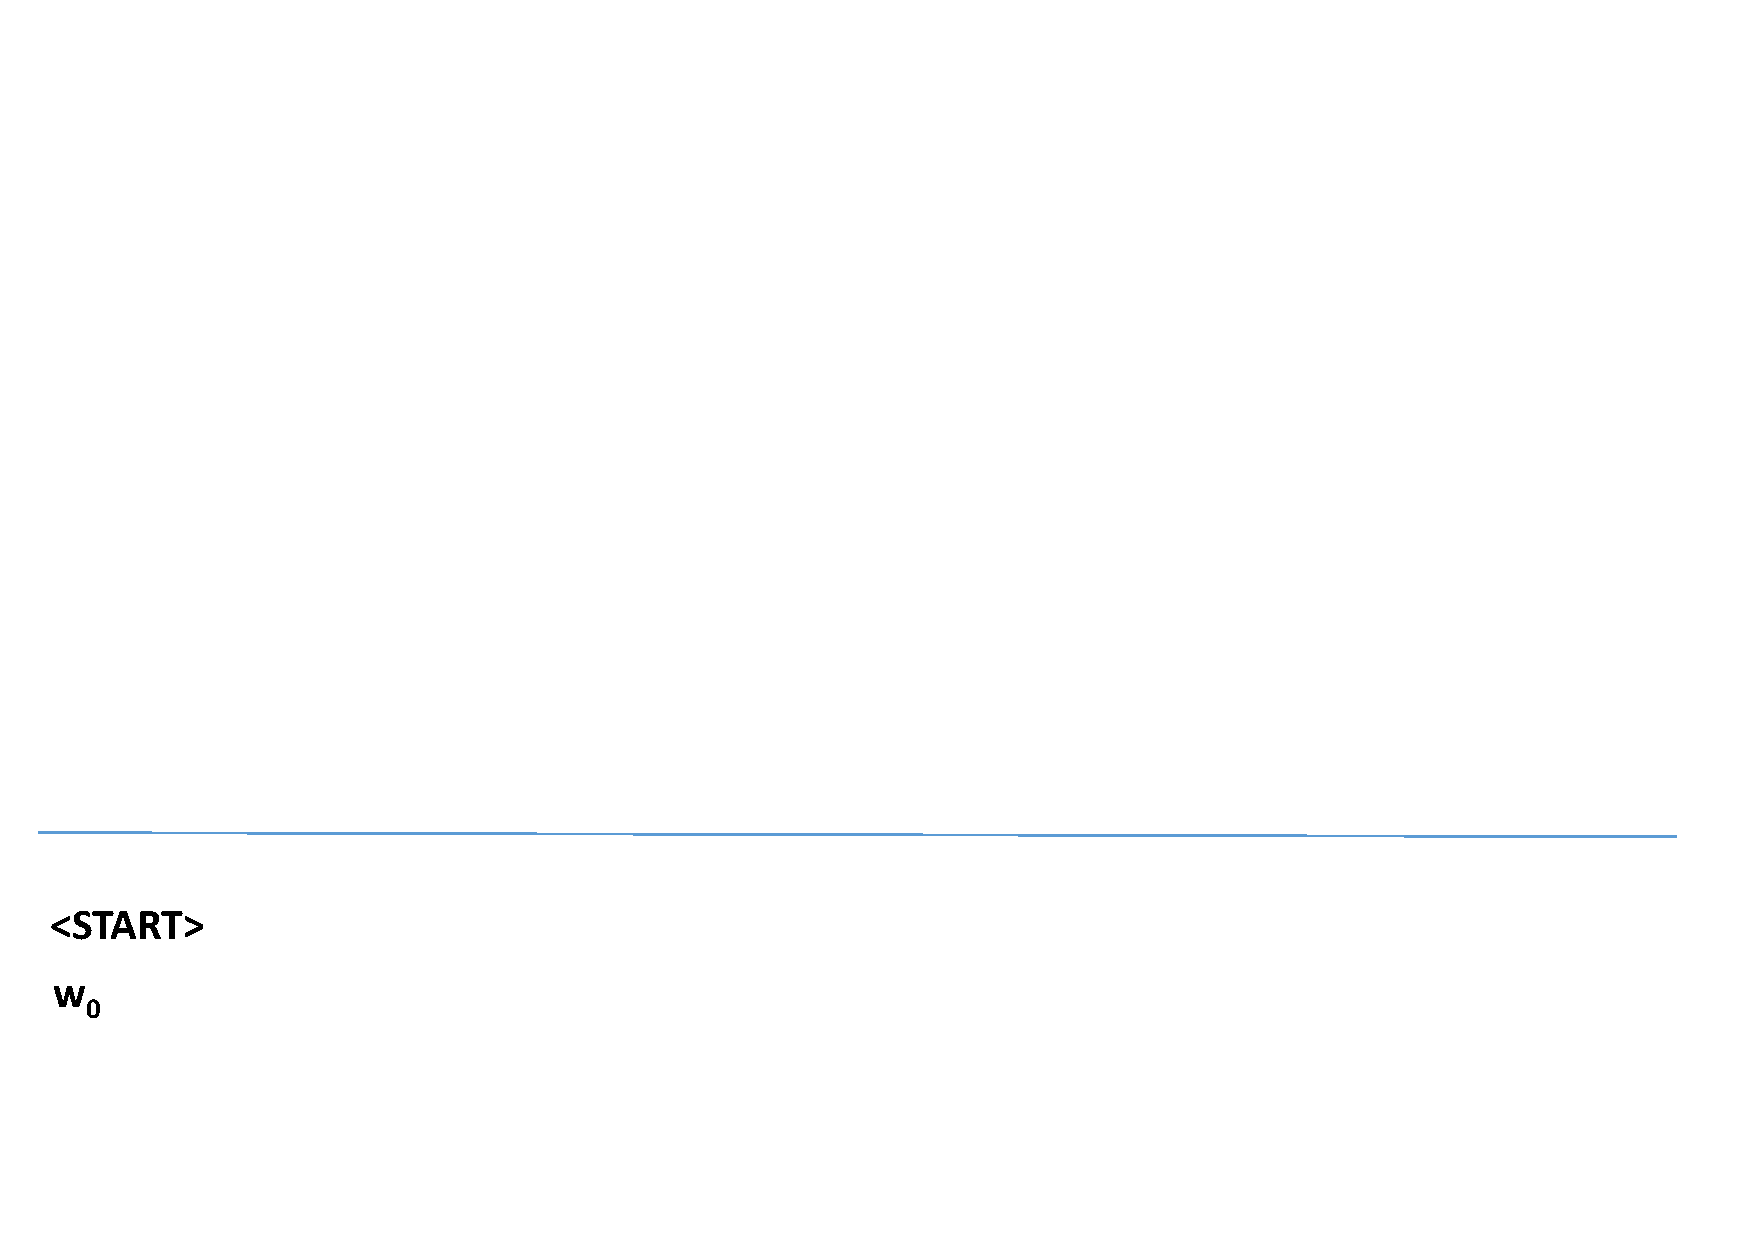
\includegraphics[width=8.67cm,page=1]{figure/arlm.pdf}
	\end{figure}
	\vfill
\end{frame}

% ------------------------------------------------------------------------------

\begin{frame}[noframenumbering]{arlm: toy example}
	\vfill
	\begin{figure}
		\centering
		\includegraphics[width=8.67cm,page=2]{figure/arlm.pdf}
	\end{figure}
	\vfill
\end{frame}
\begin{frame}[noframenumbering]{arlm: toy example}
	\vfill
	\begin{figure}
		\centering
		\includegraphics[width=8.67cm,page=3]{figure/arlm.pdf}
	\end{figure}
	\vfill
\end{frame}
\begin{frame}[noframenumbering]{arlm: toy example}
	\vfill
	\begin{figure}
		\centering
		\includegraphics[width=8.67cm,page=4]{figure/arlm.pdf}
	\end{figure}
	\vfill
\end{frame}
\begin{frame}[noframenumbering]{arlm: toy example}
	\vfill
	\begin{figure}
		\centering
		\includegraphics[width=8.67cm,page=5]{figure/arlm.pdf}
	\end{figure}
	\vfill
\end{frame}
\begin{frame}[noframenumbering]{arlm: toy example}
	\vfill
	\begin{figure}
		\centering
		\includegraphics[width=8.67cm,page=6]{figure/arlm.pdf}
	\end{figure}
	\vfill
\end{frame}
\begin{frame}[noframenumbering]{arlm: toy example}
	\vfill
	\begin{figure}
		\centering
		\includegraphics[width=8.67cm,page=7]{figure/arlm.pdf}
	\end{figure}
	\vfill
\end{frame}
\begin{frame}[noframenumbering]{arlm: toy example}
	\vfill
	\begin{figure}
		\centering
		\includegraphics[width=8.67cm,page=8]{figure/arlm.pdf}
	\end{figure}
	\vfill
\end{frame}
\begin{frame}[noframenumbering]{arlm: toy example}
	\vfill
	\begin{figure}
		\centering
		\includegraphics[width=8.67cm,page=9]{figure/arlm.pdf}
	\end{figure}
	\vfill
\end{frame}
\begin{frame}[noframenumbering]{arlm: toy example}
	\vfill
	\begin{figure}
		\centering
		\includegraphics[width=8.67cm,page=10]{figure/arlm.pdf}
	\end{figure}
	\vfill
\end{frame}
\begin{frame}[noframenumbering]{arlm: toy example}
	\vfill
	\begin{figure}
		\centering
		\includegraphics[width=8.67cm,page=11]{figure/arlm.pdf}
	\end{figure}
	\vfill
\end{frame}
\begin{frame}[noframenumbering]{arlm: toy example}
	\vfill
	\begin{figure}
		\centering
		\includegraphics[width=8.67cm,page=12]{figure/arlm.pdf}
	\end{figure}
	\vfill
\end{frame}
\begin{frame}[noframenumbering]{arlm: toy example}
	\vfill
	
	\begin{figure}
		\centering
		\includegraphics[width=8.67cm,page=13]{figure/arlm.pdf}
	\end{figure}
	
	\vfill
\end{frame}

% ------------------------------------------------------------------------------

\begin{frame}{arlm: probabilistic interpretation}

\vfill

\begin{itemize}
	\item Gives an estimate for the probability of a sentence using conditional probabilities
	\item In general: $$ P(A \cap B) = P(B) \cdot P(A | B)$$
	\item For $P(sentence)$:
	$$ P(w_1, w_2, \dots, w_n | w_0)$$ $$ = P(w_1 | w_0) \cdot P(w_2 | w_0, w_1) \cdot \hdots \cdot P(w_n | w_0, \dots, w_{n-1})$$
\end{itemize}

\vfill

\end{frame}

% ------------------------------------------------------------------------------

\begin{frame}{Examples of ARLMs (1)}

\vfill

\textbf{Neural Machine Translation:}

	\begin{figure}
		\centering
		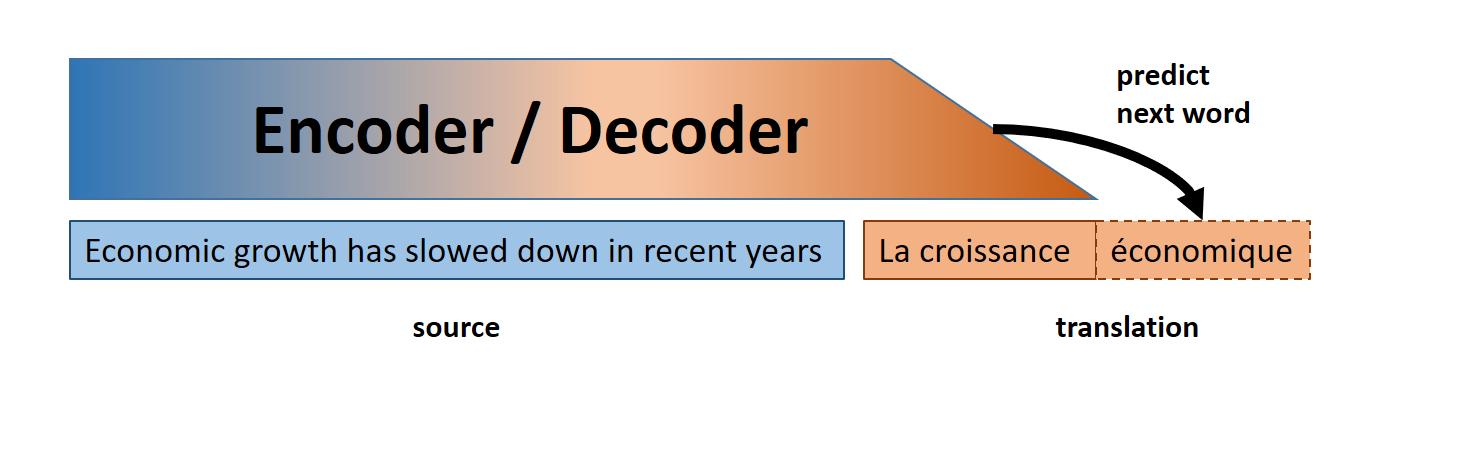
\includegraphics[width=12cm]{figure/arlm1.png}
	\end{figure}
	
\vfill

\end{frame}

% ------------------------------------------------------------------------------

\begin{frame}{Examples of ARLMs (1)}

\vfill

\textbf{Image Captioning:}

	\begin{figure}
		\centering
		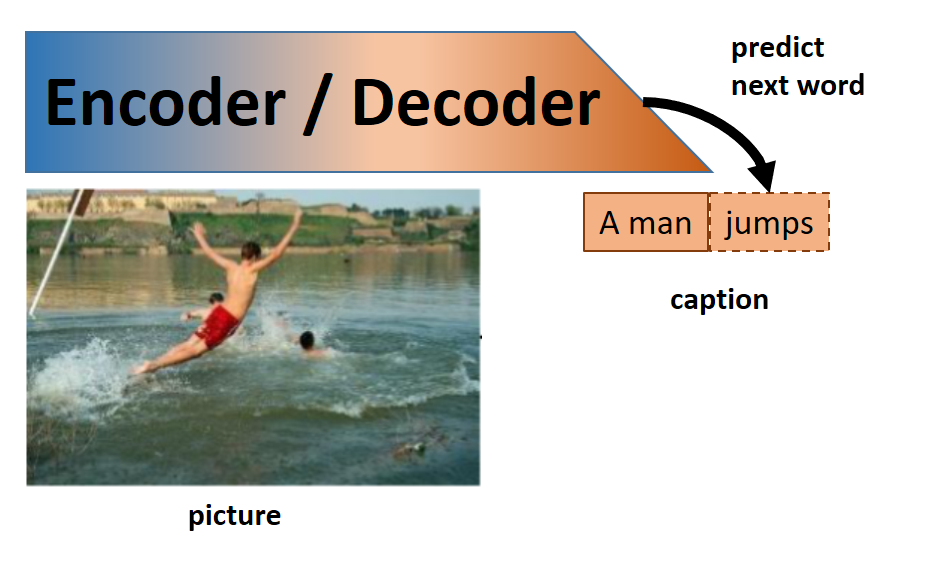
\includegraphics[width=8cm]{figure/arlm2.png}
	\end{figure}
\vfill

\end{frame}

%%%%%%%%%%%%%%%%%%%%%%%%%%%%%%%%%%%%%%%%%%%%%%%%%%%%%%%%%%%%%%%%%%%%
\section{GPT-1}
%%%%%%%%%%%%%%%%%%%%%%%%%%%%%%%%%%%%%%%%%%%%%%%%%%%%%%%%%%%%%%%%%%%%
% Source: DL4NLP chapter07-gpt/slides-71-gpt.tex

\begin{frame}{GPT-1}

\vfill

	\begin{figure}
		\centering
		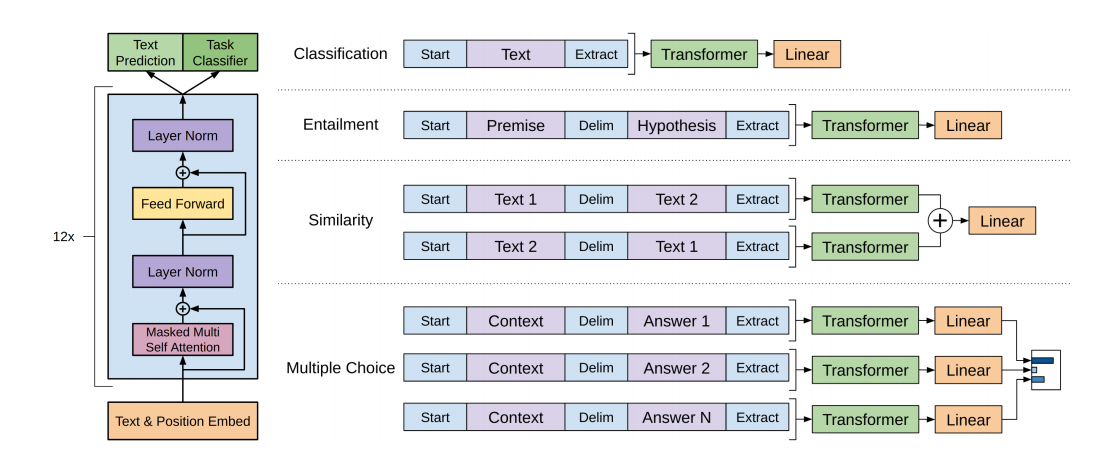
\includegraphics[width = 12cm]{figure/71-gpt}\\
		\citebutton{Source: Radford et al., 2018}{https://openai.com/blog/language-unsupervised/}
	\end{figure}

\vfill

\end{frame}

% ------------------------------------------------------------------------------

\begin{frame}{Architectural details}

\vfill

	\begin{itemize}
		\item Transformer \textit{decoder} as backbone of the architecture
			\begin{itemize}
				\item 12-layer-decoder with masked self-attention mechanism
				\item Hidden dimension $H = 768$, $A = 12$ Attention heads
				\item BPE vocabulary w/ 40k merges
				\item Learned positional embeddings (as opposed to fixed, sinusoidal ones in the original Transformer)
			\end{itemize}
		\item With $U = (w_{t-k}, \hdots, w_{t-1})$
\begin{align*}
	\vec h_0 &= \vec U \vec W_e + \vec W_p \\
	\vec h_l &= Trafo(\vec h_{l-1}) \forall l \in [1,n]\\
	P(w_t) &= softmax(\vec h_n \vec W_e^\top)
\end{align*}
	\end{itemize}

\vfill

\end{frame}

% ------------------------------------------------------------------------------

\begin{frame}{Pre-Training GPT}

\vfill

\begin{itemize}
		\item Standard LM objective

\begin{align*}
	L_1(\{w_1, \hdots, w_n\}) = \sum_i \log(P(w_t | w_{t-k}, \hdots, w_{t-1}; \Theta))
\end{align*}
					
					where $\{w_1, \hdots, w_n\}$ is an \textit{unlabeled} sequence of tokens

		\item \textit{Resource:} BooksCorpus 
			\begin{itemize}
				\item > 7k unpublished books from various genres
				\item contains long texts and thus allows learning long range dependencies
			\end{itemize}
\end{itemize}

\vfill

\end{frame}

% ------------------------------------------------------------------------------

\begin{frame}{Fine-Tuning GPT}

\vfill
			
\begin{itemize}
		\item Linear output layer with softmax activation on top
		\item Auxiliary language modeling objective during fine-tuning\\
					$\rightarrow$ Improves generalization\\
					$\rightarrow$ Accelerates convergence
		\item Task-specific input transformations
					\begin{itemize}
						\item \textit{Entailment:} \\ Concatenation of premise ($p$) \& hypothesis ($h$): $[p; \$; h]$
						\item \textit{Similarity:} Use both orderings and concatenate resulting representations: $[s_1; \$; s_2]$ and $[s_2; \$; s_1]$
						\item \textit{Q\&A and Commensense Reasoning:} \\ Concatenate context ($z$), question ($q$) and each possible answer ($a_k$): $[z; q; \$, a_k]$
					\end{itemize}
		\item Fine-tuning is rather quick, 3 epochs were sufficient
\end{itemize}

\vfill

\end{frame}

% ------------------------------------------------------------------------------

\begin{frame}{Fine-Tuning GPT}

\vfill

\begin{itemize}
		\item Additional objective:
					\begin{align*}
						L_2(\{w_1, \hdots, w_n\}) = \sum_{x,y} \log(P(y | w_1, \hdots, w_n))
					\end{align*}		
					where 
				\begin{itemize}
					\item $P(y | w_1, \hdots, w_n) = softmax(h_l^m W_y)$ and 
					\item $\{w_1, \hdots, w_n\}$ is a \textit{labeled} sequence of tokens
				\end{itemize}
		\item Combining both objectives: 
					\begin{align*}
						L_3(\{w_1, \hdots, w_n\}) = L_2(\{w_1, \hdots, w_n\}) + \lambda \cdot L_1(\{w_1, \hdots, w_n\})
					\end{align*}
\end{itemize}

\vfill

\end{frame}

% ------------------------------------------------------------------------------

\begin{frame}{SOTA results}

\vfill

	\textbf{Performance on different benchmarks:}

	\begin{figure}
		\centering
		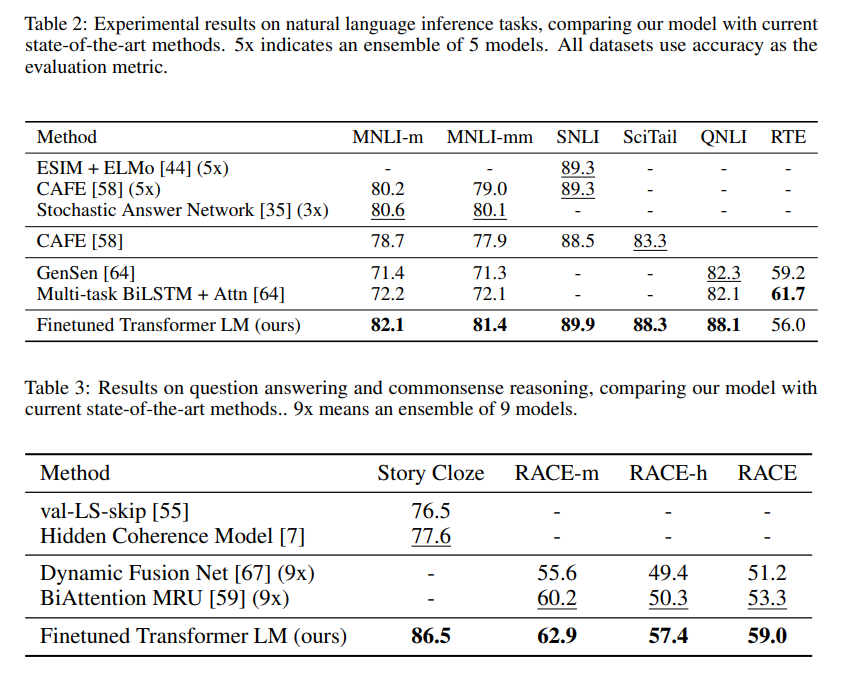
\includegraphics[width = 6.80cm]{figure/gpt-sota.png}\\ 
		\citebutton{Source: Radford et al., 2018}{https://openai.com/blog/language-unsupervised/}
	\end{figure}

\vfill

\end{frame}

% ------------------------------------------------------------------------------

%%%%%%%%%%%%%%%%%%%%%%%%%%%%%%%%%%%%%%%%%%%%%%%%%%%%%%%%%%%%%%%%%%%%
\section{GPT-2}
%%%%%%%%%%%%%%%%%%%%%%%%%%%%%%%%%%%%%%%%%%%%%%%%%%%%%%%%%%%%%%%%%%%%
% Source: DL4NLP chapter07-gpt/slides-72-gpt2.tex

\begin{frame}{Starting with a controversy}

\vfill

\begin{figure}
\centering
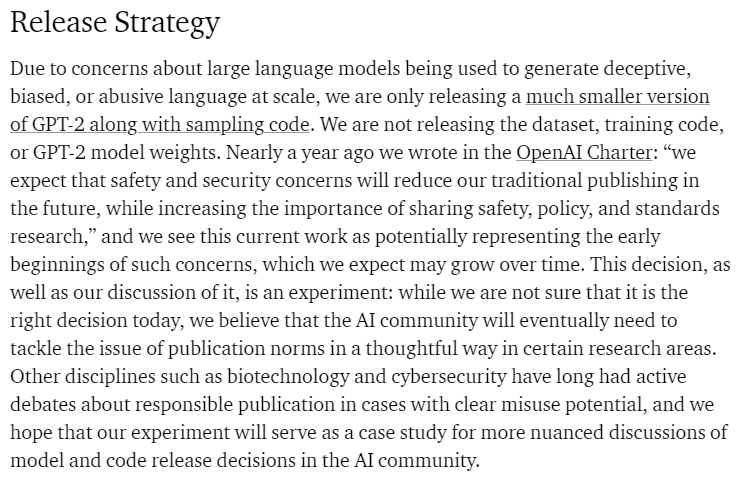
\includegraphics[width = 9cm]{figure/72-gpt2-release.png}\\ 
\citebutton{Source: OpenAI Blog}{https://openai.com/research/better-language-models}
\end{figure}

\vfill

\end{frame}

% ------------------------------------------------------------------------------

\begin{frame}{The architecture}

\vfill

\begin{itemize}
	\item Transformer decoder pre-trained on AR language modeling
	\item Custom web scrape (not publicly available) of all outbound links from Reddit
	\item[$\to$] 8M documents / 40GB of text
	\item Byte-level BPE for tokenization
	\item Increased context size: $512 \to 1024$
\end{itemize}

\begin{figure}
\centering
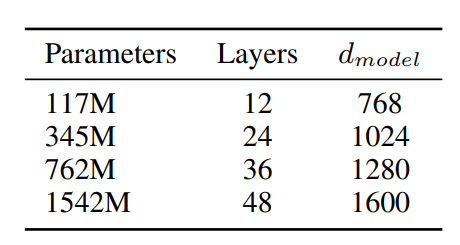
\includegraphics[width = 6cm]{figure/72-gpt2-size.png}\\ 
\citebutton{Source: Radford et al., 2019}{https://openai.com/research/better-language-models}
\end{figure}

\vfill

\end{frame}

% ------------------------------------------------------------------------------

\begin{frame}{Language models as multitask learners}

\vfill

\begin{itemize}

\item[] ``But as exemplified in McCann et al. (2018), language
	provides a flexible way to specify tasks, inputs,
	and outputs all as a sequence of symbols.

\item[] For
	example, a translation training
	example can be written as the sequence (translate to
	french, english text, french text).''
	\item Model benefits from seeing ``natural`` occurrences of task demonstrations during pre-training on large-scale web corpora
	\item[] $\to$ Related rationale to T5 (\textit{literal task descriptions}), but slightly different (\textit{acquired on the fly already during pre-training}).
\end{itemize}

\begin{figure}
\centering
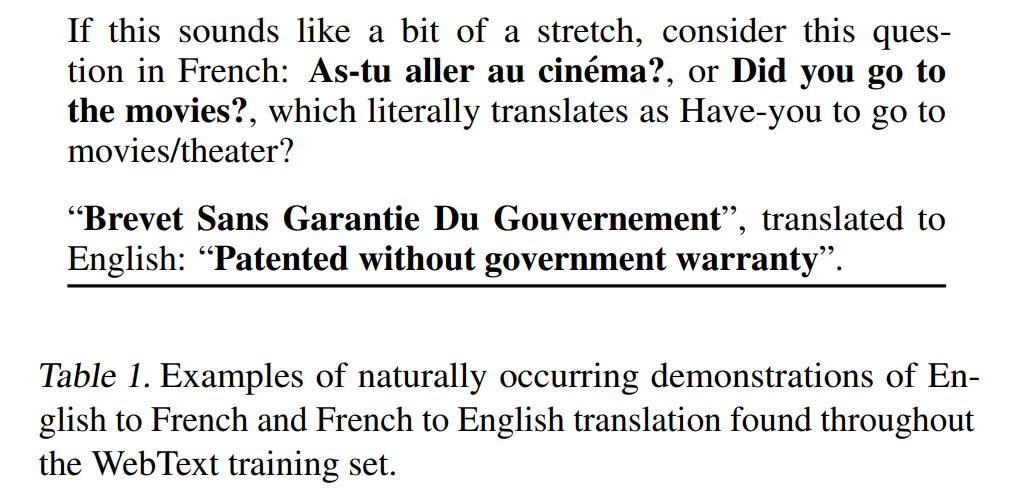
\includegraphics[width = 2.63cm]{figure/72-gpt2-demo-wild.png}\\ 
\citebutton{Source: Radford et al., 2019}{https://openai.com/research/better-language-models}
\end{figure}

\vfill

\end{frame}

% ------------------------------------------------------------------------------

\begin{frame}{Capabilities -- Zero-Shot}

\vfill

\pause
\begin{itemize}
	\item \textit{Zero-shot} refers to solving a task which the model was not previously explicitly trained on, just providing it with a description of the task but no demonstrations, i.e. input/output pairs.
	\item \textit{Few-shot} would be a relaxation of this setting, allowing for also providing the models with demonstrations (but still no training/gradient updates).
	\item Radford et al. show GPT-2's zero-shot capabilities on a range of different tasks, paving the way for the developments that came with GPT-3.
\end{itemize}

\vfill

\end{frame}

% ------------------------------------------------------------------------------

\begin{frame}{Capabilities -- Zero-Shot}

\vfill

\begin{figure}
\centering
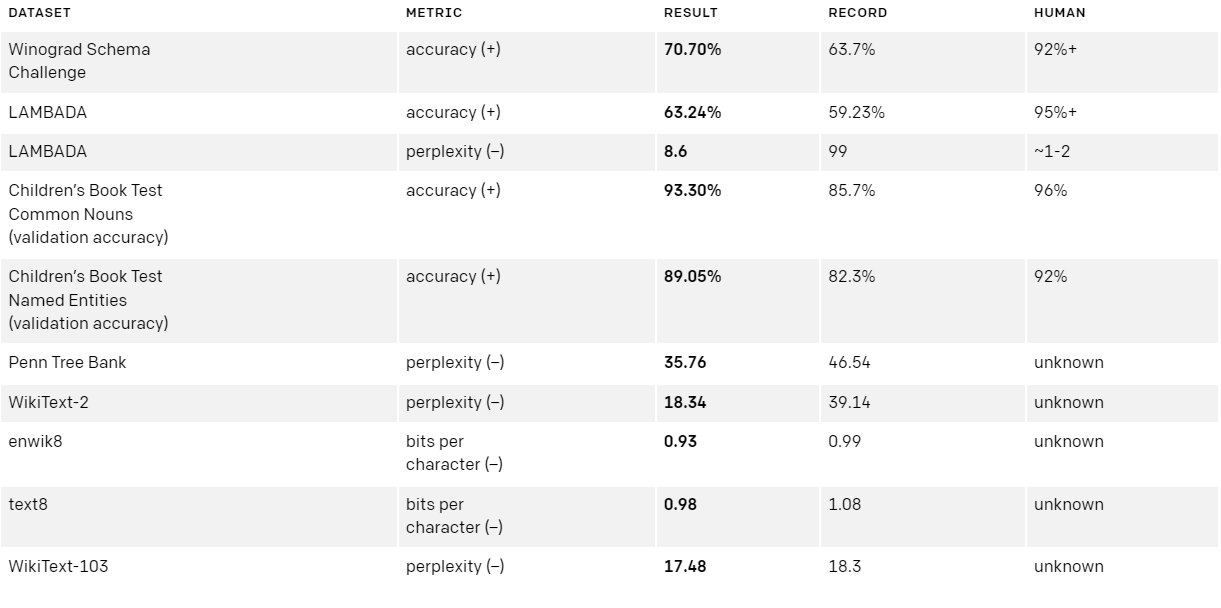
\includegraphics[width = 11cm]{figure/72-gpt2-zeroshot.png}\\ 
\citebutton{Source: Radford et al., 2019}{https://openai.com/research/better-language-models}
\end{figure}

\vfill

\footnotesize{(Note: The numbers correspond to the last row of the Table on the slide ``The architecture'')}

\end{frame}

%%%%%%%%%%%%%%%%%%%%%%%%%%%%%%%%%%%%%%%%%%%%%%%%%%%%%%%%%%%%%%%%%%%%
\section{GPT-3 and In-Context Learning}
%%%%%%%%%%%%%%%%%%%%%%%%%%%%%%%%%%%%%%%%%%%%%%%%%%%%%%%%%%%%%%%%%%%%
% Source: DL4NLP chapter07-gpt/slides-73-gpt3xshot.tex

\begin{frame}{Prompting}

\vfill

  \begin{itemize}
\item Salesforce/GPT2: solve tasks by generation through
minor reformatting of original tasks (e.g., generate answer
in QA, generate label in classification)
\item Prompting: solve tasks by generation through carefully
designed prompts/instructions that are very different
from the original talk description.
\item Prompting is usually used within in-context learning
(zero-shot, one-shot, few-shot)
\item prompting = instruction = task description = pattern
    \end{itemize}

\vfill

\end{frame}

% ------------------------------------------------------------------------------

\begin{frame}{in-context learning}

\vfill

\begin{figure}
		\centering
		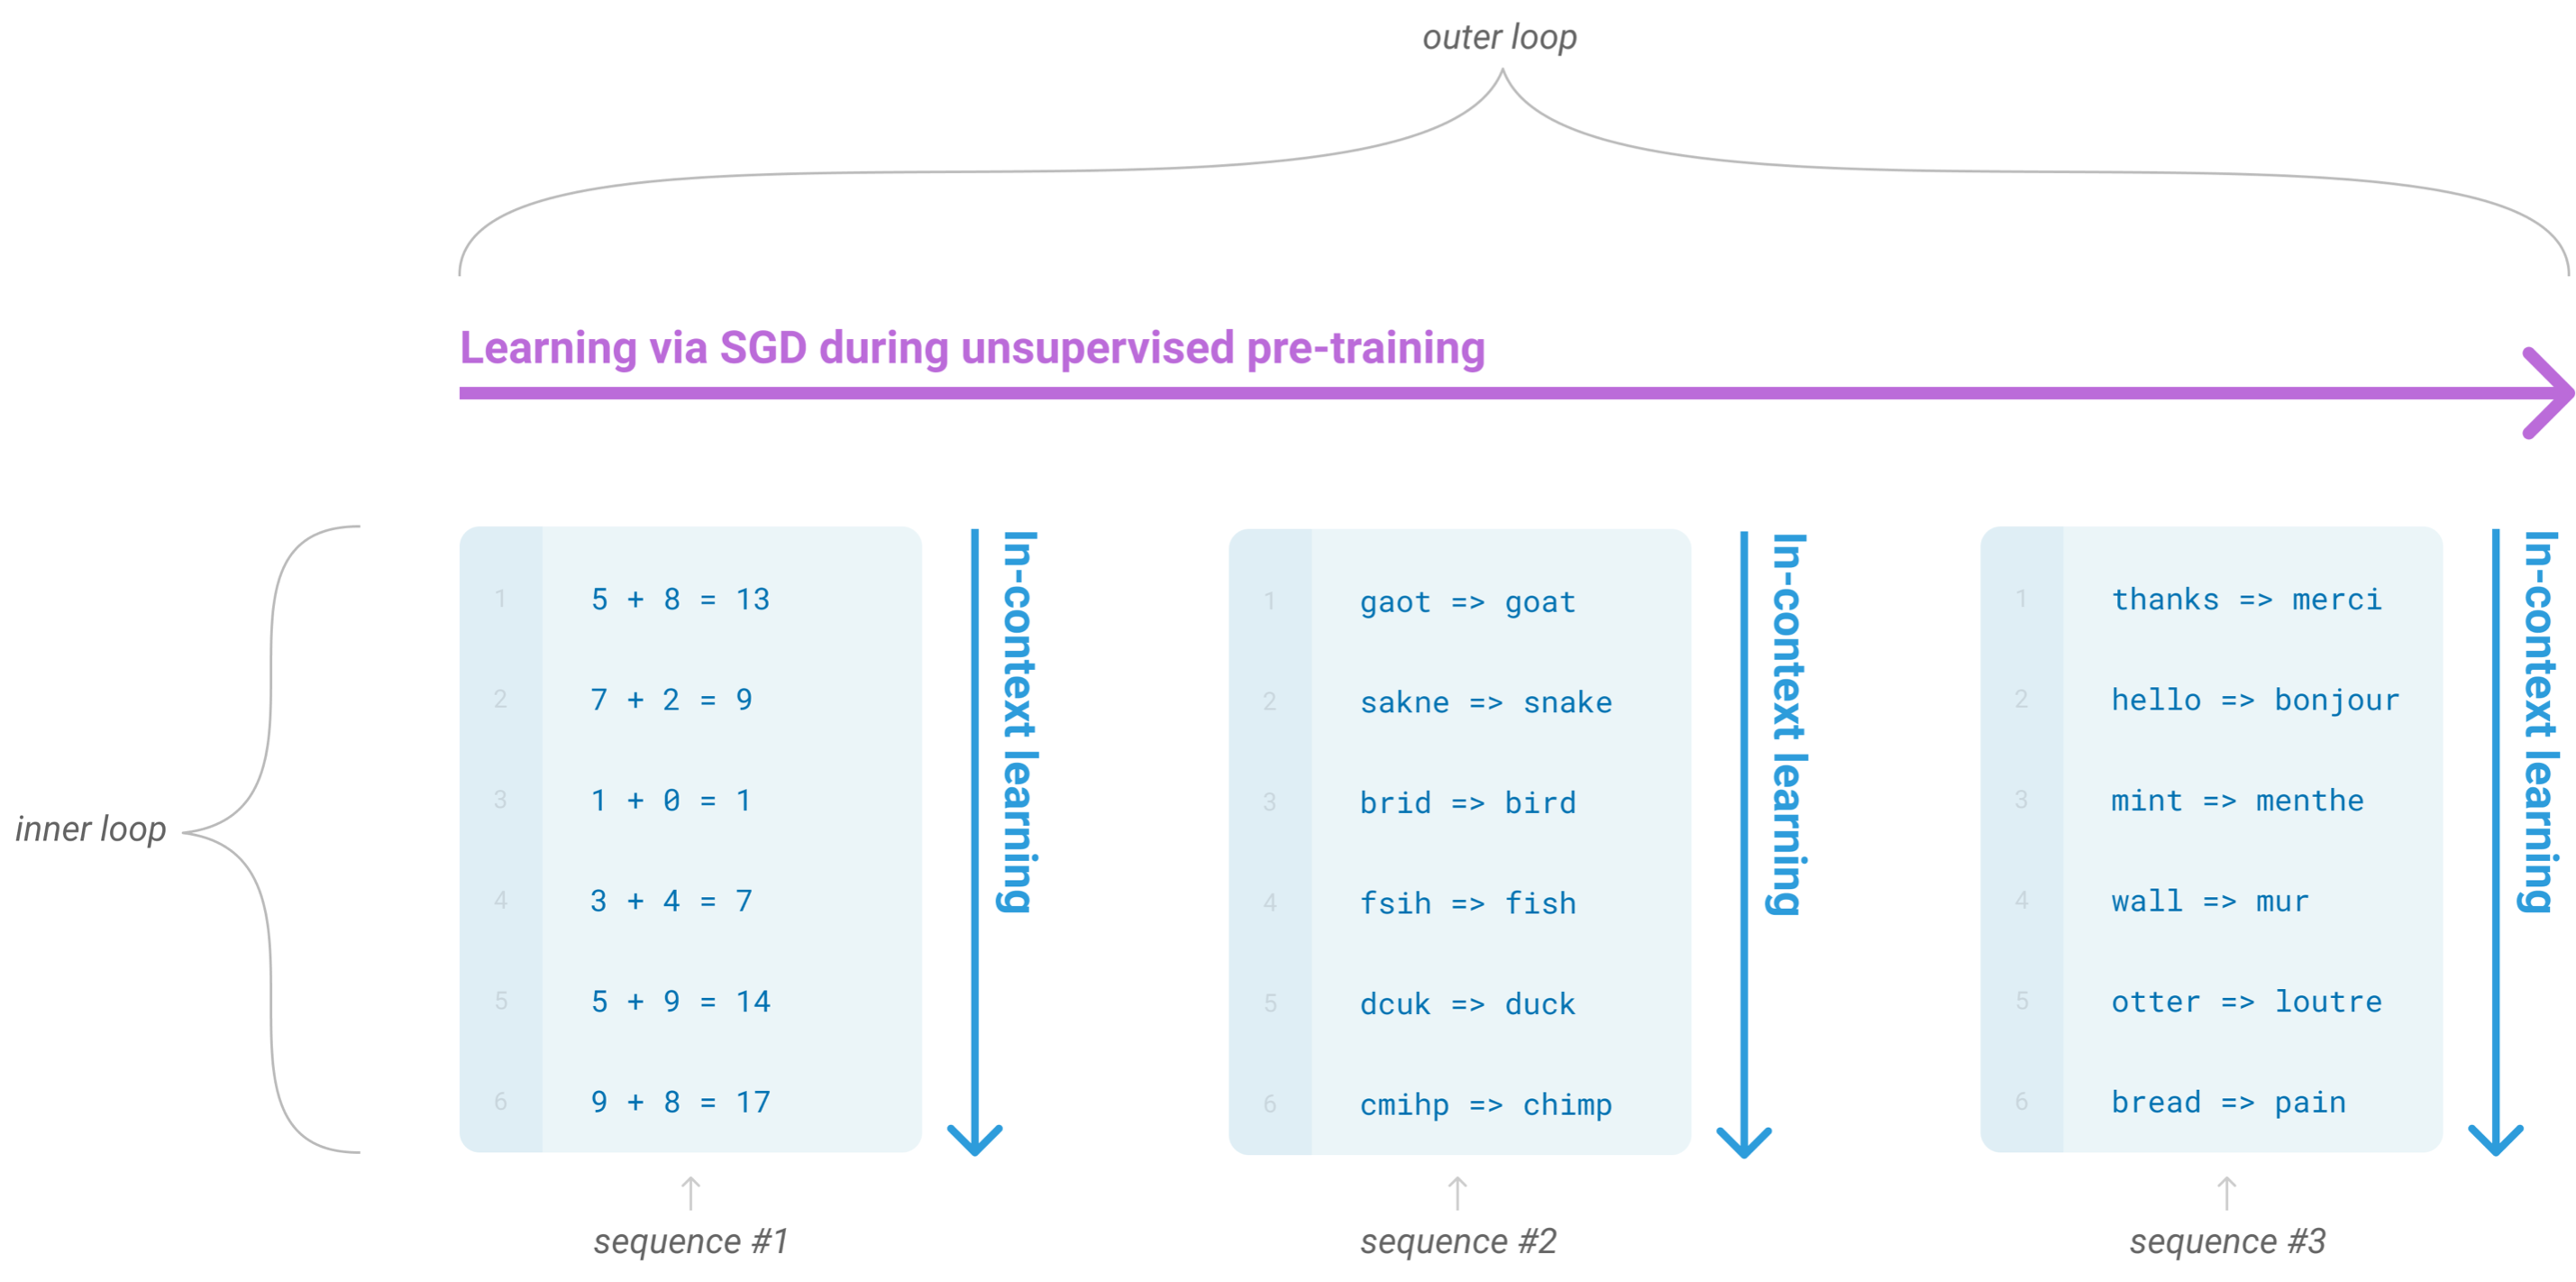
\includegraphics[clip,trim=200px 0 0 0,width=\linewidth]{figure/twotypesoflearning.png}\\
		\citebutton{Source: Brown et al., 2020}{https://arxiv.org/abs/2005.14165}
	\end{figure}

\vfill

\end{frame}

% ------------------------------------------------------------------------------

\begin{frame}{in-context learning}

\vfill

\begin{figure}
		\centering
		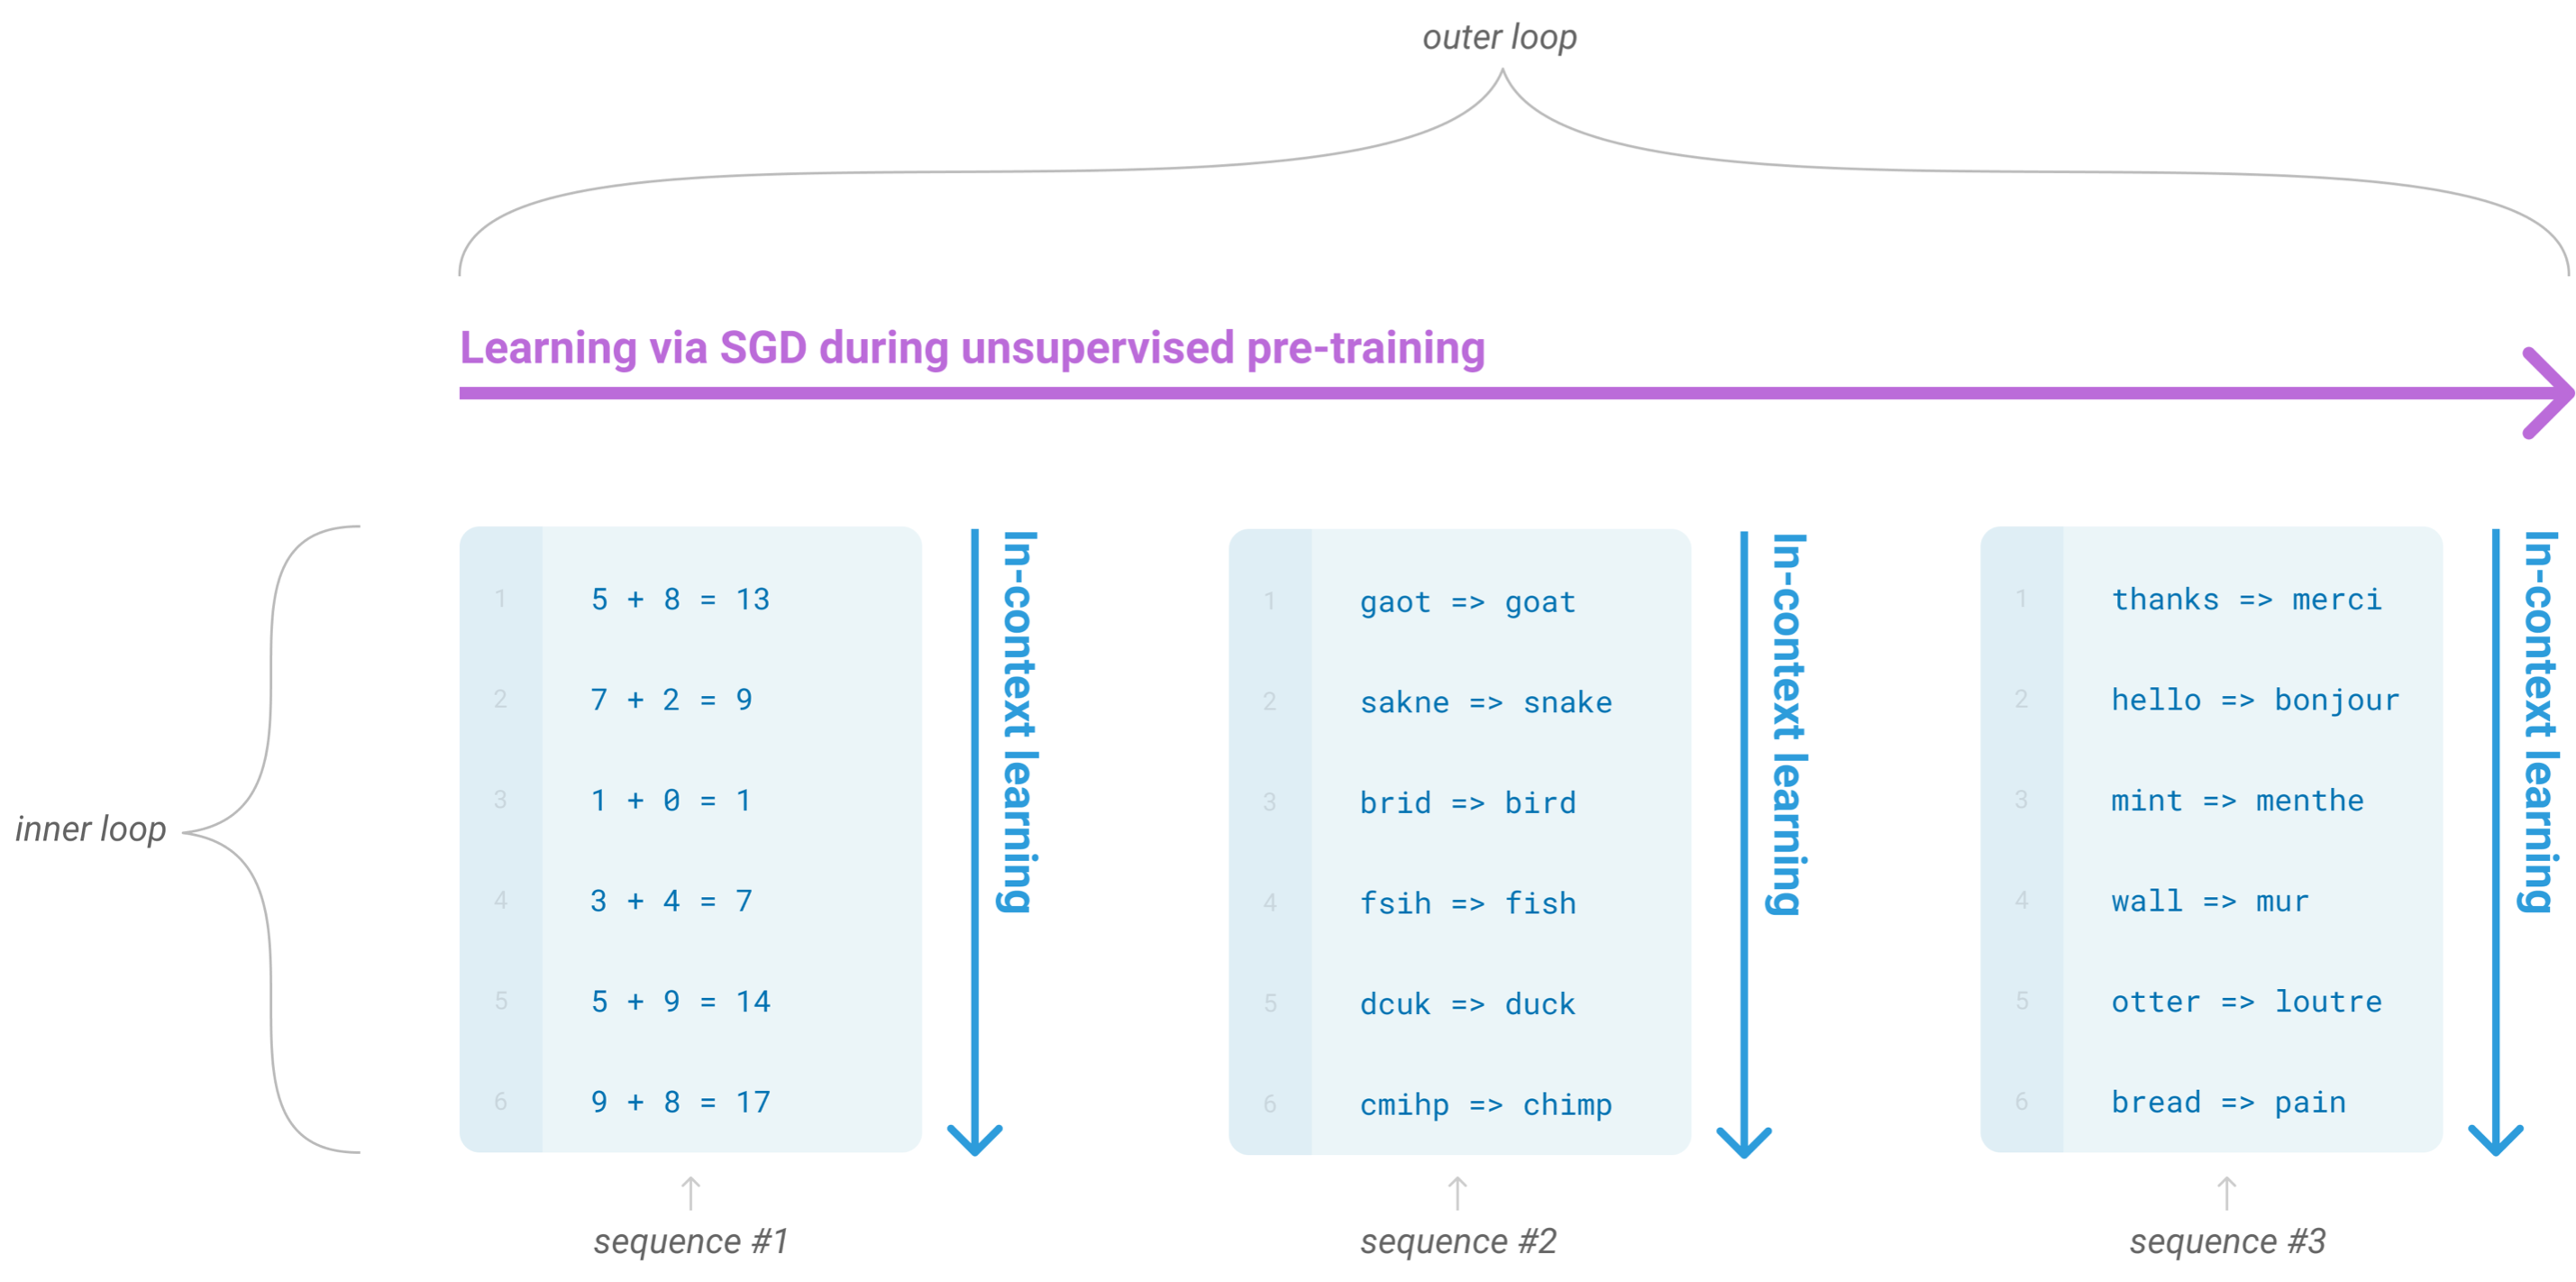
\includegraphics[width = 6cm]{figure/twotypesoflearning.png}\\
		\citebutton{Source: Brown et al., 2020}{https://arxiv.org/abs/2005.14165}
\end{figure}

\begin{itemize}
	\item \textbf{Pre-training (Outer loop):}
			\begin{itemize}
				\item Model develops broad set of skills and abilities
				\item Trained via gradient descent
			\end{itemize}
	\item \textbf{Inference (Inner loop):}
			\begin{itemize}
				\item It uses these abilities to rapidly adapt to a desired task\\(\textit{= in-context learning})
				\item Just a single forward pass w/o any gradient updates
			\end{itemize}
\end{itemize}

\vfill

\end{frame}

% ------------------------------------------------------------------------------

\begin{frame}{Zero-shot learning}

\vfill

	\begin{figure}
		\centering
		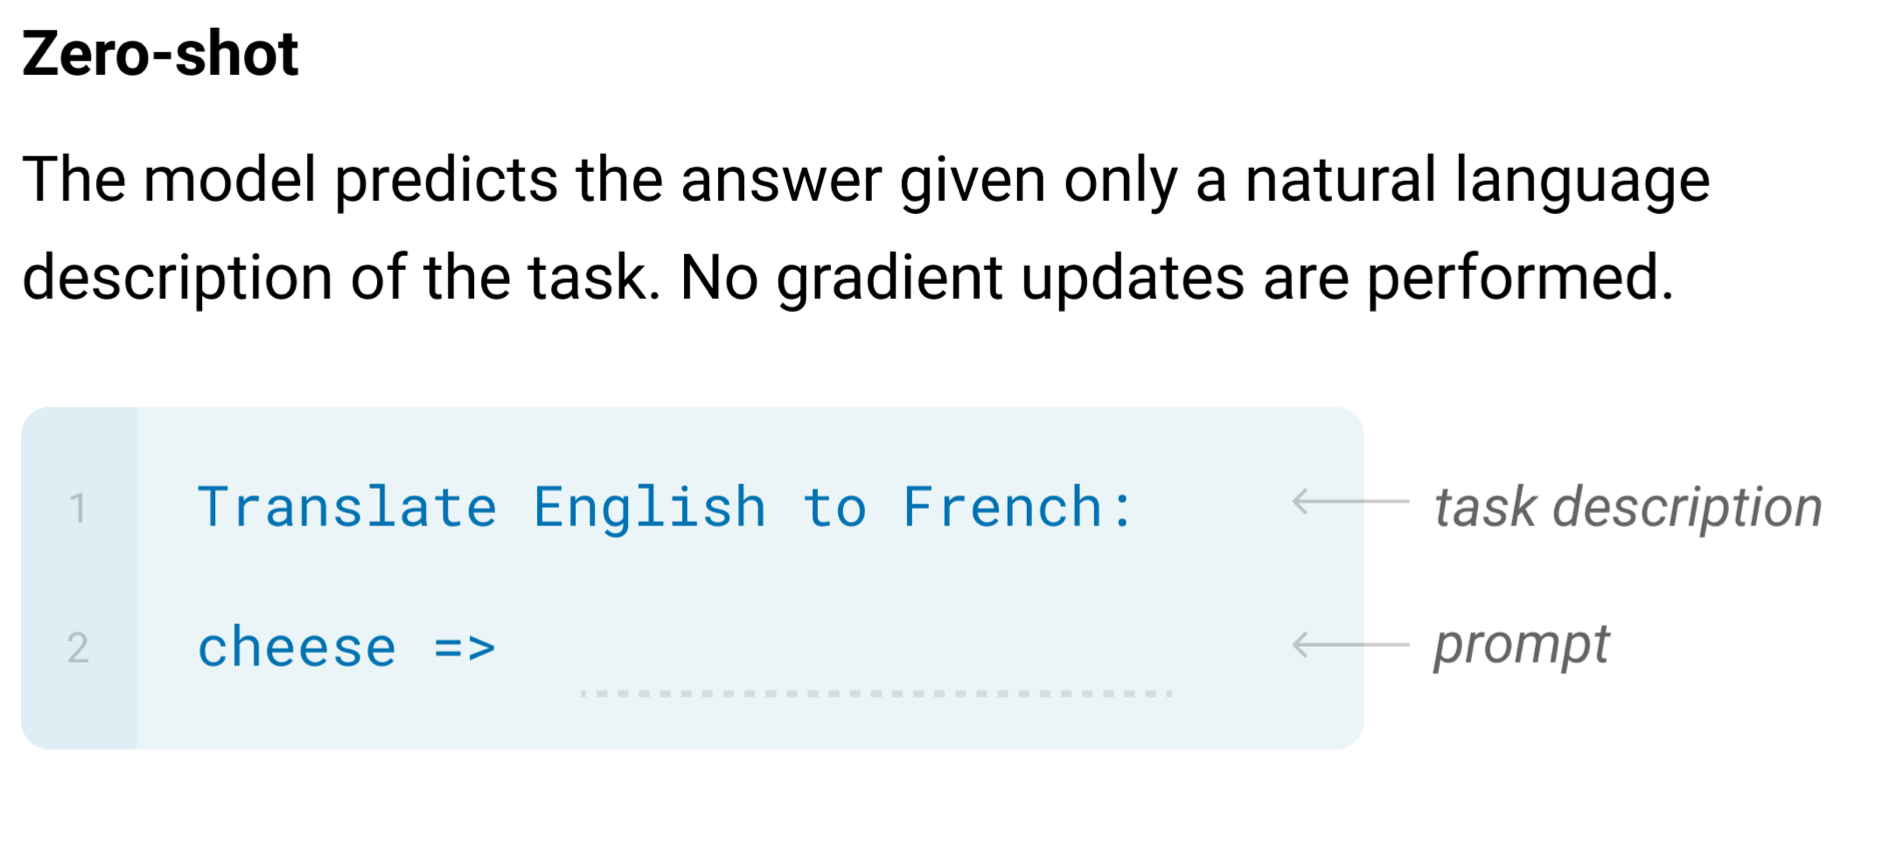
\includegraphics[width=10cm]{figure/gptzeroshot.png}\\
		\citebutton{Source: Brown et al., 2020}{https://arxiv.org/abs/2005.14165}
	\end{figure}

\begin{itemize}
	\item No gradient updates
	\item Learning happens ``on the fly``
	\item Model has to ``understand`` the task description
\end{itemize}

\vfill

\end{frame}

% ------------------------------------------------------------------------------

\begin{frame}{One-shot learning}

\vfill

	\begin{figure}
		\centering
		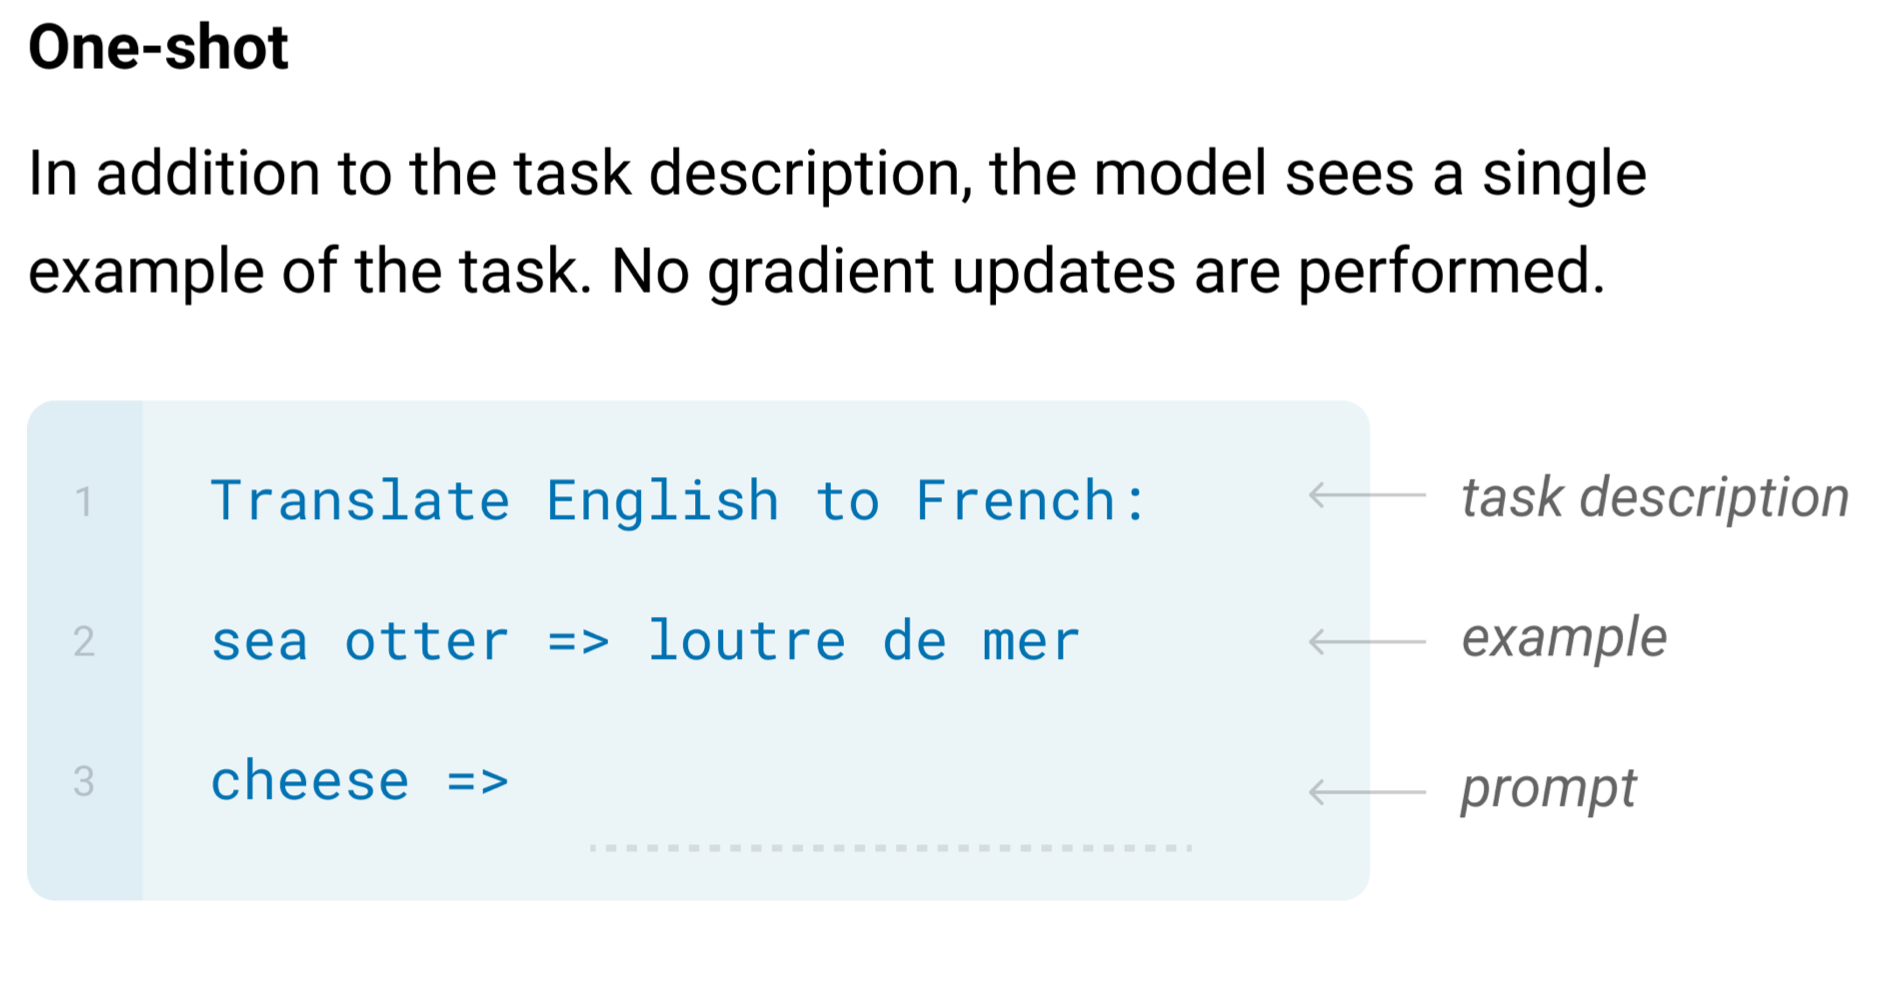
\includegraphics[width=8.50cm]{figure/gptoneshot.png}\\
		\citebutton{Source: Brown et al., 2020}{https://arxiv.org/abs/2005.14165}
	\end{figure}

\begin{itemize}
	\item No gradient updates
	\item Model has to ``understand`` the task description
	\item Understanding supported by \textit{one} demonstration
\end{itemize}

\vfill

\end{frame}

% ------------------------------------------------------------------------------

\begin{frame}{Few-shot learning}

\vfill

	\begin{figure}
		\centering
		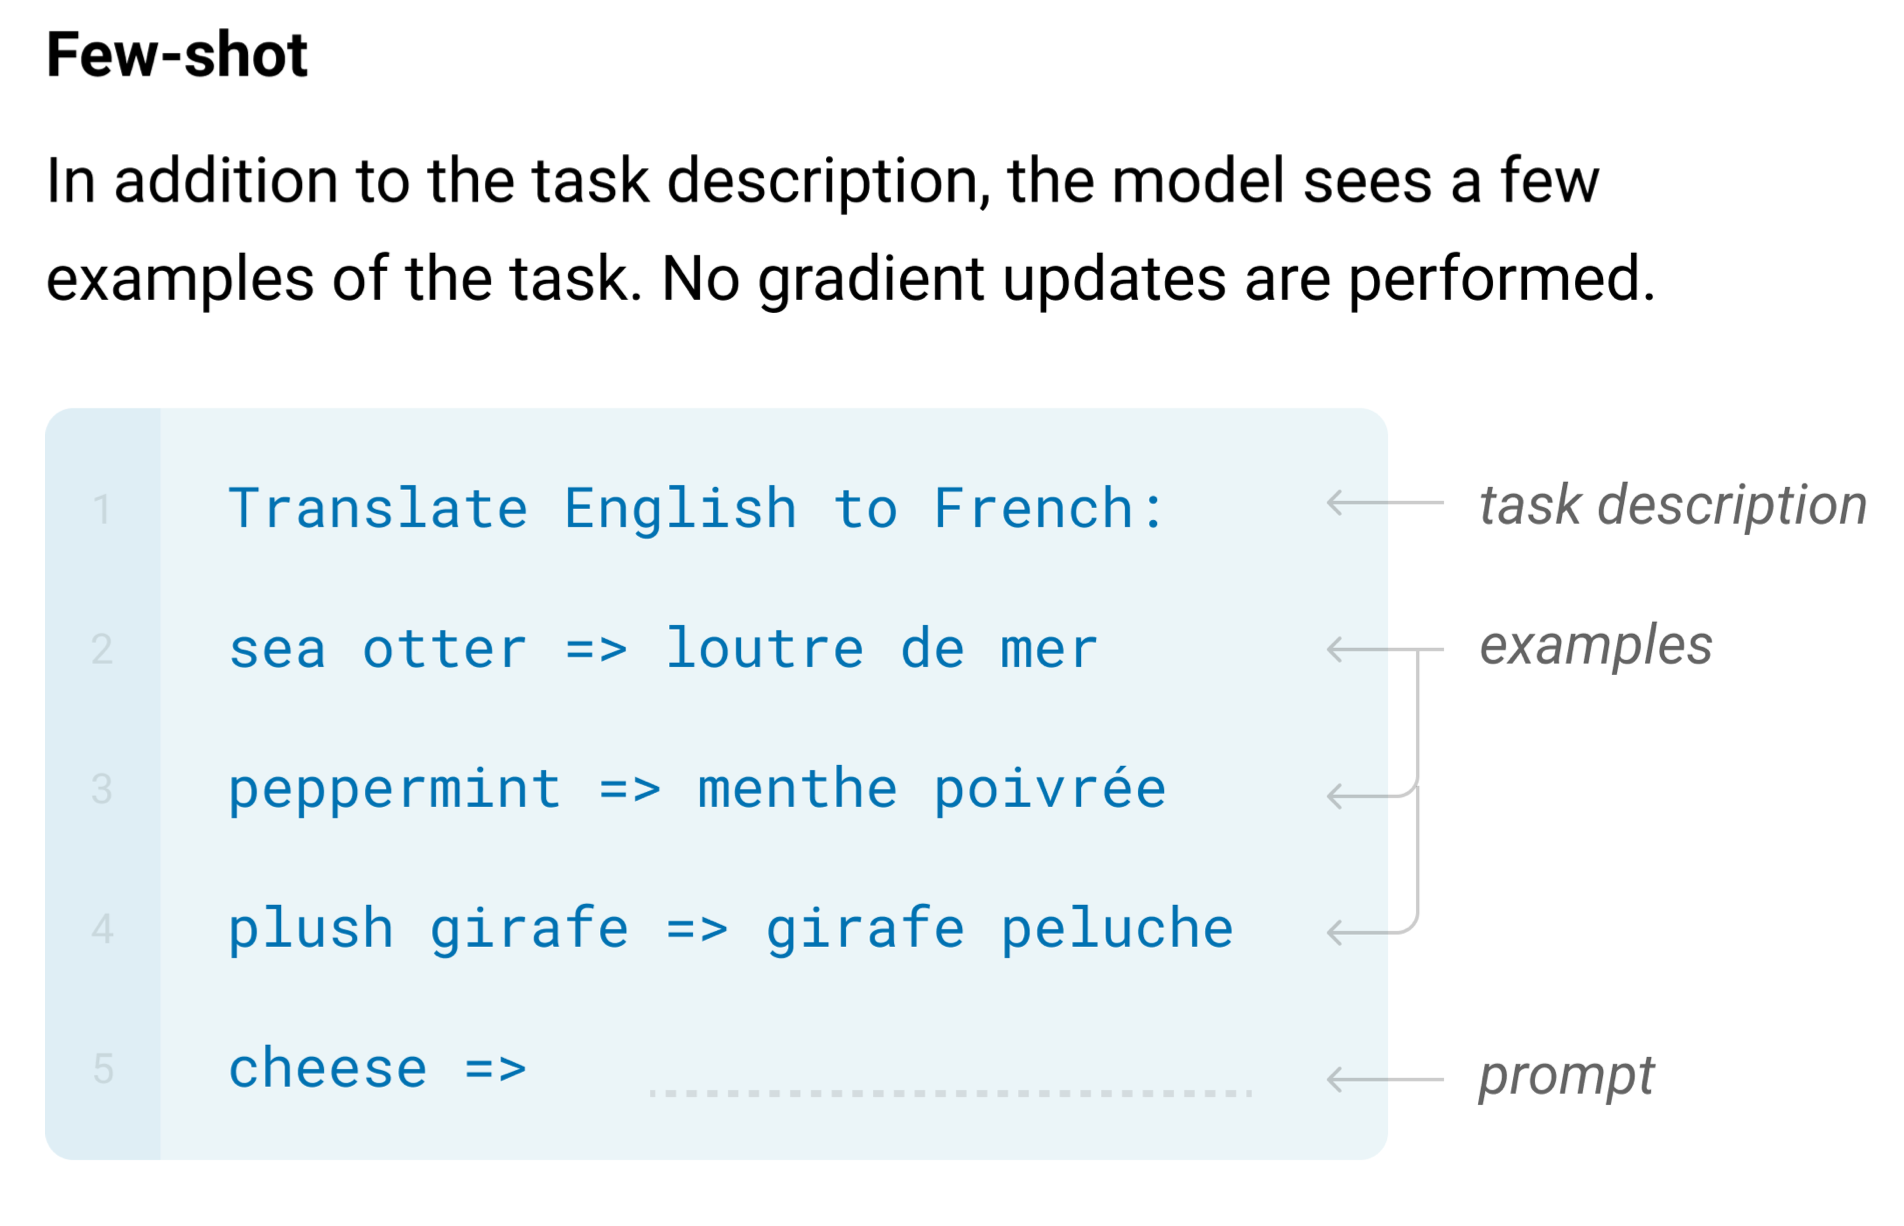
\includegraphics[width=6.80cm]{figure/gptfewshot.png}\\
		\citebutton{Source: Brown et al., 2020}{https://arxiv.org/abs/2005.14165}
	\end{figure}

\begin{itemize}
	\item No gradient updates
	\item Model has to ``understand`` the task description
	\item Understanding supported by \textit{few} demonstrations
\end{itemize}

\vfill

\end{frame}

% ------------------------------------------------------------------------------

\begin{frame}{effective in-context learning*}
	
\vfill
	
\begin{figure}
		\centering
		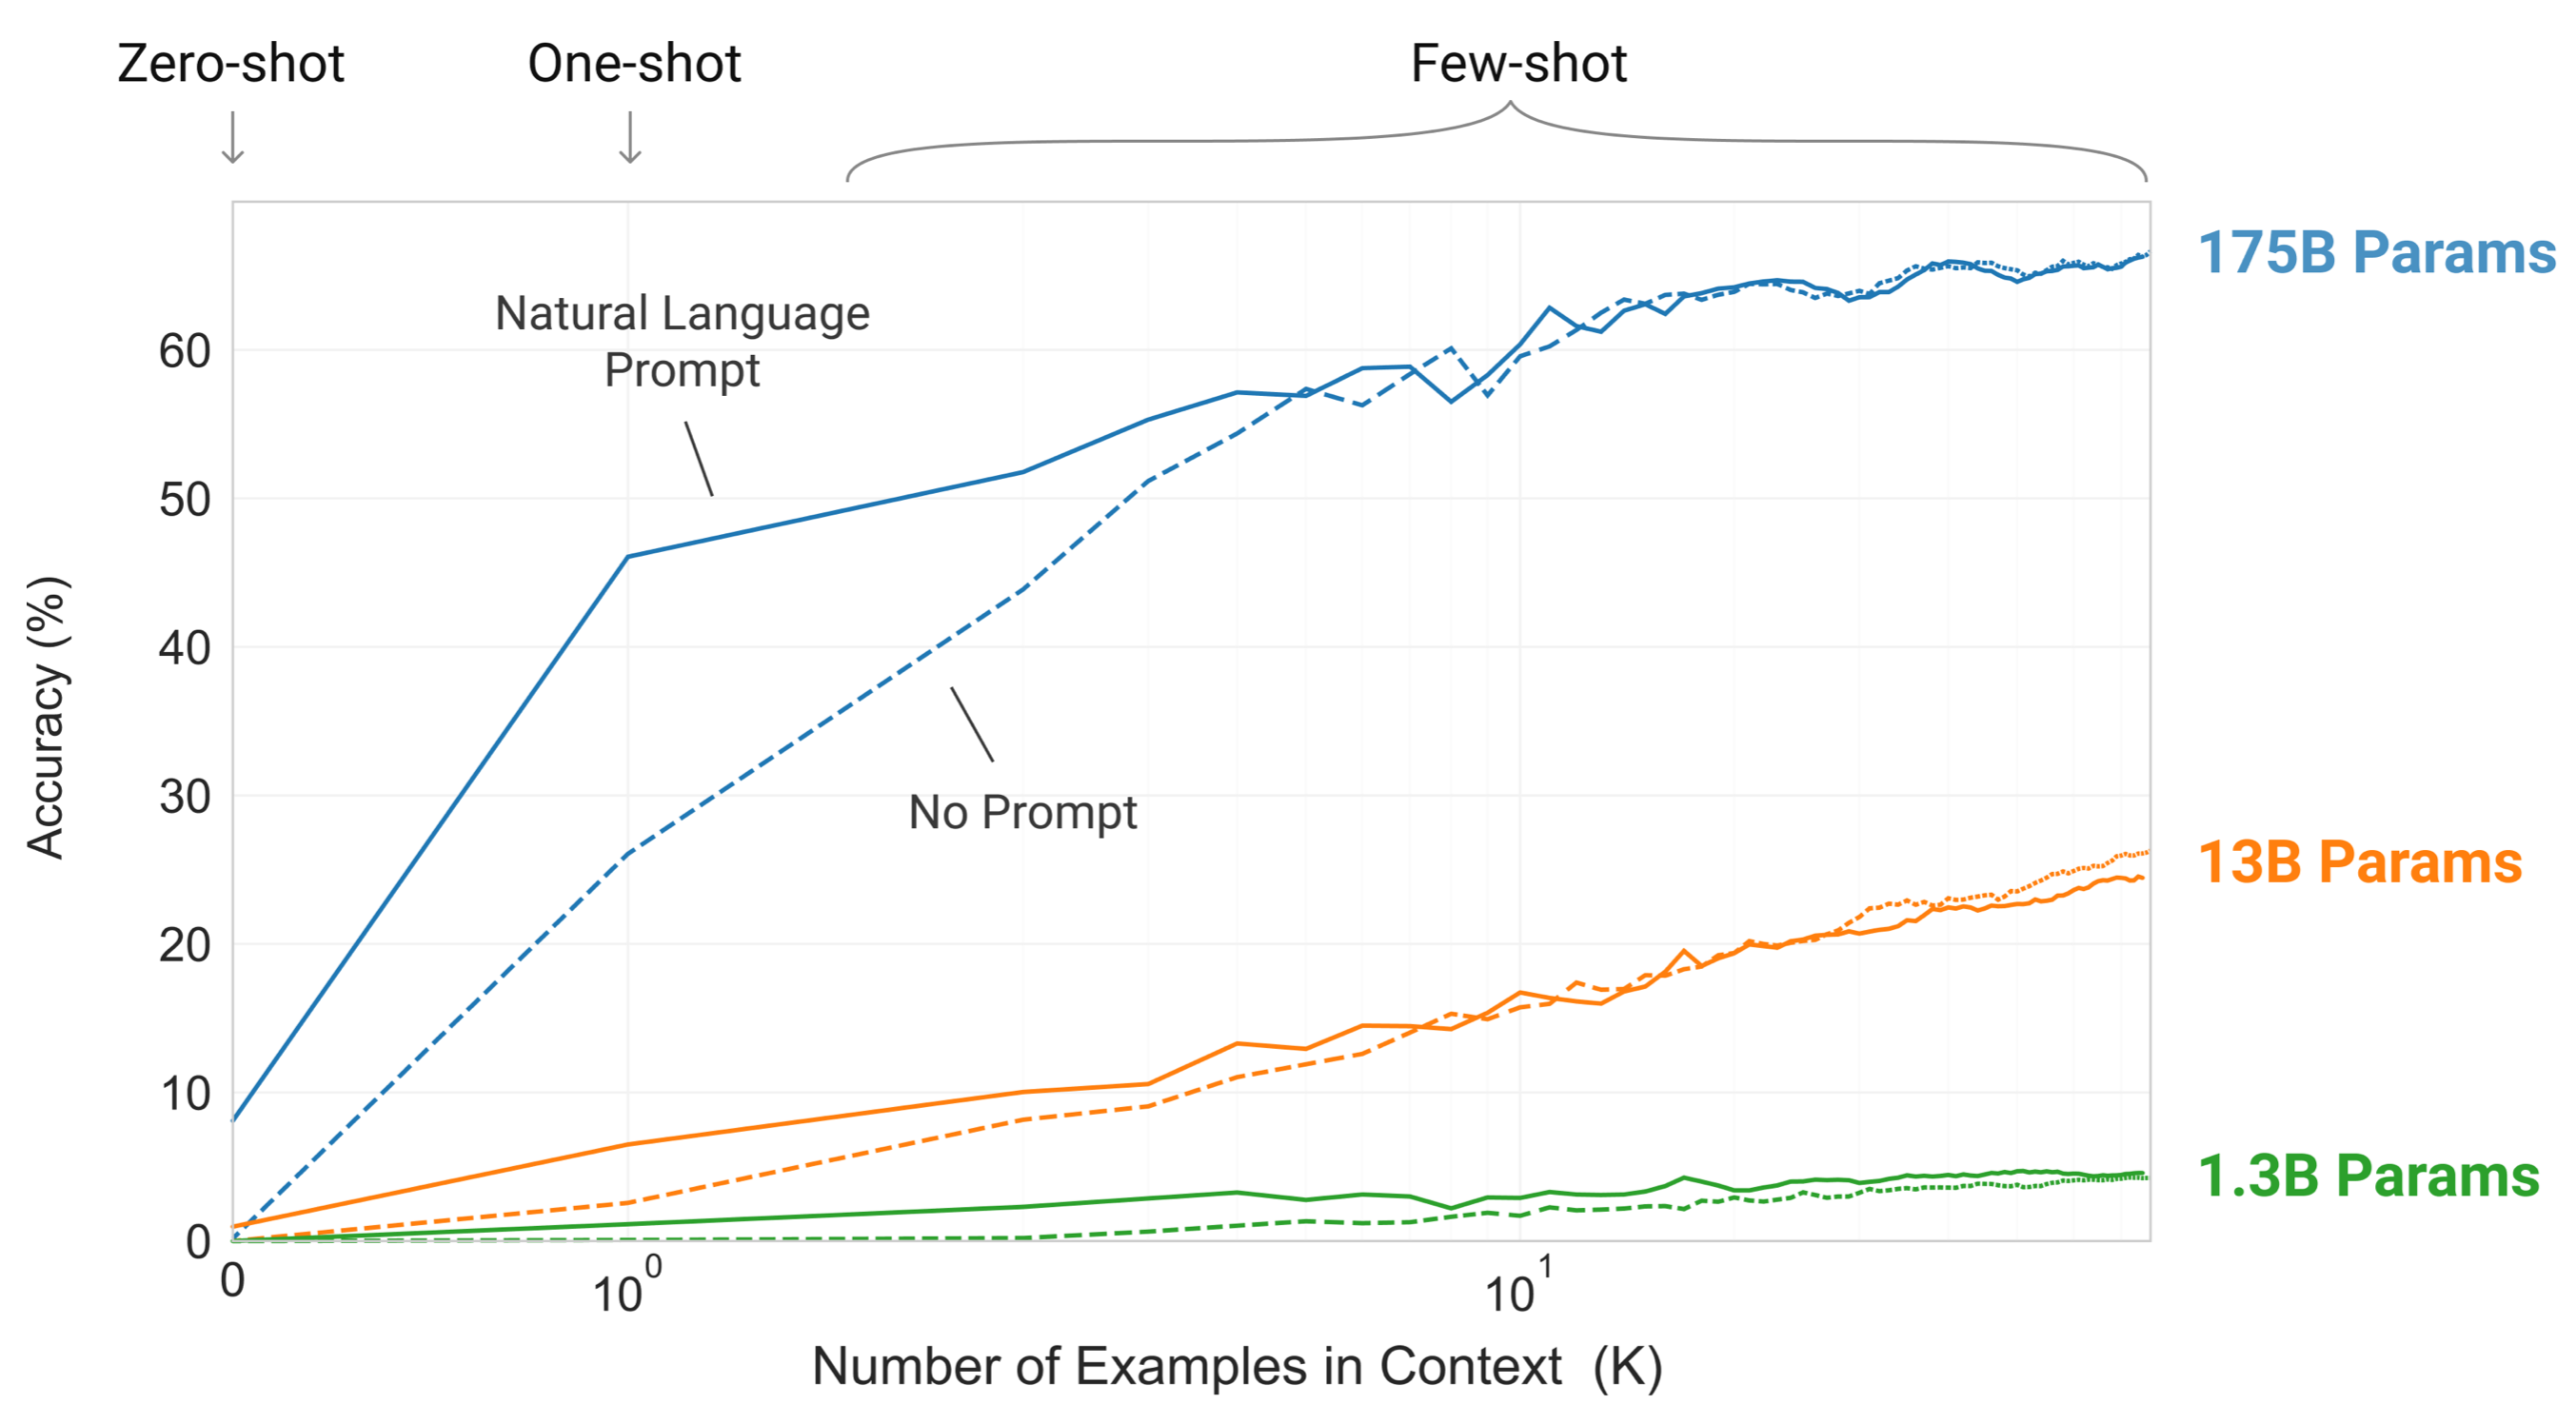
\includegraphics[width=8.50cm]{figure/incontextlearning.png}\\
		\citebutton{Source: Brown et al., 2020}{https://arxiv.org/abs/2005.14165}
\end{figure}

\begin{itemize}
	\item Number/Selection of demonstrations = Hyperparameter
	\item Larger model $\to$ Better in-context learning capabilities
\end{itemize}

\vfill

\scriptsize{*on an artificial, simple word scrambling/manipulation task}

\end{frame}

% ------------------------------------------------------------------------------

\begin{frame}{Architecture}

\vfill

\begin{itemize}
	\item Various sizes released; GPT-3 usually refers to largest one
	\item Both width ($d_{model}$) and depth ($n_{layers}$) are scaled
	\item Number of heads adjusted to $d_{model}$
\end{itemize}

	\begin{figure}
		\centering
		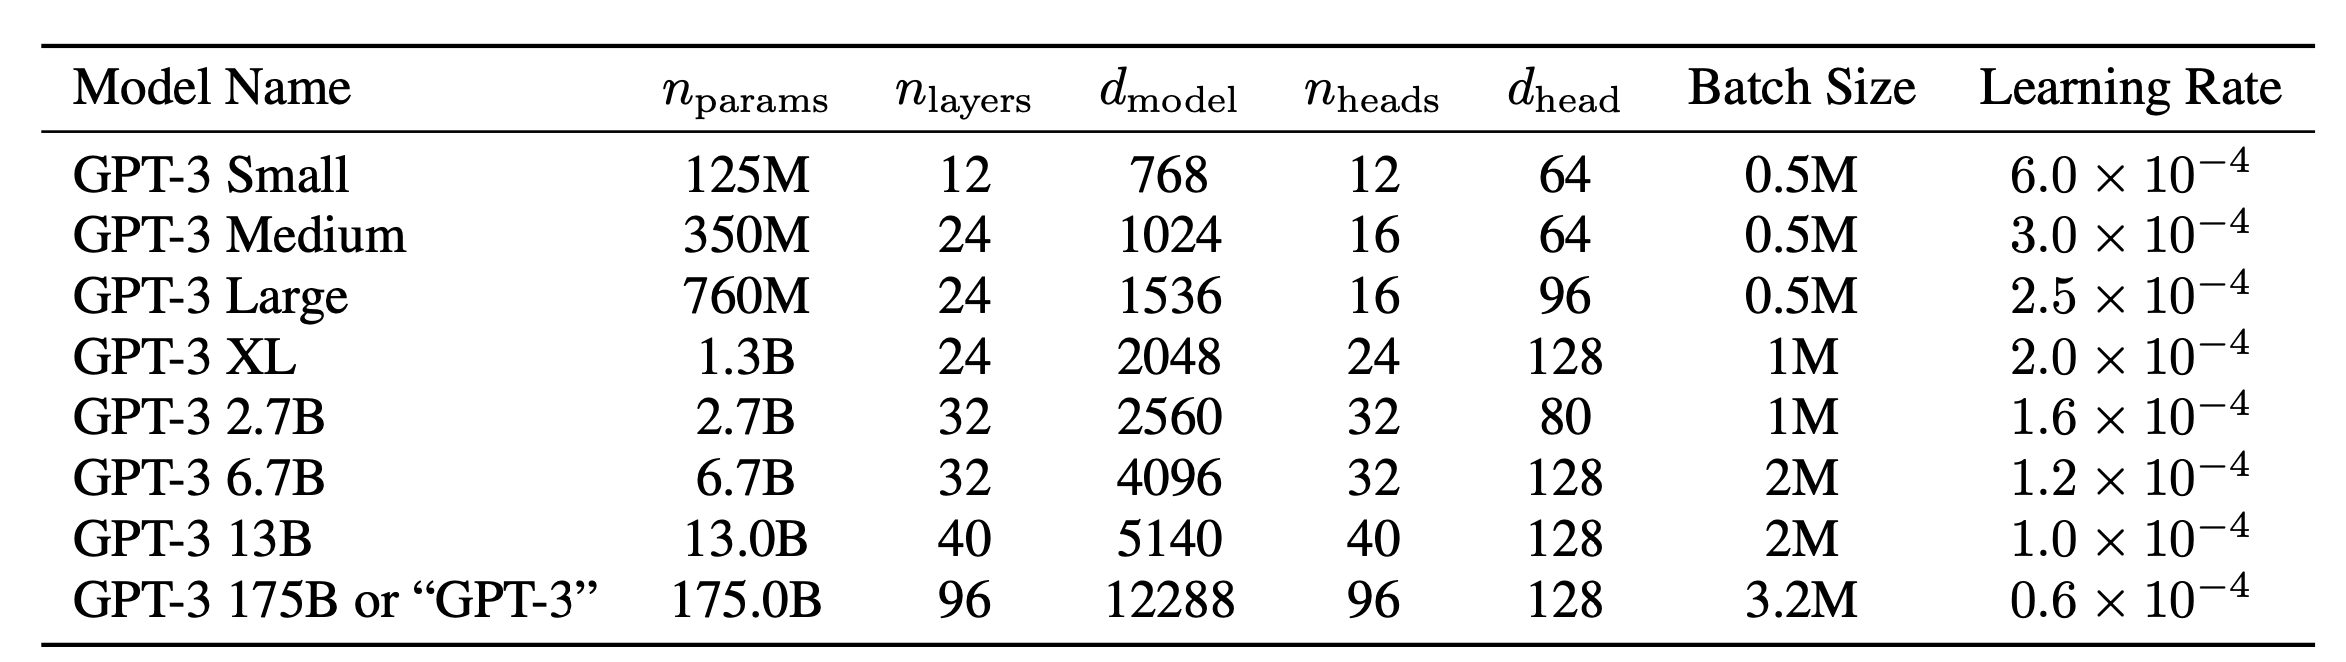
\includegraphics[width=11cm]{figure/gptarch.png}\\
		\citebutton{Source: Brown et al., 2020}{https://arxiv.org/abs/2005.14165}
	\end{figure}

\vfill

\end{frame}

% ------------------------------------------------------------------------------

\begin{frame}{X-shot comparison}
	
	\vfill
	
\begin{itemize}
	\item 42 accuracy-denominated benchmarks
	\item Few-shot performance increases faster than zero-shot
\end{itemize}

	\begin{figure}
		\centering
		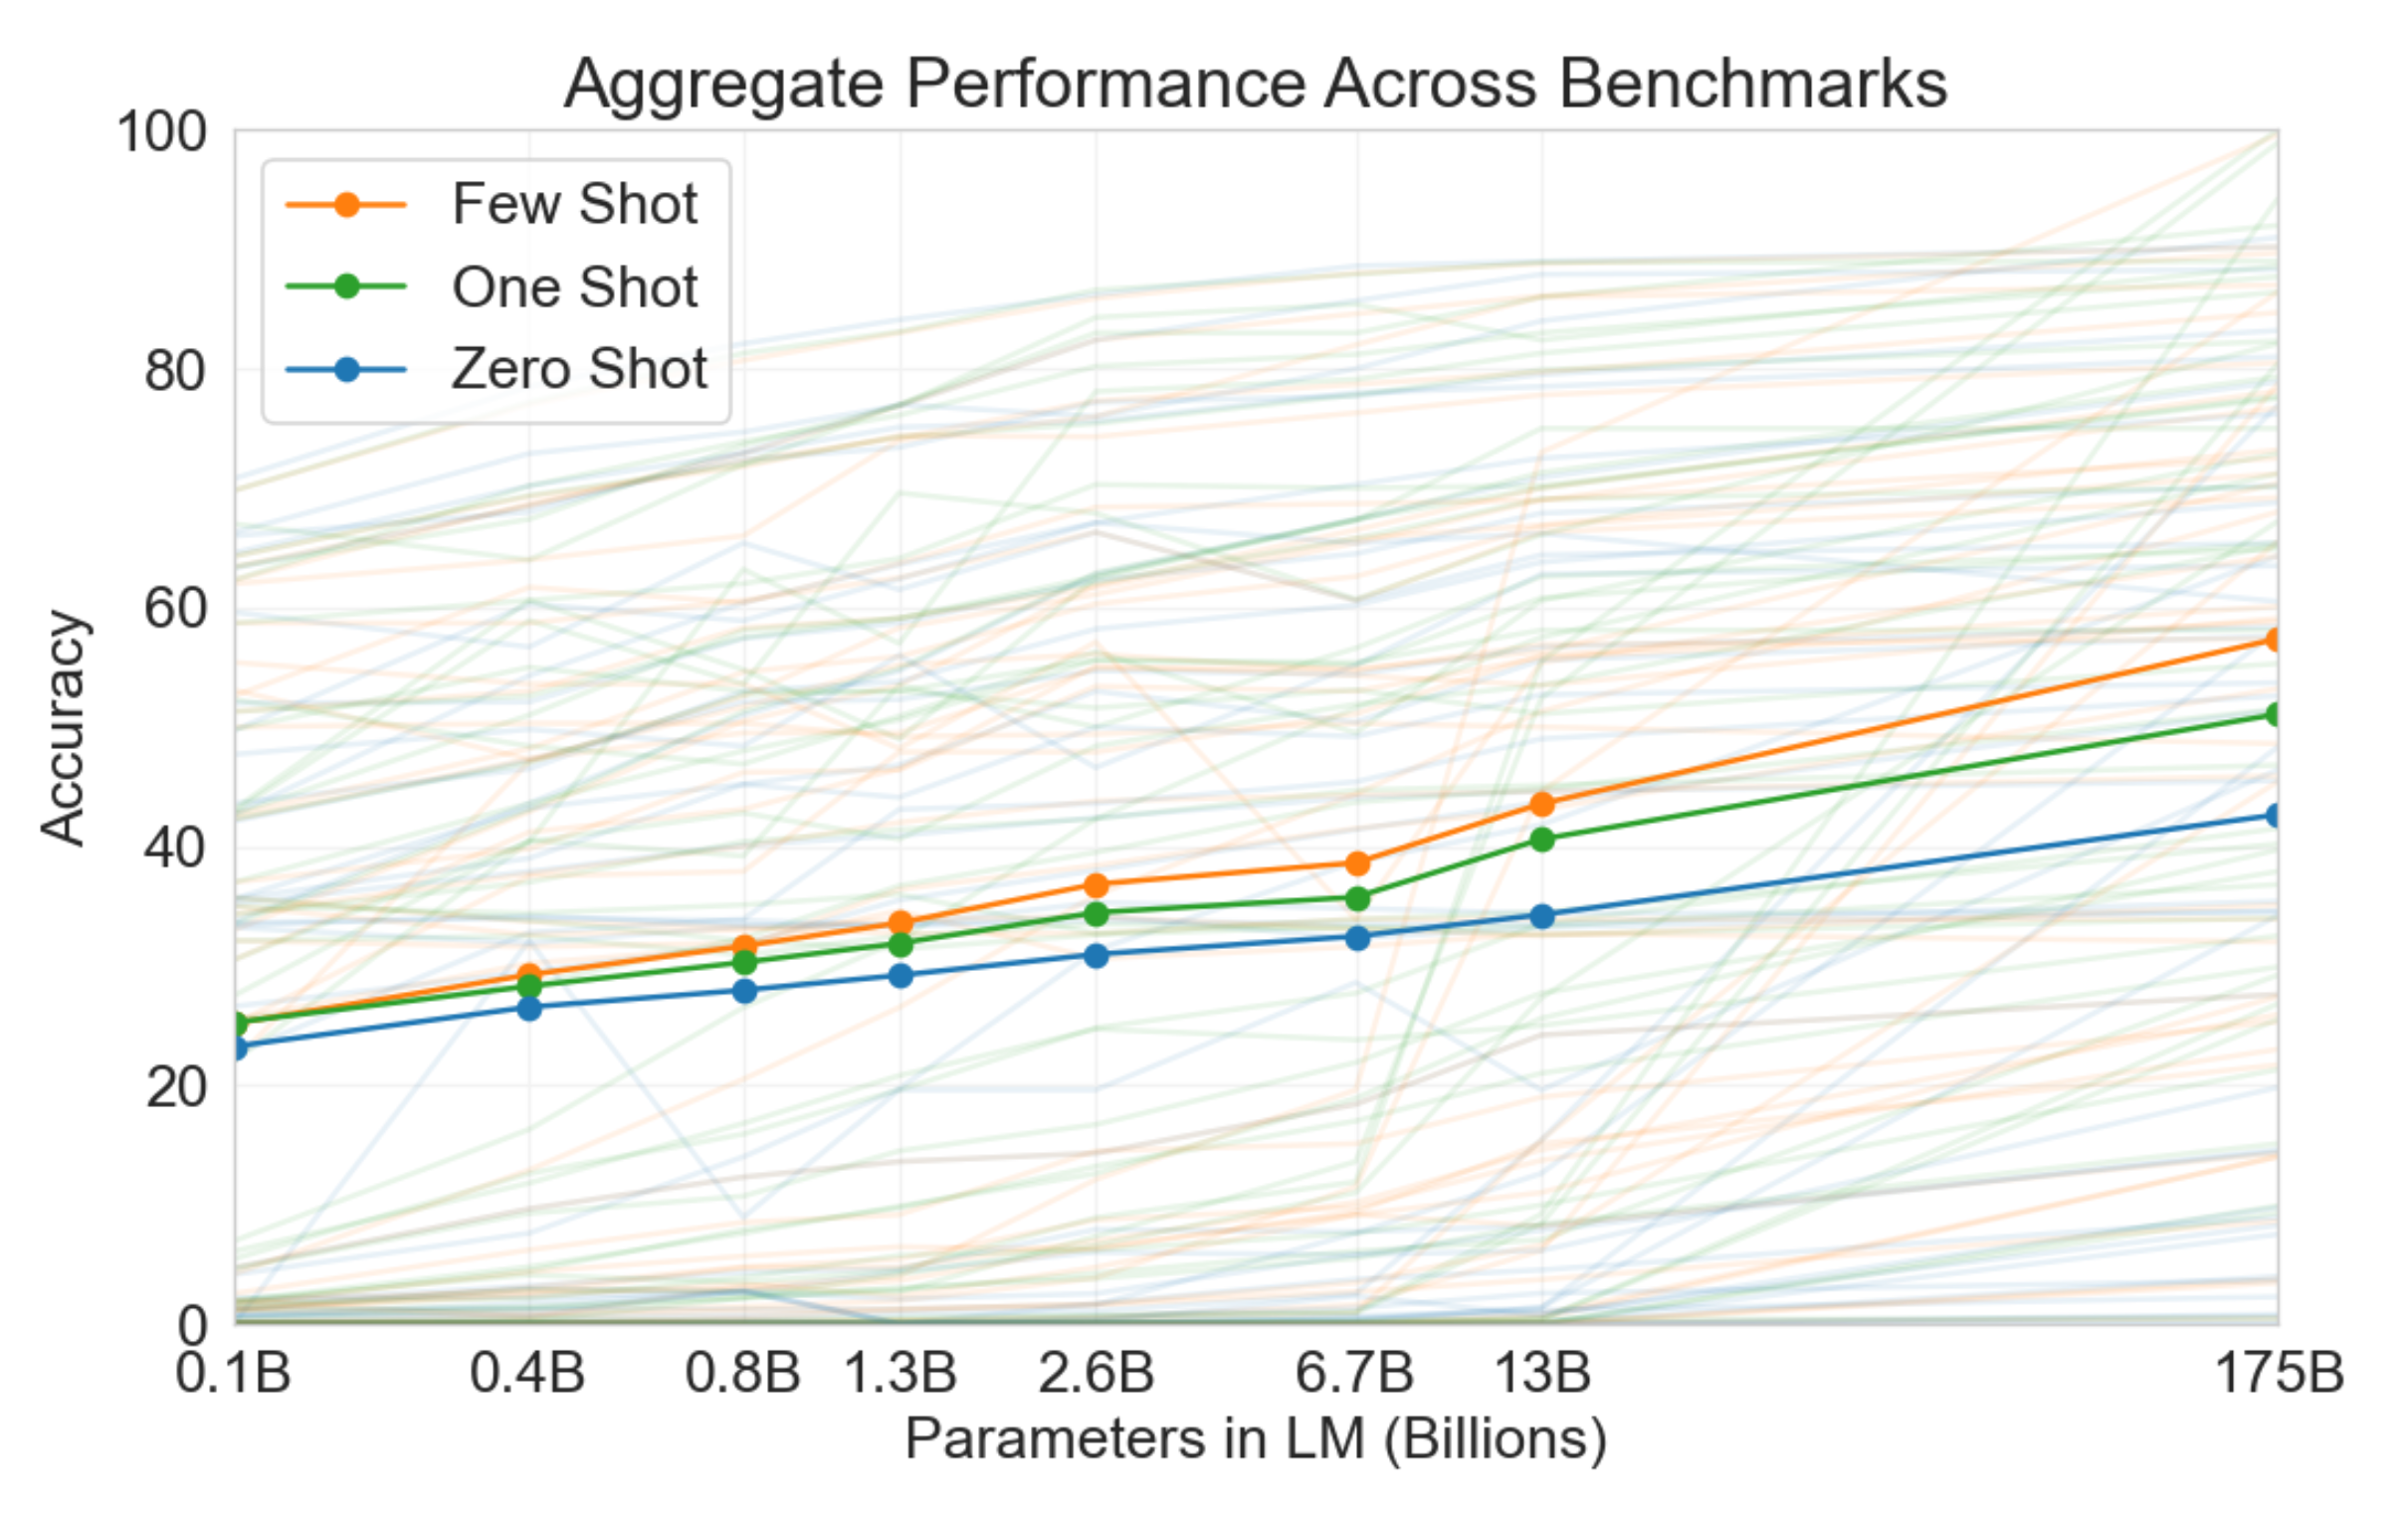
\includegraphics[width=7.65cm]{figure/xshotlargecorpora.png}\\
		\citebutton{Source: Brown et al., 2020}{https://arxiv.org/abs/2005.14165}
	\end{figure}
	
	\vfill
	
\end{frame}

%%%%%%%%%%%%%%%%%%%%%%%%%%%%%%%%%%%%%%%%%%%%%%%%%%%%%%%%%%%%%%%%%%%%
\section{Decoding}
%%%%%%%%%%%%%%%%%%%%%%%%%%%%%%%%%%%%%%%%%%%%%%%%%%%%%%%%%%%%%%%%%%%%
% Source: DL4NLP chapter08-decoding/slides-81-intro.tex

\begin{frame}{Decoding Example (1)}
\footnotesize% fit16:9


{\fontsize{8pt}{10pt}\selectfont
\noindent \textbf{Prompt:} \textcolor{blue}{Once upon a time}

\vspace{0.15cm}% fit16:9 (was 0.5cm)

\noindent \textbf{Time step 1:}
\begin{itemize}
    \item Model input: \textcolor{blue}{Once upon a time}
    \item Next token: \textcolor{red}{there}
\end{itemize}

\vspace{0.15cm}% fit16:9 (was 0.5cm)

\noindent \textbf{Time step 2:}
\begin{itemize}
    \item Model input: \textcolor{blue}{Once upon a time there}
    \item Next token: \textcolor{red}{was}
\end{itemize}

\vspace{0.15cm}% fit16:9 (was 0.5cm)

\noindent \textbf{Time step 3:}
\begin{itemize}
    \item Model input: \textcolor{blue}{Once upon a time there was}
    \item Next token: \textcolor{red}{a}
\end{itemize}

\vspace{0.15cm}% fit16:9 (was 0.5cm)

\noindent \textbf{Time step 4:}
\begin{itemize}
    \item Model input: \textcolor{blue}{Once upon a time there was a}
    \item Next token: \textcolor{red}{cat}
\end{itemize}
...
}
\end{frame}

% ------------------------------------------------------------------------------

\begin{frame}{Decoding Example (2)}

\begin{figure}
    \centering
    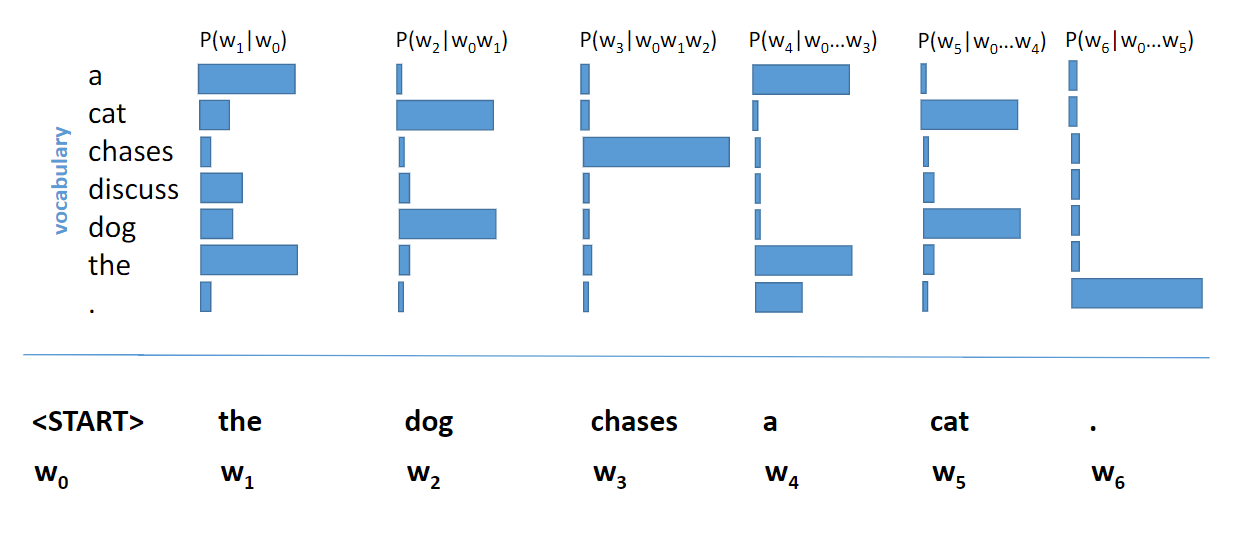
\includegraphics[width=10cm]{figure/arlm.png}
\end{figure}

\begin{itemize}
    \item At each timestep the model produces a probability distribution
    \item A decoding strategy determines how to choose the next token from that distribution, that token is then added to the context
    \item Generation stops based on stopping criteria (\textit{see: next slide})
\end{itemize}
    
\end{frame}

% ------------------------------------------------------------------------------

\begin{frame}{Stopping Criteria for Text Generations}

\vfill

\begin{itemize}
    \item \textbf{<EOS> Token}: When this token is generated the model stops
    \item \textbf{Maximum Length}: A predefined maximum length can be set for the generated text. When the text reaches this length, generation stops to prevent excessively long outputs
    \item \textbf{Maximum Time}: A predefined maximum time for generation can be set. After this time has been reached, generation stops
    \item \textbf{Other Criteria}: There are more stopping criteria implemented in huggingface \citebutton{huggingface}{https://huggingface.co/docs/transformers/internal/generation_utils\#transformers.StoppingCriteria}
\end{itemize}

\vfill

\end{frame}

% ------------------------------------------------------------------------------

\begin{frame}{Decoding Strategies}

\textbf{Deterministic}
\begin{itemize}
    \item Greedy search
    \item Beam search
    \item Contrastive search \citebutton{Su et al., 2022}{https://arxiv.org/abs/2210.14140}
    \item Contrastive decoding \citebutton{Li et al., 2023}{https://arxiv.org/abs/2210.15097}
\end{itemize}

\textbf{Stochastic}
\begin{itemize}
    \item Sampling (with temperature) 
    \item Top-$k$ sampling \citebutton{Fan et al., 2018}{https://arxiv.org/abs/1805.04833}
    \item Nucleus top-$p$ sampling \citebutton{Holtzman et al., 2019}{https://arxiv.org/abs/1904.09751}
    \item Typical sampling \citebutton{Meister et al., 2023}{https://arxiv.org/abs/2202.00666}
\end{itemize}
\vspace{1ex}

\textit{Remark:} Other decoding strategies exist, and various combinations are possible, such as top-$k$ sampling with temperature, or top-$p$ sampling followed by top-$k$ sampling (with temperature), etc.

\end{frame}

% ------------------------------------------------------------------------------

% Source: DL4NLP chapter08-decoding/slides-82-determ.tex

\begin{frame}{Greedy Search (1)}

\vfill

\begin{itemize}
    \item \textbf{Core idea}: Greedy search selects the word with the highest probability at each timestep, iteratively building the output sequence
    \item \textbf{Exploration of search space}: It explores a single path through the output space, favoring the most probable word at each step without considering future consequences
    \item \textbf{Candidate Sequence}: Only keeps track of the most likely sequence at each step, discarding other possibilities
    \item \textbf{Decision Making}: It makes local decisions based solely on the highest probability at the current step without considering potential longer-term outcomes
\end{itemize}

\vfill
    
\end{frame}

% ------------------------------------------------------------------------------

\begin{frame}{Greedy Search (2)}

\vfill

\begin{itemize}
    \item The model accepts an input sequence of tokens $x_1, x_2,...,x_N$, which we also call prompt
    \item The model then generates a token at each timestep $t$ until $T$: $y_1,y_2,...,y_T$
    \item In greedy search we choose the token with the highest conditional probability from the vocabulary V
    \item $y_t = argmax_{y \in V}P(y|y_1,y_2,...,y_{t-1},\mathbf{x})$
    \item With $y_t$ being the chosen token at timestep t and $\mathbf{x} = (x_1, x_2,...,x_N)$ being the initial prompt
\end{itemize}

\vfill

\end{frame}

% ------------------------------------------------------------------------------

\begin{frame}{Greedy Search: Example}

\begin{itemize}
    \item Suppose our vocabulary only has four tokens: $A$, $B$, $C$ and <eos>
\end{itemize}

\begin{figure}
    \centering
    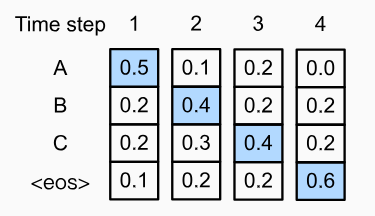
\includegraphics[width=6cm]{figure/greedy.png}\\
		\citebutton{Source: Dive Into Deep Learning Book}{https://d2l.ai/chapter_recurrent-modern/beam-search.html}
\end{figure}

\begin{itemize}
    \item At each timestep greedy search chooses the token with the highest conditional probability
    \item The model thus predicts $A$, $B$, $C$, <eos>
    \item Its probability is $0.5\cdot 0.4 \cdot 0.4 \cdot 0.6 = 0.048$
\end{itemize}

\end{frame}

% ------------------------------------------------------------------------------

\begin{frame}{Drawbacks of Greedy Search (1)}

\begin{itemize}
    \item Now we select token $C$ at timestep 2 instead of $B$
\end{itemize}

\begin{figure}
    \centering
    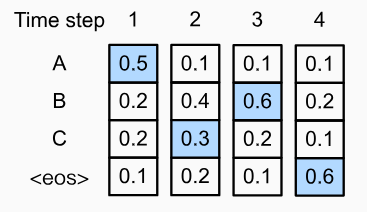
\includegraphics[width=4.33cm]{figure/greedy2.png}\\
		\citebutton{Source: Dive Into Deep Learning Book}{https://d2l.ai/chapter_recurrent-modern/beam-search.html}
\end{figure}

\begin{itemize}
    \item At the timesteps 3 and 4 the conditional probabilities change since the context is no longer $A$, $B$ but $A$, $C$
    \item The final token sequence is $A$, $C$, $B$, <eos>
    \item Its probability is $0.5 \cdot 0.3 \cdot 0.6 \cdot 0.6 = 0.054$
    \item Even though $C$ at $t=2$ has a lower probability, the final sequence has a higher probability
\end{itemize}
    
\end{frame}

% ------------------------------------------------------------------------------

\begin{frame}{Beam Search}

\vfill

\begin{itemize}
    \item \textbf{Core idea}: Beam search extends the exploration to multiple possible sequences instead of just the most probable one
    \item \textbf{Exploration of search space}: It explores multiple paths (or "beams") simultaneously, maintaining a set of promising candidate sequences
    \item \textbf{Candidate Sequence}: Keeps a fixed number of most probable sequences (determined by the beam width parameter $k$) at each step
    \item \textbf{Decision Making}: At each step, it considers multiple candidate sequences and selects the most probable ones based on their cumulative probabilities up to that point
\end{itemize}

\vfill

\end{frame}

% ------------------------------------------------------------------------------

\begin{frame}{Beam Search: Example (1)}

\vfill

\begin{itemize}
    \item Suppose $V = \{A, B, C, D, E\}$ and beam width $k=2$
\end{itemize}

\begin{figure}
    \centering
    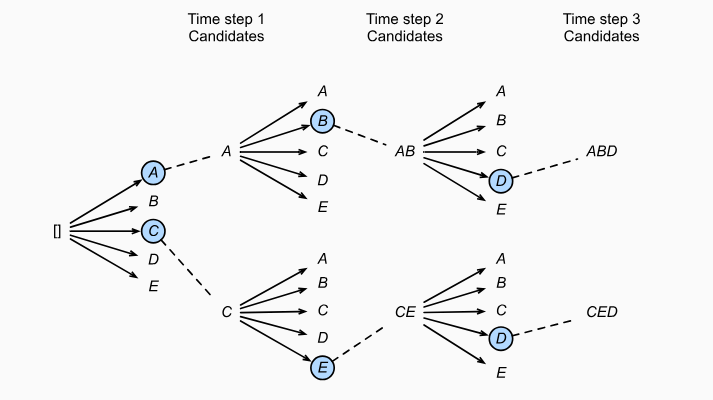
\includegraphics[width=10cm]{figure/beam.png}\\
		\citebutton{Source: Dive Into Deep Learning Book}{https://d2l.ai/chapter_recurrent-modern/beam-search.html}
\end{figure}

\vfill
    
\end{frame}

% ------------------------------------------------------------------------------

\begin{frame}{Beam Search: Example (2)}
\footnotesize% fit16:9


\vfill

\begin{itemize}
    \item At each timestep beam search chooses the $k$ tokens with the highest joint probability
    \item Suppose at $t=1$ $A$ and $C$ have the highest conditional probabilities $P(y_1|\mathbf{x})$
    \item At $t=2$ for all $y_2\in V$ we compute:
    $$
    \begin{aligned}
    P(A,y_2|\mathbf{x}) &= P(A|\mathbf{x})\cdot P(y_2|A,\mathbf{x}) \\
    P(C,y_2|\mathbf{x}) &= P(C|\mathbf{x})\cdot P(y_2|C,\mathbf{x})
    \end{aligned}
    $$
    \item And we again pick the $k$ sequences with the highest probabilities ($AB$ and $CE$)
    \item At $t=3$ again for all $y_3\in V$ we compute:
    $$
    \begin{aligned}
    P(A,B,y_2|\mathbf{x}) &= P(A,B|\mathbf{x})\cdot P(y_2|A,B,\mathbf{x}) \\
    P(C,E,y_2|\mathbf{x}) &= P(C,E|\mathbf{x})\cdot P(y_2|C,E,\mathbf{x})
    \end{aligned}
    $$
    \item We repeat this process unitl the maximum length is reached or unitl the <EOS> token gets generated
\end{itemize}

\vfill
    
\end{frame}

% ------------------------------------------------------------------------------

% Source: DL4NLP chapter08-decoding/slides-83-sampling.tex

\begin{vbframe}{Sampling Motivation}

\vfill
    
\begin{itemize}
    \item \textit{Creativity and Variation}: Sampling methods produce varied outputs for the same input, useful in creative applications like story generation and dialogue systems.
    \item \textit{Avoiding Repetition}: These methods are less likely to generate repetitive loops compared to deterministic methods.
\end{itemize}

\vfill

\end{vbframe}

% ------------------------------------------------------------------------------

\begin{vbframe}{Sampling (with temperature) (1)}



The next token is selected randomly based on its conditional probability distribution. To control the randomness of the output sequence, a temperature parameter can be applied to the softmax function

\vfill 

$$
\sigma\left(z_i\right)=\frac{e^{\frac{z_i}{temp}}}{\sum_{j=1}^N e^{\frac{z_j}{temp}}}
$$

\vfill

\begin{itemize}
\item $temp \rightarrow \infty: \text{ Output distribution $\approx$ Uniform distribution}$
\item $temp \rightarrow 0: \text{ Output distribution $\approx$ Point mass (Greedy search) }$
\end{itemize}



\end{vbframe}

% ------------------------------------------------------------------------------

\begin{vbframe}{Sampling (with temperature) (2)}

\vfill

\textbf{Prompt: "Once upon a time"}
\begin{itemize}
\item Sampling with low temperature: \textit{", during the Second World War, during the final months for his three most talented young players, the coach, Harry Gregg said this"}
\item Sampling with high temperature: \textit{"— well. Nowhere you call back my call, not on time; never the two on account my four. Do not come." This old woman — you might have liked, she herself — she did smile."}
\end{itemize}

The generated stories are diverse but sometimes very erratic.\\

\vfill

$\Rightarrow$ Sample from the top-$k$ tokens     

\end{vbframe}

% ------------------------------------------------------------------------------

\begin{vbframe}{Top-$k$ sampling \citebutton{F\MakeLowercase{an et al., 2018}}{\MakeLowercase{https://arxiv.org/abs/1805.04833}}} 


In Top-$k$ sampling, the $k$ most likely next tokens are filtered, and the probability mass is redistributed.
Visualization for $k$ = 6 in two sampling steps:

\begin{center}
    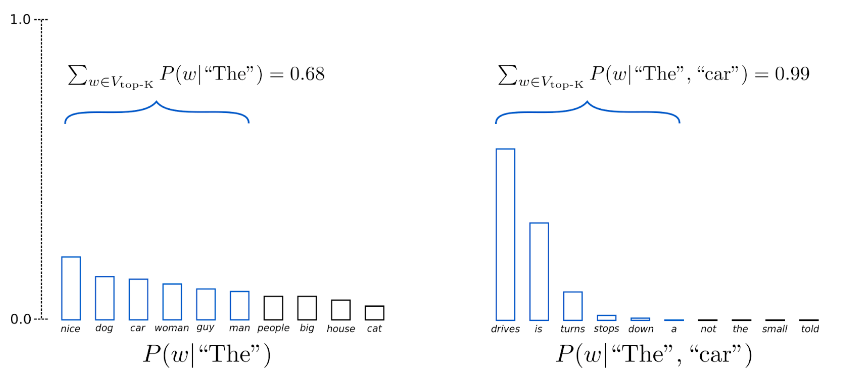
\includegraphics[width=0.9\linewidth]{figure/top_k.png}
\end{center}

\citebutton{huggingface, Patrick von Platen}{https://huggingface.co/blog/how-to-generate}

\end{vbframe}

% ------------------------------------------------------------------------------

\begin{vbframe}{Top-$k$ sampling}

\vfill

\textbf{Prompt: "Once upon a time"}
\begin{itemize}
    \item Top-$k$ , $k = 100$: \textit{"when I was young the internet was a mysterious landscape full of new and exciting ideas. I read ebooks, watched videos, read short stories"}
\end{itemize}
\vspace{2ex}

The quality has improved, but the fixed $k$ might be counterproductive\\
\vspace{2ex}
$\Rightarrow$ Make $k$ dynamic        


\end{vbframe}

% ------------------------------------------------------------------------------

\begin{frame}{Top-$p$ (Nucleus) sampling \citebutton{H\MakeLowercase{oltzman et al., 2019}}{\MakeLowercase{https://arxiv.org/abs/1904.09751}}}
% fit16:9: frame instead of vbframe, figure 0.85 (the credit line spilled onto a second page)


Top-$p$ sampling chooses from the smallest possible set of tokens whose cumulative probability exceeds the probability threshold $p$. The probability mass is then redistributed accordingly.
Visualization with a threshold $p$ = 0.92:

\begin{center}
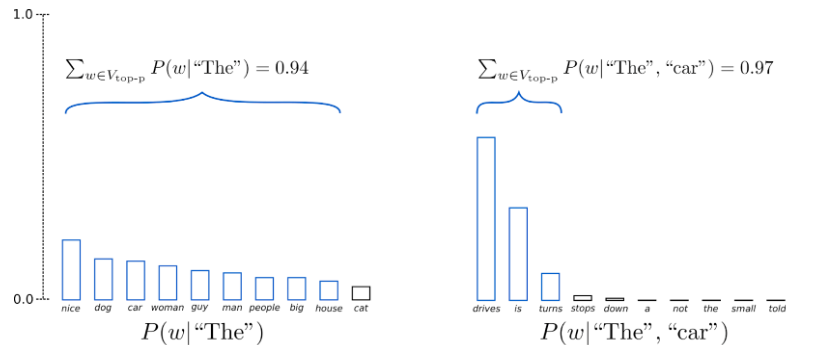
\includegraphics[width=0.85\linewidth]{figure/nucleus.png}
\end{center}

\citebutton{huggingface, Patrick von Platen}{https://huggingface.co/blog/how-to-generate}
\end{frame}

% ------------------------------------------------------------------------------

\begin{vbframe}{Top-$p$ (Nucleus) sampling}

\vfill
\textbf{Prompt: "Once upon a time"}
\begin{itemize}
    \item Top-$p$ , $p = 0.92$: \textit{"there were four major political parties in the United States. Since then, however, they have become even more of a novelty. For the past few decades, there have been only two."}
\end{itemize}

\vspace{2ex}

SOTA for many years, default decoding strategy in various GPT versions, but sometimes erratic depending on $p$ and the sampled tokens.\\

\vspace{2ex}

  
\end{vbframe}

%%%%%%%%%%%%%%%%%%%%%%%%%%%%%%%%%%%%%%%%%%%%%%%%%%%%%%%%%%%%%%%%%%%%
\section{BERT: Bidirectional Encoders}
%%%%%%%%%%%%%%%%%%%%%%%%%%%%%%%%%%%%%%%%%%%%%%%%%%%%%%%%%%%%%%%%%%%%
% Source: DL4NLP chapter04-bert/slides-41-arlm-mlm.tex  % (continued)

% [O] original bridge text (draft for the user to review); listed in order.txt
\begin{vbframe}{From GPT to BERT}
\begin{itemize}
  \item GPT predicts each token from its \emph{left} context only --- the causal mask from session 7 is what makes generation possible.
  \item For understanding tasks (classification, tagging, retrieval) the whole input is available up front; a token's meaning depends on both sides (``the \underline{bank} of the river'').
  \item Removing the causal mask gives bidirectional self-attention --- but then ``predict the next token'' becomes trivial, since the model can see it.
  \item BERT's answer: hide some tokens and predict them from both sides --- the \textbf{masked language model} objective.
\end{itemize}
\end{vbframe}
\begin{frame}{Masked language models (MLM)}

\vfill

\begin{itemize}
	\item We have seen auto-regressive LMs
			\begin{itemize}
				\item context: previous words
				\item predict: next word
			\end{itemize}
	\item Another type: \textit{Masked} LMs (MLMs)
			\begin{itemize}
				\item context: surrounding words
				\item predict: masked word
			\end{itemize}
\end{itemize}

\vfill

\end{frame}

% ------------------------------------------------------------------------------

\begin{frame}{mlm: toy example}

\vfill

	\begin{figure}
		\centering
		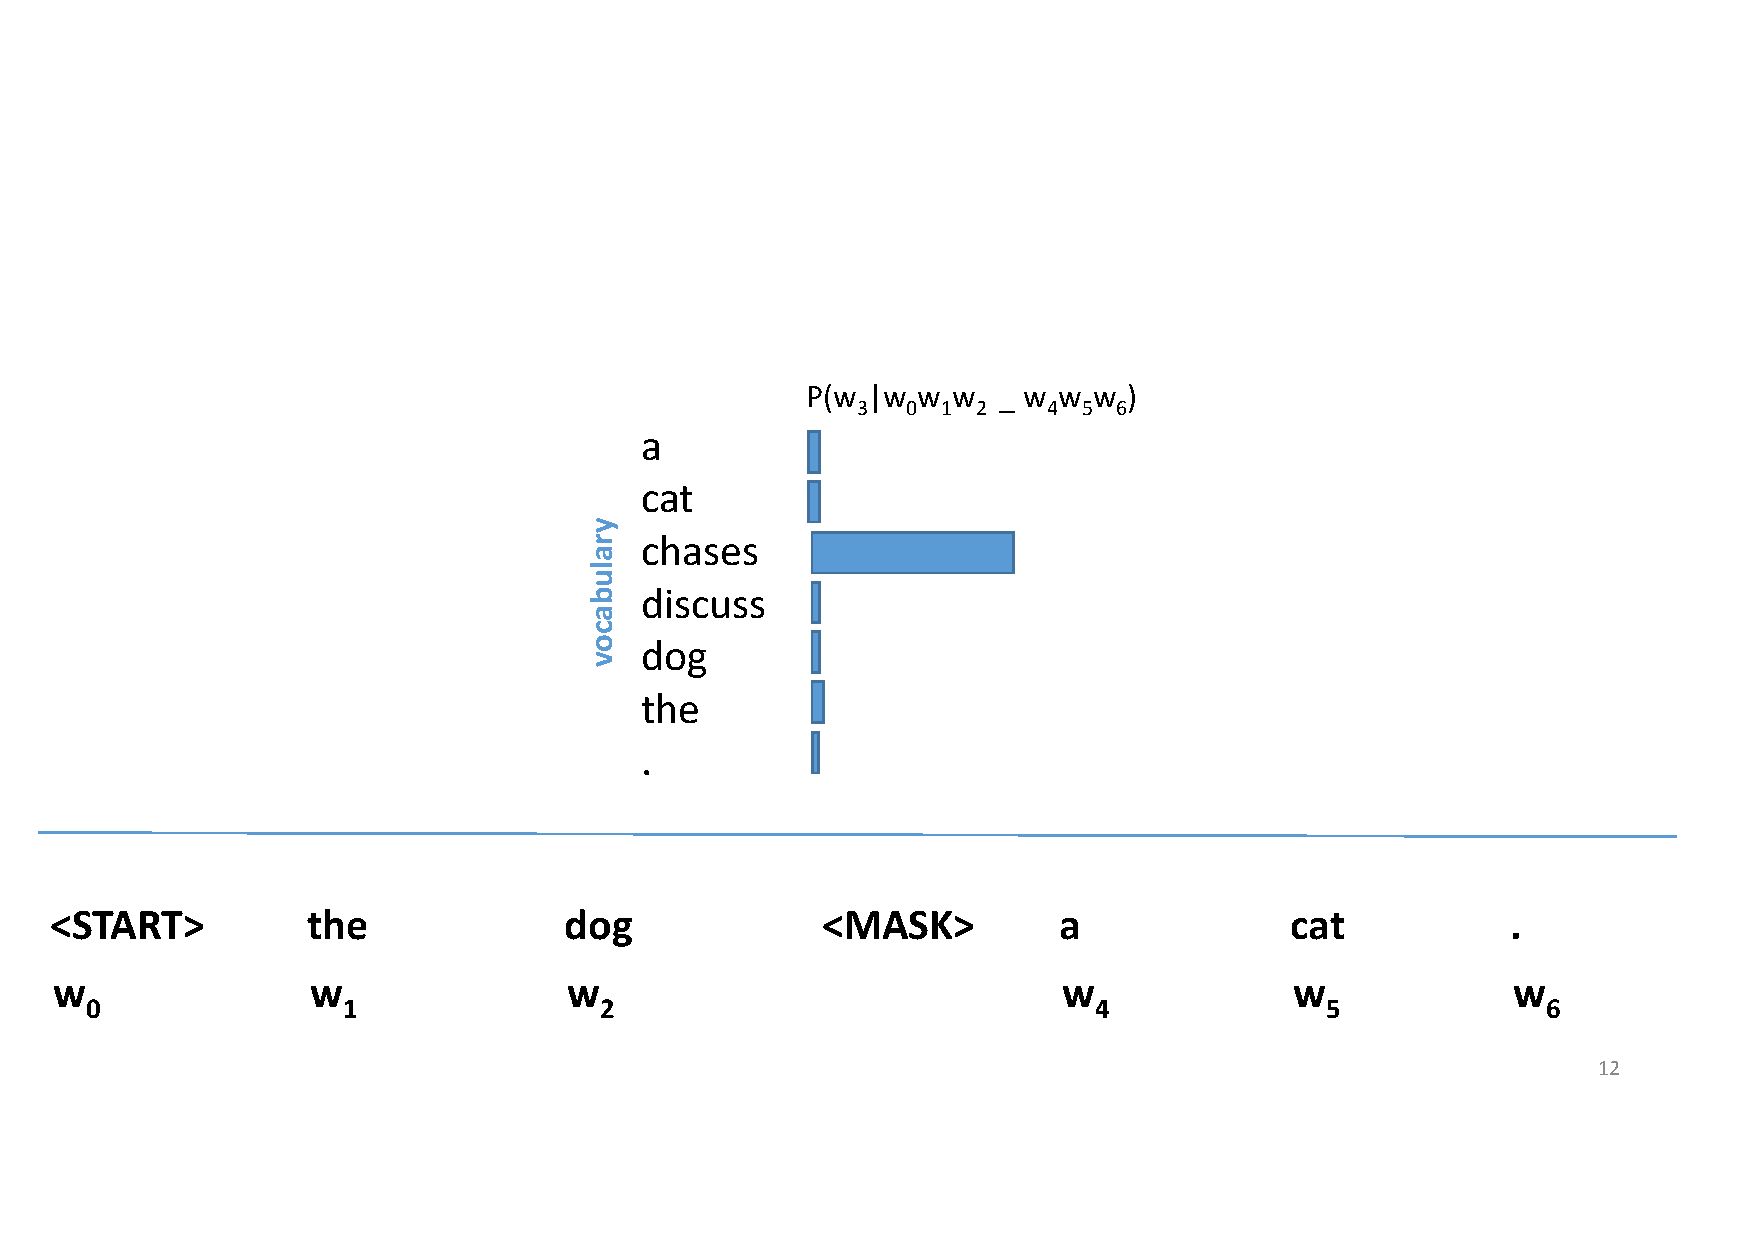
\includegraphics[width=8.50cm]{figure/mlm.pdf}
	\end{figure}
	
\vfill

\end{frame}

% ------------------------------------------------------------------------------

\begin{frame}{mlm: probabilistic interpretation}

\vfill

\begin{itemize}
	\item Estimates $P(w_i | w_0, w_1, w_{i-1}, \dots, w_{i+1}, w_n)$
	\item No ``clean`` estimate for $P(sentence)$, as
	$$ P(w_1, w_2, \dots, w_n | w_0)$$ $$\neq P(w_1 | w_0, w_2, \dots, w_n) \cdot P(w_2 | w_0, w_1, w_3, \dots, w_n)$$
	\item ARLMs are better than MLMs for generating texts 
	\item Advantage of MLMs: Learning contextualized representations
\end{itemize}

\vfill

\end{frame}

% ------------------------------------------------------------------------------

% Source: DL4NLP chapter04-bert/slides-43-corefacts.tex

\begin{frame}{bert: key facts}

\vfill

\textit{\textbf{B}idirectional \textbf{E}ncoder \textbf{R}epresentations from \textbf{T}ransformers:}

\vspace{.5cm}

\begin{itemize}
		\item Bidirectionally contextual model\\
					$\to$ The embeddings of a single token depend on its left- and on its right-side context (similar to ELMo, but better)
		\item Completely replaces recurrent architectures by Self-Attention\\
					$\to$ parallelizable
		\item Model can be fine-tuned as a whole
\end{itemize}

\vfill

\end{frame}

% ------------------------------------------------------------------------------

% Excursus added on request (ELMo is referenced above but not covered in this deck).
% Bullets verbatim from DL4NLP chapter02-deeplearningbasics/slides-23-elmo.tex
% (frames "embeddings from language models", "ELMo embeddings", "Summary").

\begin{frame}{Excursus: ELMo}

\vfill

\textit{\textbf{E}mbeddings from \textbf{L}anguage \textbf{Mo}dels}
\beamergotobutton{\href{https://aclanthology.org/N18-1202/}{Peters et al., 2018}}

\vspace{.5cm}

	\begin{itemize}
		\item Bidirectional language model (LM)
		\item Combines a forward LM and a backward LM
		\item Two-layer biLSTM as main architecture
	\end{itemize}

	\textbf{Summary:}

	\begin{itemize}
		\item Embeddings are (bidirectionally!) contextualized \\
					(as opposed to word2vec)
		\item Embeddings are \textit{not} adapted to target domain/task \\
					(similar as for word2vec)
		\item Additional weights are learned for each downstream task \\
					(i.e. besides the embeddings, no shared knowledge across tasks)
	\end{itemize}

\vfill

\end{frame}

% ------------------------------------------------------------------------------

\begin{frame}{bert: key facts}

\vfill

	\begin{itemize}
		\item New self-supervised objective(s)
		\item[] $\to$ MLM as \textit{necessity} for the architecture to work
		\item[] $\to$ Next-Sentence-Prediction as complementary objective
		\item Transformer \textit{encoder} as backbone of the architecture
		\item 110M (340M) parameters in total for $BERT_{Base}$ ($BERT_{Large}$)
			\begin{itemize}
				\item 12 (24) Transformer encoder blocks
				\item Embedding size of $E = 768$ (1024)
				\item Hidden layer size $H = E$
				\item $A = H/64 = 12$ (16) attention heads
				\item Feed-forward size is set to $4H$
			\end{itemize}
	\end{itemize}

\vfill

\end{frame}

% ------------------------------------------------------------------------------

\begin{frame}{Core of BERT -- Transformer Encoder}

\begin{figure}
	\centering
		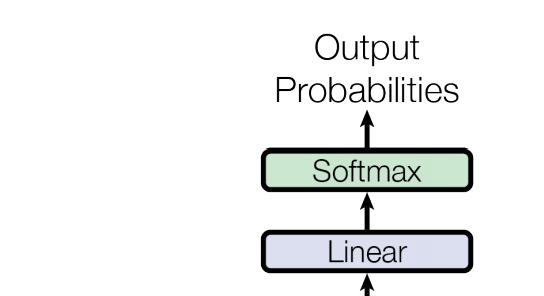
\includegraphics[width = 2.55cm]{figure/bert-top.png}\\ 
		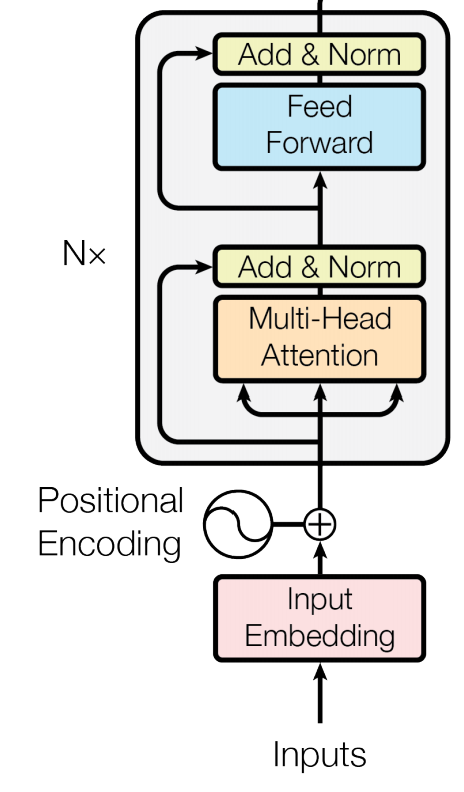
\includegraphics[width = 2.38cm]{figure/bert-bottom.png}\\ 
	\citebutton{Vaswani et al. (2017)}{https://arxiv.org/pdf/1706.03762.pdf}
\end{figure}

\end{frame}

% ------------------------------------------------------------------------------

\begin{frame}{A remark on "Causality"}

\vfill

\textbf{Causality is an issue!}
	
\begin{itemize}
	\item Goal: Learn contextual representations for words/tokens
	\item \textit{Self-Supervision:} Input and target sequence are the same\\
				$\rightarrow$ We modify the input to create a meaningful task 
	\item \warning Unconstrained Self-Attention makes using the LM objective infeasible
	\item \ques Why is this the case?
	\pause
	\item[] Bidirectionality at a lower layer would allow a word to see itself at later hidden layers\\
				$\rightarrow$ The model would be allowed to cheat!\\
				$\rightarrow$ This would not lead to meaningful internal representations
\end{itemize}

\vfill

\end{frame}

% ------------------------------------------------------------------------------

\begin{frame}{bert -- input embeddings}

\vfill

\begin{figure}
	\centering
	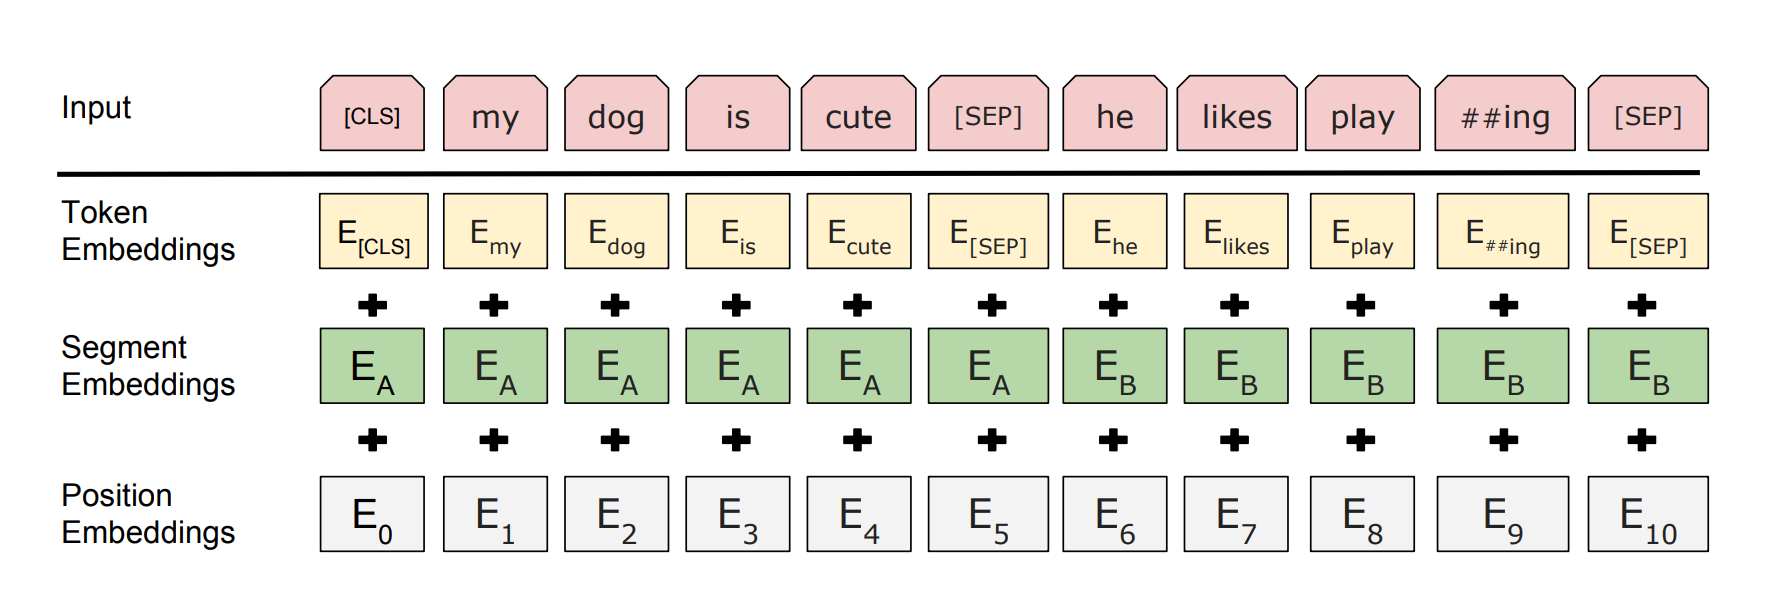
\includegraphics[width = 10cm]{figure/bert-input.png}\\ 
	\citebutton{Source: Devlin et al., 2019}{https://aclanthology.org/N19-1423.pdf}
\end{figure}

\begin{itemize}
	\item Two concatenated sentences as input
	\item WordPiece tokenization \citebutton{Wu et al., 2016}{https://arxiv.org/abs/1609.08144} for the inputs\\
			$\rightarrow$ Vocabulary of 30.000 tokens
	\item \textit{Learned} segment $+$ position embeddings
	\item Special \texttt{[CLS]} and \texttt{[SEP]} tokens
\end{itemize}

\vfill

\end{frame}

% ------------------------------------------------------------------------------

\begin{frame}{bert -- all embeddings}

\vfill

\begin{figure}
	\centering
	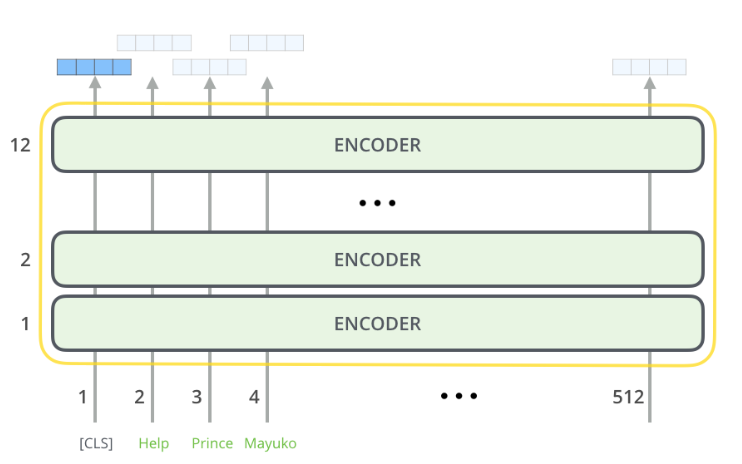
\includegraphics[width = 6.80cm]{figure/bert-embedings.png}\\ 
		\citebutton{Source: Jay Alammar}{https://jalammar.github.io/illustrated-bert/}
\end{figure}

\begin{itemize}
	\item One embedding per token per layer
	\item Non-contextual embeddings in the very first embedding layer
	\item More contextualization deeper into the model
\end{itemize}

\vfill

\end{frame}

% ------------------------------------------------------------------------------

\begin{frame}{bert -- the role of [CLS] and [SEP]}

\vfill

\textbf{Why deliberately include extra ``words``?}

\begin{itemize}
	\item The \texttt{[CLS]} token serves as an overall embedding for representing the whole sequence\\
				$\to$ Later on BERT can thus used for classifying whole sequences\\
				$\to$ Can be extracted and used for clustering or similar
	\item The \texttt{[SEP]} (short for ```separator`) token serves as a ``signal`` for the model when used for taks on pairs of sequences
\end{itemize}

\textbf{Note:}

\begin{itemize}
	\item One further ``special`` token: \texttt{[UNK]} for representing unknown tokens or symbols (so the don't ``break`` the model)
\end{itemize}

\vfill

\end{frame}

% ------------------------------------------------------------------------------

\begin{frame}{Two different BERT versions}
\textit{There are two different BERT versions, namely BERT base and large. Depending on the architecture we get different parameter counts} \citebutton{Source: Devlin et al., 2019}{https://arxiv.org/abs/1810.04805}

\begin{itemize}
	\item \textbf{BERT base:}
	\begin{itemize}
		\item $n_{layers} = 12$, we have 12 encoder layers
		\item $n_{heads} = 12$, this will not affect the parameter count since they perfectly split $d_{model}$ across the heads
		\item $d_{model} = 768$, thats the embedding dimension
	\end{itemize}

	\item \textbf{BERT large:}
	\begin{itemize}
		\item $n_{layers} = 24$
		\item $n_{heads} = 16$
		\item $d_{model} = 1024$
	\end{itemize}
\end{itemize}
	
\end{frame}

% ------------------------------------------------------------------------------

% Source: DL4NLP chapter04-bert/slides-44-pretrain-finetune.tex

\begin{frame}{Masked Language Modeling (MLM)}

\vfill

\textbf{First remark:}

\begin{itemize}
	\item Distinguish from \textit{Masked Self-Attention}\\ 
				$\to$ Masked Self-Attention is an architectural detail in the decoder of the Transformer, i.e. used by e.g. GPT
	\item Masked Self-Attention as a way to prevent causality issues in a Transformer decoder 
	\item MLM is a self-supervised \textit{modeling objective} introduced to couple Self-Attention and (deep) bidirectionality without violating causality
\end{itemize}

\vfill

\end{frame}

% ------------------------------------------------------------------------------

\begin{frame}{MLM (2)}

\begin{itemize}
\item \textbf{Training objective:} $$\text{Given a sentence, predict \texttt{[MASK]}ed tokens}$$
\item \textbf{Generation of samples:} $$\text{Randomly replace* a fraction of the words by \texttt{[MASK]}}$$
  \scriptsize *Sample 15\% of the tokens; replace 80\% of them by \texttt{[MASK]}, 10\% by a random token \& leave 10\% unchanged
\item \normalsize \textbf{Input:}\\\mbox{}\\
			\footnotesize
\begin{tabular}{|cccccccccc|}
\hline
The & quick & brown & \cellcolor{blue!65}\texttt{[MASK]} & jumps & over & the & \cellcolor{blue!65}\texttt{[MASK]} & dog & . \\
\hline
\end{tabular}\\\mbox{}
\item \normalsize \textbf{Targets:} $$(fox,\; lazy)$$
\end{itemize}

\end{frame}

% ------------------------------------------------------------------------------

\begin{frame}{MLM (3)}

\begin{itemize}
\item \warning But 20\% of the samples will look different!\\
			$\to$ 10\% replaced by a random token; 10\% left unchanged
\item \normalsize \textbf{Input (first case):}\\\mbox{}\\
			\footnotesize
\begin{tabular}{|cccccccccc|}
\hline
The & quick & brown & \cellcolor{blue!65}\texttt{orange} & jumps & over & the & \cellcolor{blue!65}\texttt{is} & dog & . \\
\hline
\end{tabular}\\\mbox{}
\item \normalsize \textbf{Targets (first case):} $$(fox,\; lazy)$$
\item \normalsize \textbf{Input (second case):}\\\mbox{}\\
			\footnotesize
\begin{tabular}{|cccccccccc|}
\hline
The & quick & brown & \cellcolor{blue!65}\texttt{fox} & jumps & over & the & \cellcolor{blue!65}\texttt{lazy} & dog & . \\
\hline
\end{tabular}\\\mbox{}
\item \normalsize \textbf{Targets (second case):} $$(fox,\; lazy)$$
\end{itemize}

\end{frame}

% ------------------------------------------------------------------------------

\begin{frame}{MLM (4)}

\vfill

\textbf{Discrepancy between pre-training \& fine-tuning:}

\begin{itemize}
	\item \texttt{[MASK]}-token as central part of pre-training procedure
	\item \texttt{[MASK]}-token does not occur during fine-tuning
	\item \textbf{Modified pre-training task:}\\
				Predict 15\% of the tokens of which only 80\% have been replaced by \texttt{[MASK]}
				\begin{itemize}
					\item 80\% of the selected tokens are actually \texttt{[MASK]}ed
					\item 10\% of the selected tokens: The model has to ``understand`` that the word needs to be \textit{replaced}
					\item 10\% of the selected tokens: The model has to ``understand`` that the word needs to be \textit{kept}
			\end{itemize}
	\item This ensures overlap between the kind data seen during pre-training and during fine-tuning
\end{itemize}
	
\vfill

\end{frame}

% ------------------------------------------------------------------------------

\begin{frame}{MLM (5)}

\vfill

	\begin{figure}
		\centering
		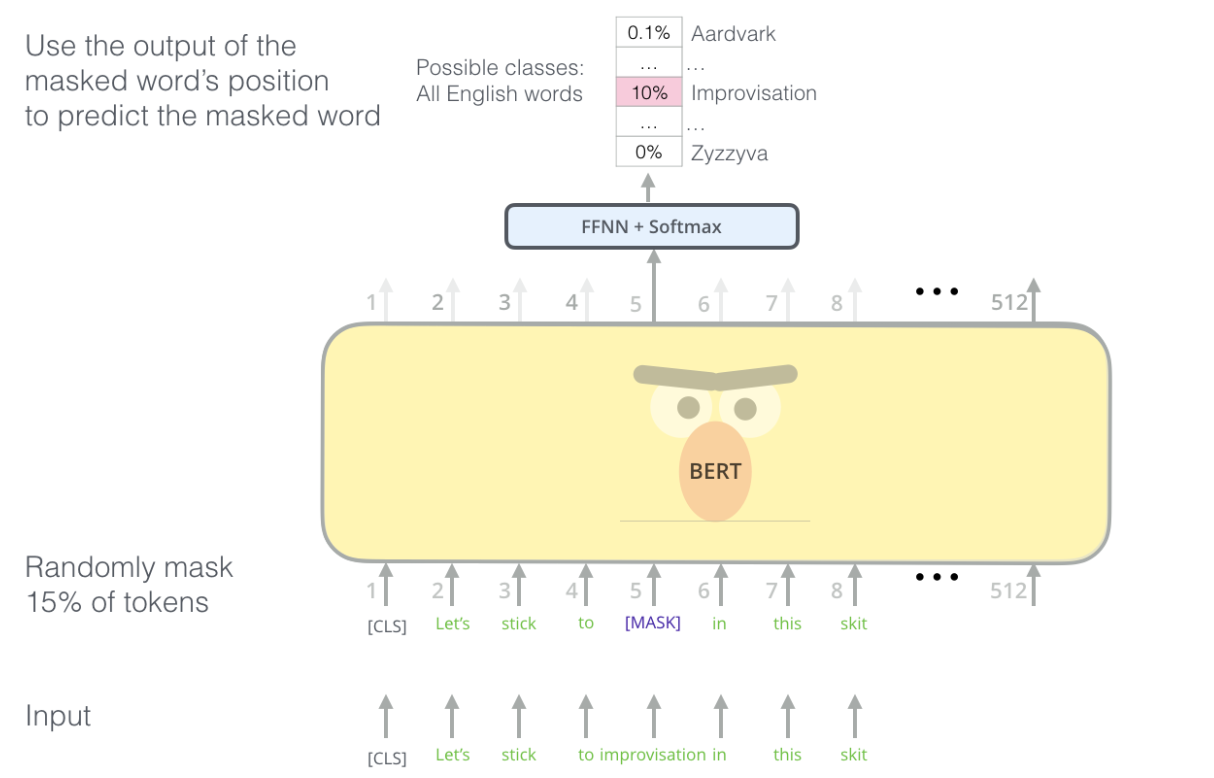
\includegraphics[width = 8.50cm]{figure/bert-mlm.png}\\ 
		\citebutton{Source: Jay Alammar}{https://jalammar.github.io/illustrated-bert/}
	\end{figure}

\vfill

\end{frame}

% ------------------------------------------------------------------------------

\begin{frame}{Next Sentence Prediction (NSP)}

\begin{itemize}
\item \textbf{Training objective:} $$\text{Given two sentences, predict whether $s_2$ follows $s_1$}$$
\item \textbf{Generation of samples:} $$\text{Randomly sample* negative examples}$$
  \scriptsize *50\% of the time the second sentence is the actual next sentence, 50\% of the time it is a randomly sampled sentence
\item \normalsize \textbf{Full Input:}\\\mbox{}\\
			\footnotesize
\begin{center}
\begin{tabular}{|cccccccc|}
\hline
\cellcolor{blue!15}\texttt{[CLS]} & The & \cellcolor{blue!65}\texttt{[MASK]} & is & quick & . & \cellcolor{blue!15}\texttt{[SEP]} &\\\hline\hline It & jumps & over & the & \cellcolor{blue!65}\texttt{[MASK]} & dog & . & \cellcolor{blue!15}\texttt{[SEP]} \\
\hline
\end{tabular}\\\mbox{}
\end{center}
\item \normalsize \texttt{[CLS]} token as sequence representation for classification
\item \texttt{[SEP]} token for separation of the two input sequences
\end{itemize}

\end{frame}

% ------------------------------------------------------------------------------

\begin{frame}{NSP (2)}

\vfill

	\begin{figure}
		\centering
		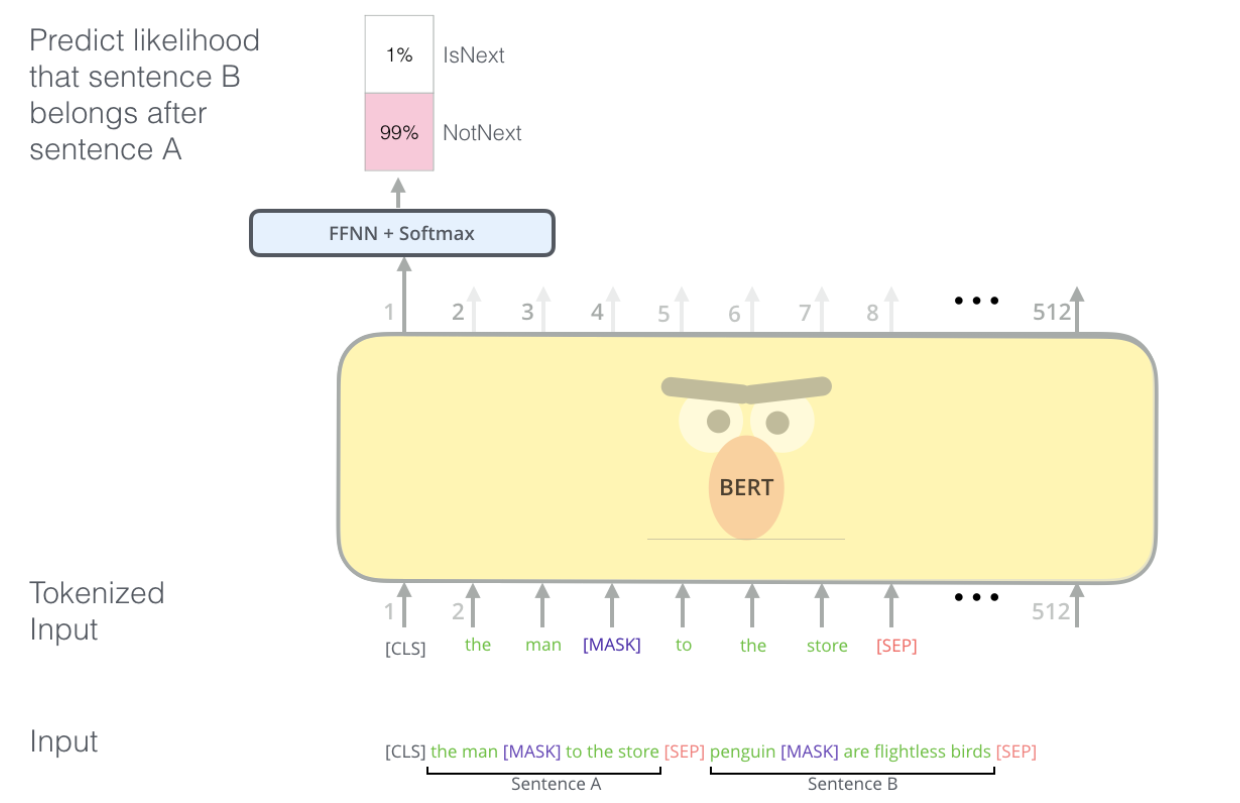
\includegraphics[width = 8.50cm]{figure/bert-nsp.png}\\ 
		\citebutton{Source: Jay Alammar}{https://jalammar.github.io/illustrated-bert/}
	\end{figure}

\vfill

\end{frame}

% ------------------------------------------------------------------------------

\begin{frame}{Pre-Training BERT}

\vfill

\textbf{Setup:}

\begin{itemize}
	\item 13 GB of text (BooksCorpus $+$ Eng. Wikipedia)\\
				$\rightarrow$ Back then: \textbf{huge}; Now: rather \textbf{small}
	\item Train for approximately* 40 epochs
	\item 4 (16) \href{https://cloud.google.com/tpu/}{Cloud TPUs} for 4 days for the BASE (LARGE) variant
	\item Loss function: $$Loss_{BERT} = Loss_{MLM} + Loss_{NSP}$$
\end{itemize}

\vfill

{\scriptsize *1.000.000 steps on batches of 256 sequences with a sequence length of 512 tokens}
\end{frame}

% ------------------------------------------------------------------------------

\begin{frame}{Pre-Training BERT}

\vfill

\textbf{Sequence lengths:}

\begin{itemize}
	\item For their experiments:
		\begin{itemize}
			\item Pre-train w/ sequence length 128 for 90\% of the steps
			\item Pre-train w/ sequence length 512 for 10\% of the steps \\
		\end{itemize}
	\item \textit{Reason:} Positional embeddings
		\begin{itemize}
			\item Learned, not sinusoidal (as opposed to the original Transformer)
			\item Training on long sequences necessary to learn them well
			\item \textbf{But:} Training expensive, hence this ``compromise``
		\end{itemize}
\end{itemize}

\vfill

\end{frame}

% ------------------------------------------------------------------------------

\begin{frame}{Fine-Tuning BERT}
	\begin{figure}
	\centering
		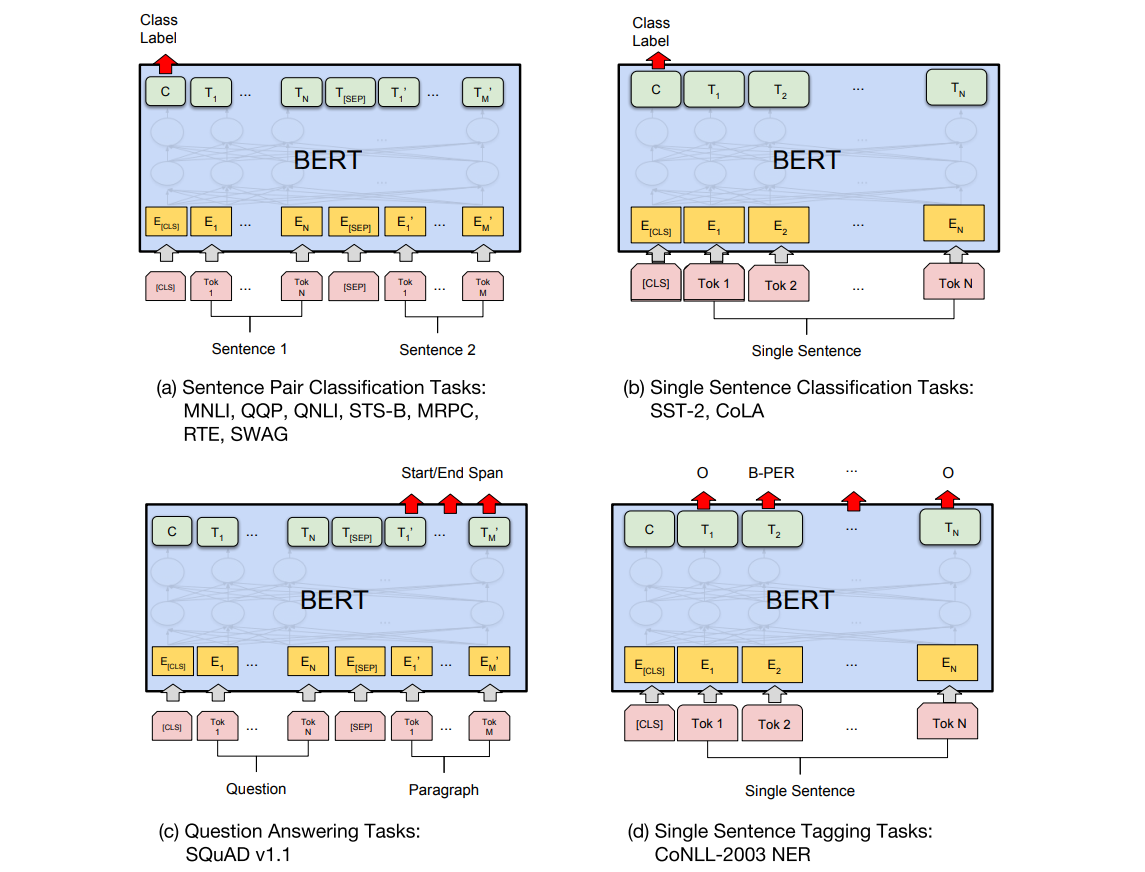
\includegraphics[width = 8.50cm]{figure/bert-finetune.png}\\ 
	\citebutton{Source: Devlin et al., 2019}{https://aclanthology.org/N19-1423.pdf}
	\end{figure}
\end{frame}

% ------------------------------------------------------------------------------

\begin{frame}{Fine-Tuning BERT}

\vspace{1.5cm}

	\begin{figure}
	\centering
		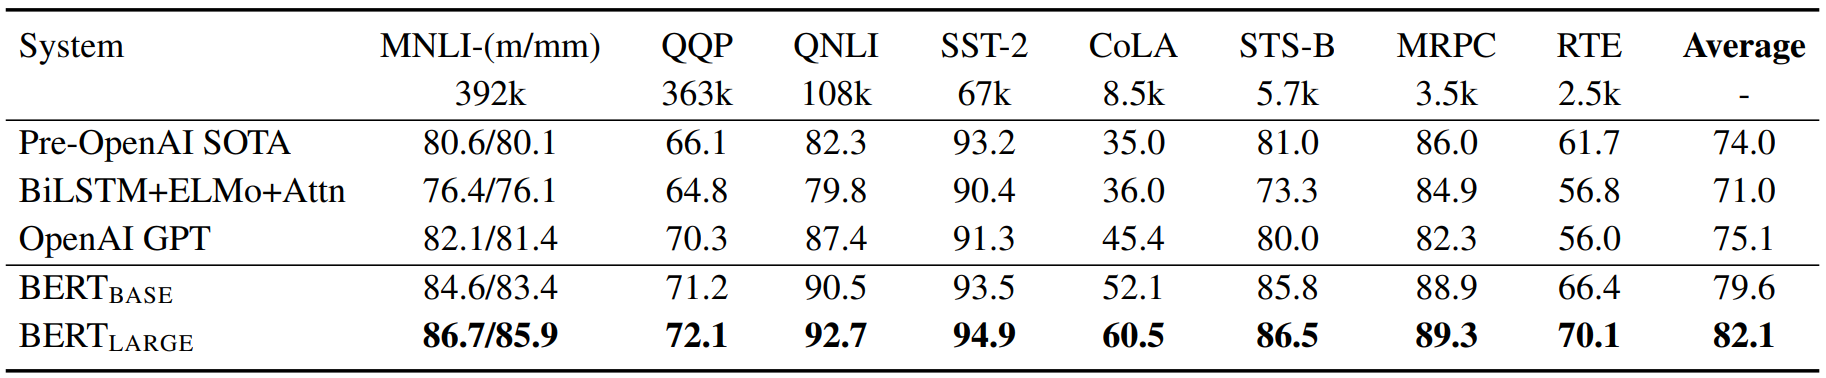
\includegraphics[width = 11cm]{figure/bert-sota.png}\\ 
	\citebutton{Source: Devlin et al., 2019}{https://aclanthology.org/N19-1423.pdf}
	\end{figure}
\begin{itemize}
	\item Performance of BERT on the GLUE Benchmark \citebutton{Wang et al., 2018}{https://gluebenchmark.com/}
	\item Beats all of the previous state-of-the-art models
	\item In the meantime: Other models (way) better than BERT
\end{itemize}

\end{frame}

% ------------------------------------------------------------------------------

\begin{frame}{Fine-tuning details}

\vfill

\begin{itemize}
	\item Relatively cheap compared to pre-training:
		\begin{itemize}
			\item $<$ 1 hour on a single Cloud TPU
			\item "a few hours" on a GPU
		\end{itemize}
	\item Recommendations for hyperparameters:
		\begin{itemize}
			\item \textbf{Batch Size:} 16, 32
			\item \textbf{Adam learning rate:} 5e-5, 3e-5, 2e-5
			\item \textbf{\#epochs:} 2, 3, 4
			\item \textbf{Dropout probability:} 0.1
		\end{itemize}
	\item Data sets w/ > 100k labeled examples rather insensitive to hyperparameters
\end{itemize}
	
\vfill

\end{frame}

% ------------------------------------------------------------------------------

\begin{frame}{Feature Extraction from BERT}

\vfill

	\begin{figure}
		\centering
		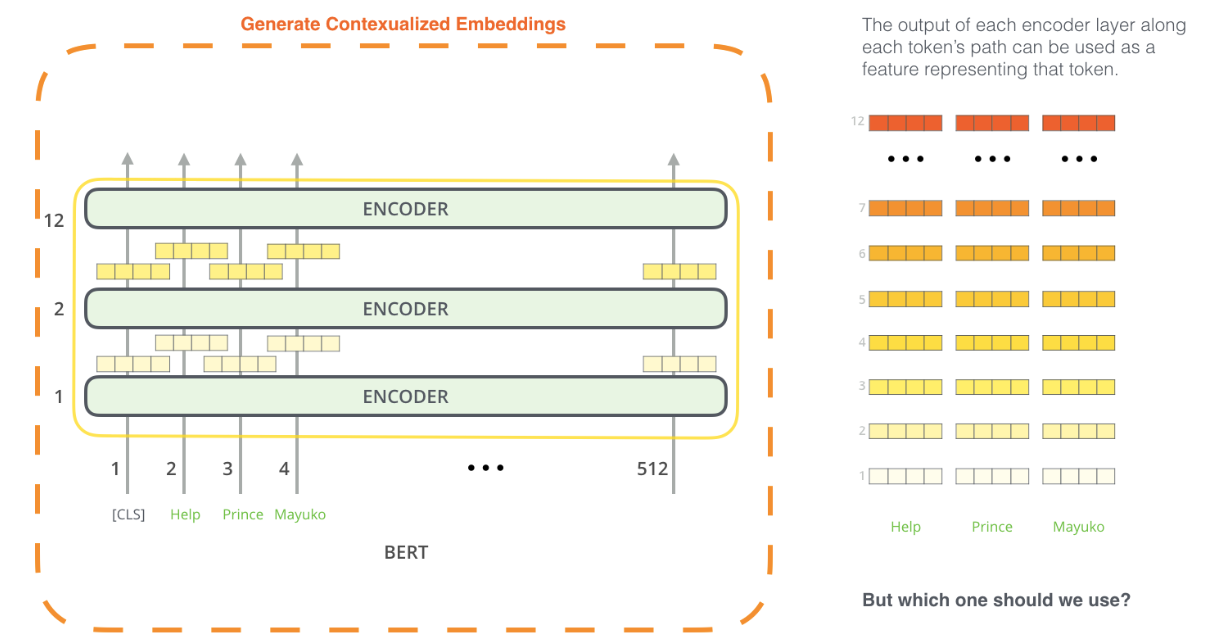
\includegraphics[width = 11cm]{figure/bert-featextr.png}\\ 
		\citebutton{Source: Jay Alammar}{https://jalammar.github.io/illustrated-bert/}
	\end{figure}

\vfill

\end{frame}

% ------------------------------------------------------------------------------

\begin{frame}{Feature Extraction from BERT}

	\begin{figure}
	\centering
		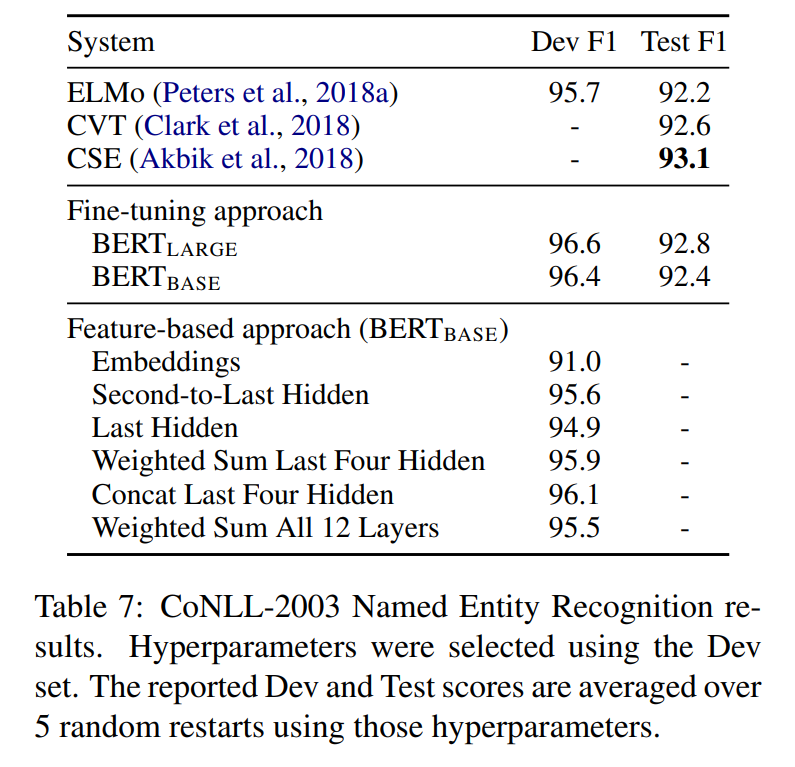
\includegraphics[width = 6.38cm]{figure/bert-featextr-results.png}\\ 
	\citebutton{Source: Devlin et al., 2019}{https://aclanthology.org/N19-1423.pdf}
	\end{figure}

\end{frame}

%%%%%%%%%%%%%%%%%%%%%%%%%%%%%%%%%%%%%%%%%%%%%%%%%%%%%%%%%%%%%%%%%%%%
\section{T5: Everything Is Text-to-Text}
%%%%%%%%%%%%%%%%%%%%%%%%%%%%%%%%%%%%%%%%%%%%%%%%%%%%%%%%%%%%%%%%%%%%
% Source: DL4NLP chapter06-post-bert-t5/slides-63-t5.tex

\begin{frame}{Revisiting text-to-text tasks}

\vfill
	
	\begin{figure}
		\centering
		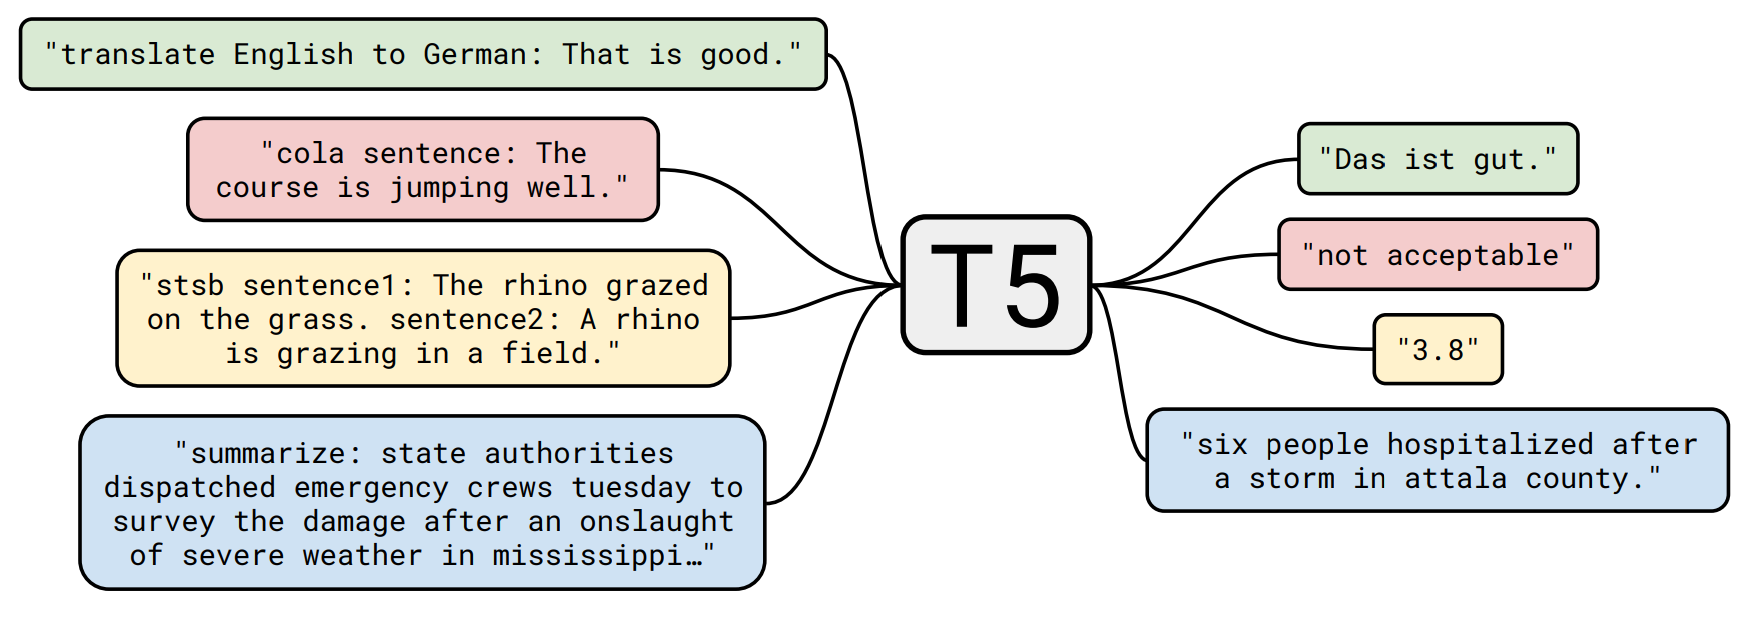
\includegraphics[width = 11cm]{figure/62-t5.png}\\ 
		\citebutton{Source: Raffel et al., 2020}{https://jmlr.org/papers/v21/20-074.html}
	\end{figure}
	
\textbf{Ingredients:}
	
\begin{itemize}
	\item \texttt{<task prefix>} for each task
	\item[] $\to$ Concatenation with the input
	\item Output label / score formatted as string
\end{itemize}
	
\vfill

\end{frame}

% ------------------------------------------------------------------------------

\begin{frame}{Text-to-Text Transfer Transformer}

\vfill

	\textbf{Short summary:}

	\begin{itemize}
		\item In short: T5 (bc of the five Ts)
		\item A complete encoder-decoder Transformer architecture
		\item[] \ques Why is this important?
		\item Relative positional embeddings
		\item All tasks reformulated as text-to-text tasks
		\item[] $\to$ Probably the most important innovation of this work
		\item From BERT-size $\times2$ (since enc-dec) up to 11B parameters
		\item Paradigm shift from \textit{Sequential Transfer Learning} towards true \textit{Multi-Task Learning}
	\end{itemize}
	
	\vspace{.5cm}

	\begin{center}
		\href{https://1.bp.blogspot.com/-o4oiOExxq1s/Xk26XPC3haI/AAAAAAAAFU8/NBlvOWB84L0PTYy9TzZBaLf6fwPGJTR0QCLcBGAsYHQ/s1600/image3.gif}{\textbf{\beamergotobutton{Nice Animation (similar to figure before)}}}
	\end{center}
	
\vfill

\end{frame}

% ------------------------------------------------------------------------------

\begin{frame}{input and output format}

\vfill

	\textbf{Input Side:}

	\begin{itemize}
		\item SentencePiece framework w/ WordPiece tokens
		\item Add task-specific (text) prefix to the original input
		\item Choice of the prefix: Hyperparameter!! 
		\item[$\to$] Changing this had limited impact
		\item[$\to$] No extensive experiments performed by the authors
	\end{itemize}
	
	\vspace{.5cm}

	\textbf{Output Side:}

	\begin{itemize}
		\item Output as a word or a piece of text (also numerical similarity scores)
		\item If output not present in set of potential alternatives, prediction considered as wrong (many other possible ways; this is not trivial)
	\end{itemize}
	
\vfill

\end{frame}

% ------------------------------------------------------------------------------

\begin{frame}{task prefix vs. prompting}

\vfill

	\textbf{Adding task-specific (text) prefix:}

	\begin{itemize}
		\item Add task-specific (text) prefix to the original input
		\item Model is fine-tuned on samples prepended with this prefix
		\item[$\to$] It learns to recognize what it is expected to do when encountering a specific prefix at test time
		\item[$\to$] Probably because of this: limited impact found by the authors
	\end{itemize}
	
	\vspace{.5cm}

	\textbf{Prompting:}

	\begin{itemize}
		\item Refers to just querying a trained w/o fine-tuning it
		\item Paradigm of Few-/Zero-Shot Learning
		\item This is found to have a \textit{huge} impact on model performance
	\end{itemize}
	
\vfill

\end{frame}

% ------------------------------------------------------------------------------

\begin{frame}{architectural differences}

\vfill
	
	\textbf{Attention patterns (top) and Schematics of considered architectures (bottom)}
	
	\begin{figure}
		\centering
		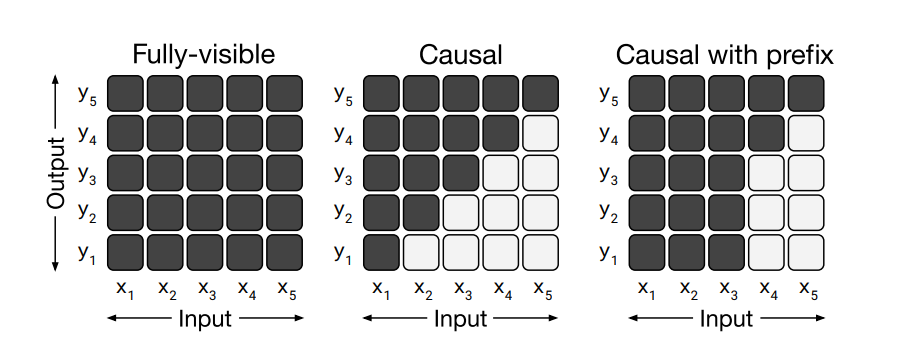
\includegraphics[width = 6.38cm]{figure/63-mask-patterns.png}\\ 
		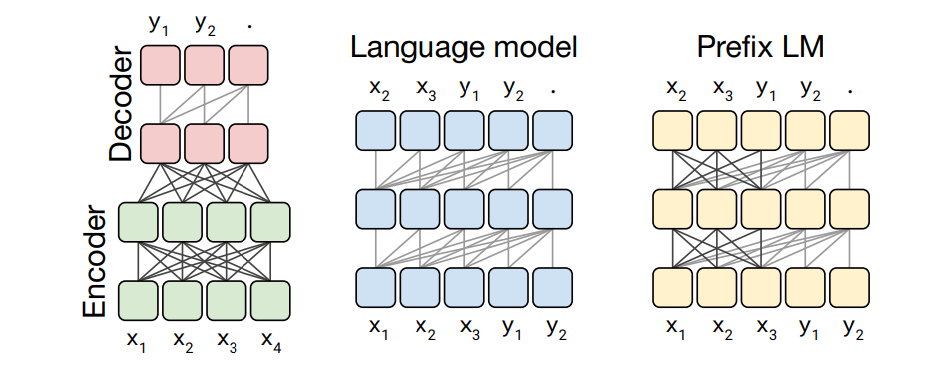
\includegraphics[width = 6.38cm]{figure/63-schematics.png}\\ 
		\citebutton{Source: Raffel et al., 2020}{https://jmlr.org/papers/v21/20-074.html}
	\end{figure}
	
\vfill

\end{frame}

% ------------------------------------------------------------------------------

\begin{frame}{pre-training objective}

\vfill
	
	\begin{figure}
		\centering
		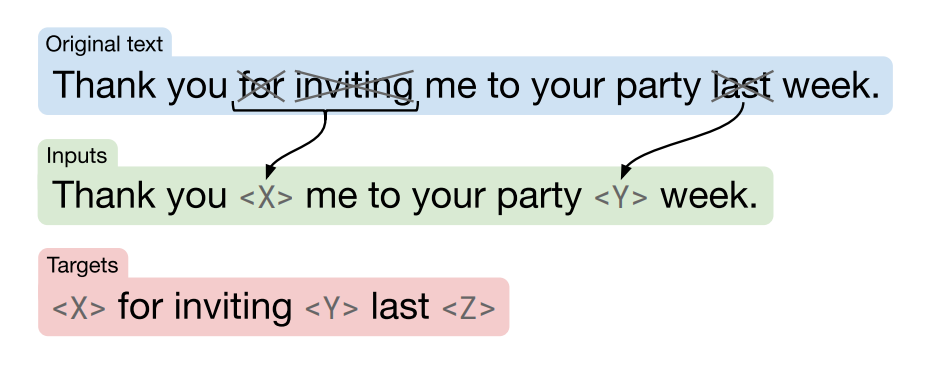
\includegraphics[width = 11cm]{figure/63-t5-span-pred.png}\\ 
		\citebutton{Source: Raffel et al., 2020}{https://jmlr.org/papers/v21/20-074.html}
	\end{figure}
	
	\begin{enumerate}
		\item Mark spans in input sequence for corruptions
		\item Replace tokens with sentinel tokens
		\item Predict sentinel tokens and replaced tokens
	\end{enumerate}
	
\vfill

\end{frame}

% ------------------------------------------------------------------------------

\begin{frame}{Pre-training objectives}

\vfill

	\begin{itemize}
		\item Authors experimented with different objectives
		\item Most of them rely in some way on MLM
	\end{itemize}
	
	\begin{figure}
		\centering
		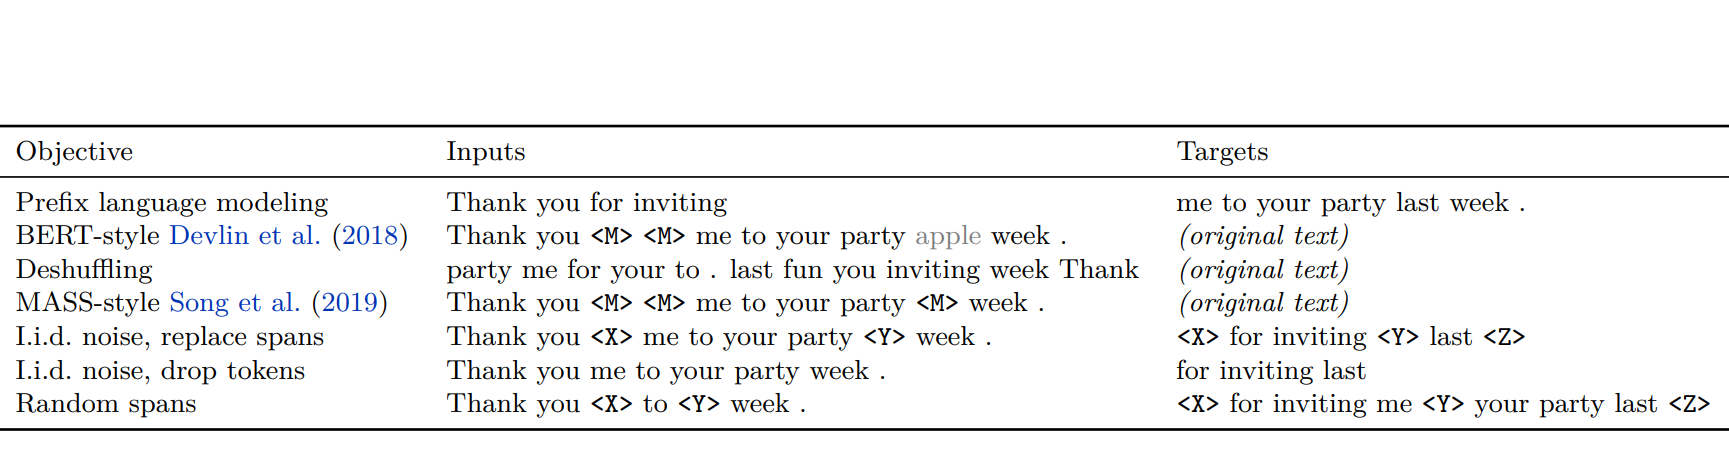
\includegraphics[width = 11cm]{figure/63-t5-objectives1.png}\\ 
		\citebutton{Source: Raffel et al., 2020}{https://jmlr.org/papers/v21/20-074.html}
	\end{figure}
	
\vfill

\end{frame}

% ------------------------------------------------------------------------------

\begin{frame}{Pre-training objectives}

\vfill

	\begin{figure}
		\centering
		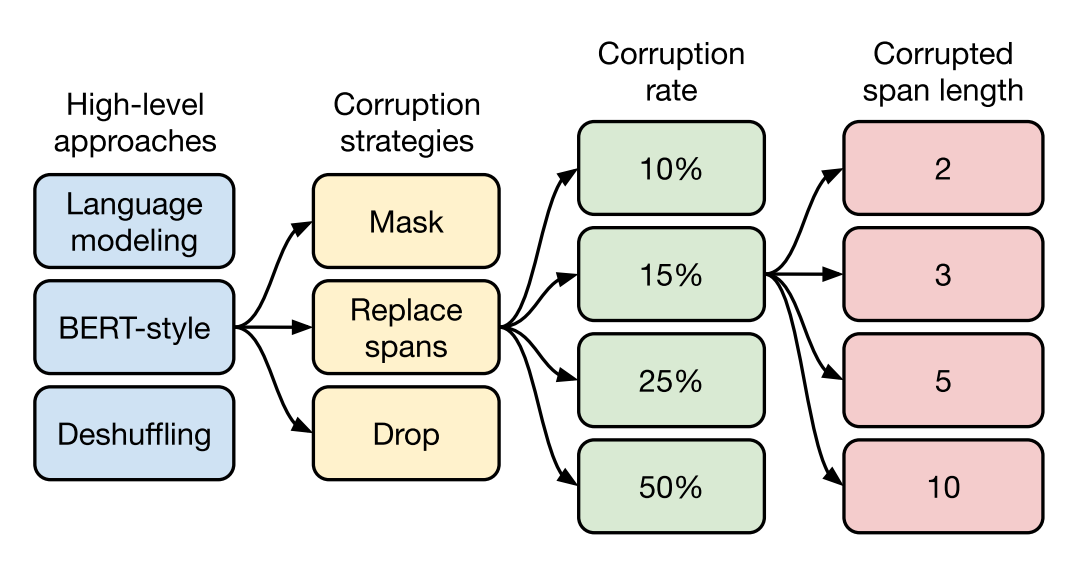
\includegraphics[width = 11cm]{figure/63-t5-objectives2.png}\\ 
		\citebutton{Source: Raffel et al., 2020}{https://jmlr.org/papers/v21/20-074.html}
	\end{figure}
	
\vfill

\end{frame}

% ------------------------------------------------------------------------------

\begin{frame}{The \textbf{C}olossal \textbf{C}lean \textbf{C}rawled \textbf{C}orpus (C4)}

\vfill

	\begin{itemize}
		\item Effort to measure the effect of quality, characteristics \& size of the pre-training resources
		\item Common Crawl as basis, careful cleaning and filtering for English language
		\item Orders of magnitude larger (750GB) compared to commonly used corpora 
	\end{itemize}
	
\vfill

\end{frame}

% ------------------------------------------------------------------------------

\begin{frame}{The \textbf{C}olossal \textbf{C}lean \textbf{C}rawled \textbf{C}orpus (C4)}

\vfill
	
	\textbf{Experiments (with respect to C4)}
	
	\begin{figure}
		\centering
		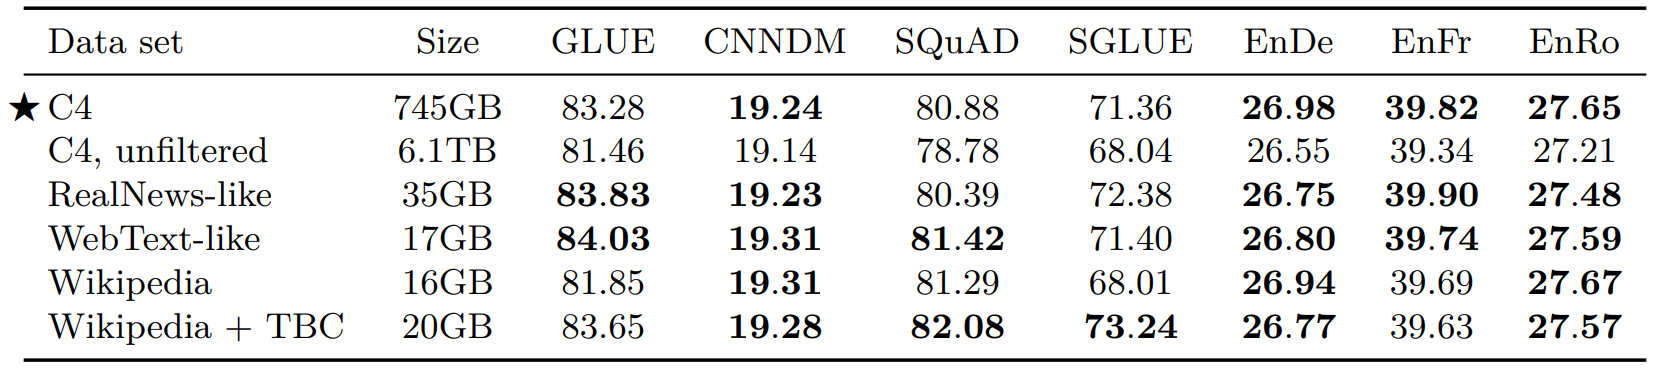
\includegraphics[width = 9cm]{figure/63-c4-characteristics.png}\\ 
		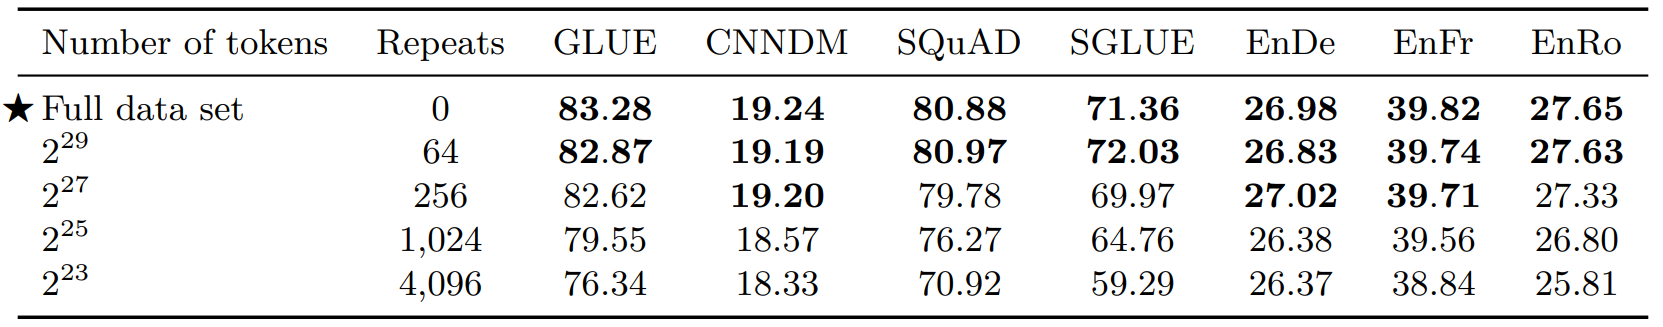
\includegraphics[width = 9cm]{figure/63-c4-size.png}\\ 
		\citebutton{Source: Raffel et al., 2020}{https://jmlr.org/papers/v21/20-074.html}
	\end{figure}
	
\vfill

\end{frame}

% ------------------------------------------------------------------------------

\begin{frame}{T5 - Exhaustive Experiments}

\vfill

	\textbf{Performed experiments with respect to ..}
	
	\begin{itemize}
		\item \textit{.. architecture, size \& objective}
		\item[$\to$] enc, dec, enc-dec
		\item[$\to$] Between 60M and 11B parameters
		\item \textit{.. details of the Denoising objective (which was found to work best)}
		\item \textit{.. fine-tuning methods}
		\item[$\to$] Adapter layers
		\item[$\to$] Gradual Unfreezing
		\item \textit{.. Multi-task learning strategies}
		\item[$\to$] Examples-proportional mixing
		\item[$\to$] Temperature-scaled mixing
	\end{itemize}
	
\vfill

\end{frame}

% ------------------------------------------------------------------------------

\begin{frame}{Different T5 versions}
\textit{Similar to BERT T5 has different versions, which all have a different parameter count} \citebutton{Raffel et al., 2020}{https://arxiv.org/abs/1910.10683}

\begin{table}[h!]
\centering
\small % Reduce font size
\begin{tabular}{|c|c|c|c|c|c|c|}
\hline
\textbf{Model} & \textbf{Parameters} & $\bm{n_{layers}}$ & $\bm{d_{model}}$ & $\bm{d_{FFN}}$ & $\bm{d_{qkv}}$ & $\bm{n_{heads}}$ \\ \hline
small  & 60M  & 6  & 512  & 2048 & 64 & 8 \\ \hline
base   & 220M & 12 & 768  & 3072 & 64 & 12 \\ \hline
large  & 770M & 24 & 1024 & 4096 & 64 & 16 \\ \hline
3B     & 3B   & 24 & 1024 & 16384 & 128 & 32 \\ \hline
11B    & 11B  & 24 & 1024 & 65536 & 128 & 128 \\ \hline
\end{tabular}
\end{table}

\begin{itemize}
    \item For T5 small, base and large we have the following parameter count per encoder/decoder layer:
    \begin{itemize}
        \item $N_{Encoder} = 12\cdot d_{model}^2$
        \item $N_{Decoder} = 16\cdot d_{model}^2$
    \end{itemize}
		\item \textit{For T5 3B and 11B $N_{Encoder}$ and $N_{Decoder}$ are different!}
\end{itemize}
    
\end{frame}

%%%%%%%%%%%%%%%%%%%%%%%%%%%%%%%%%%%%%%%%%%%%%%%%%%%%%%%%%%%%%%%%%%%%
\section{Fine-Tuning, Prompting, Instruction Tuning}
%%%%%%%%%%%%%%%%%%%%%%%%%%%%%%%%%%%%%%%%%%%%%%%%%%%%%%%%%%%%%%%%%%%%
% Source: DL4NLP chapter09-llm/slides-91-instruction-tuning.tex

\begin{frame}{How to solve a task with language models? (1)}

\vfill

\begin{itemize}
    \item ``old-style'' single-task fine-tuning 
        \begin{itemize}
            \item supervised training
of the pretrained model
on a task-specific
        training set of size $k$ (where $k$ is not small,
        e.g., $k=100$)
        \end{itemize}
\end{itemize}

\vfill

\end{frame}

% ------------------------------------------------------------------------------

\begin{frame}{BERT finetuning example 1}

\vfill
	
	\begin{figure}
		\centering
		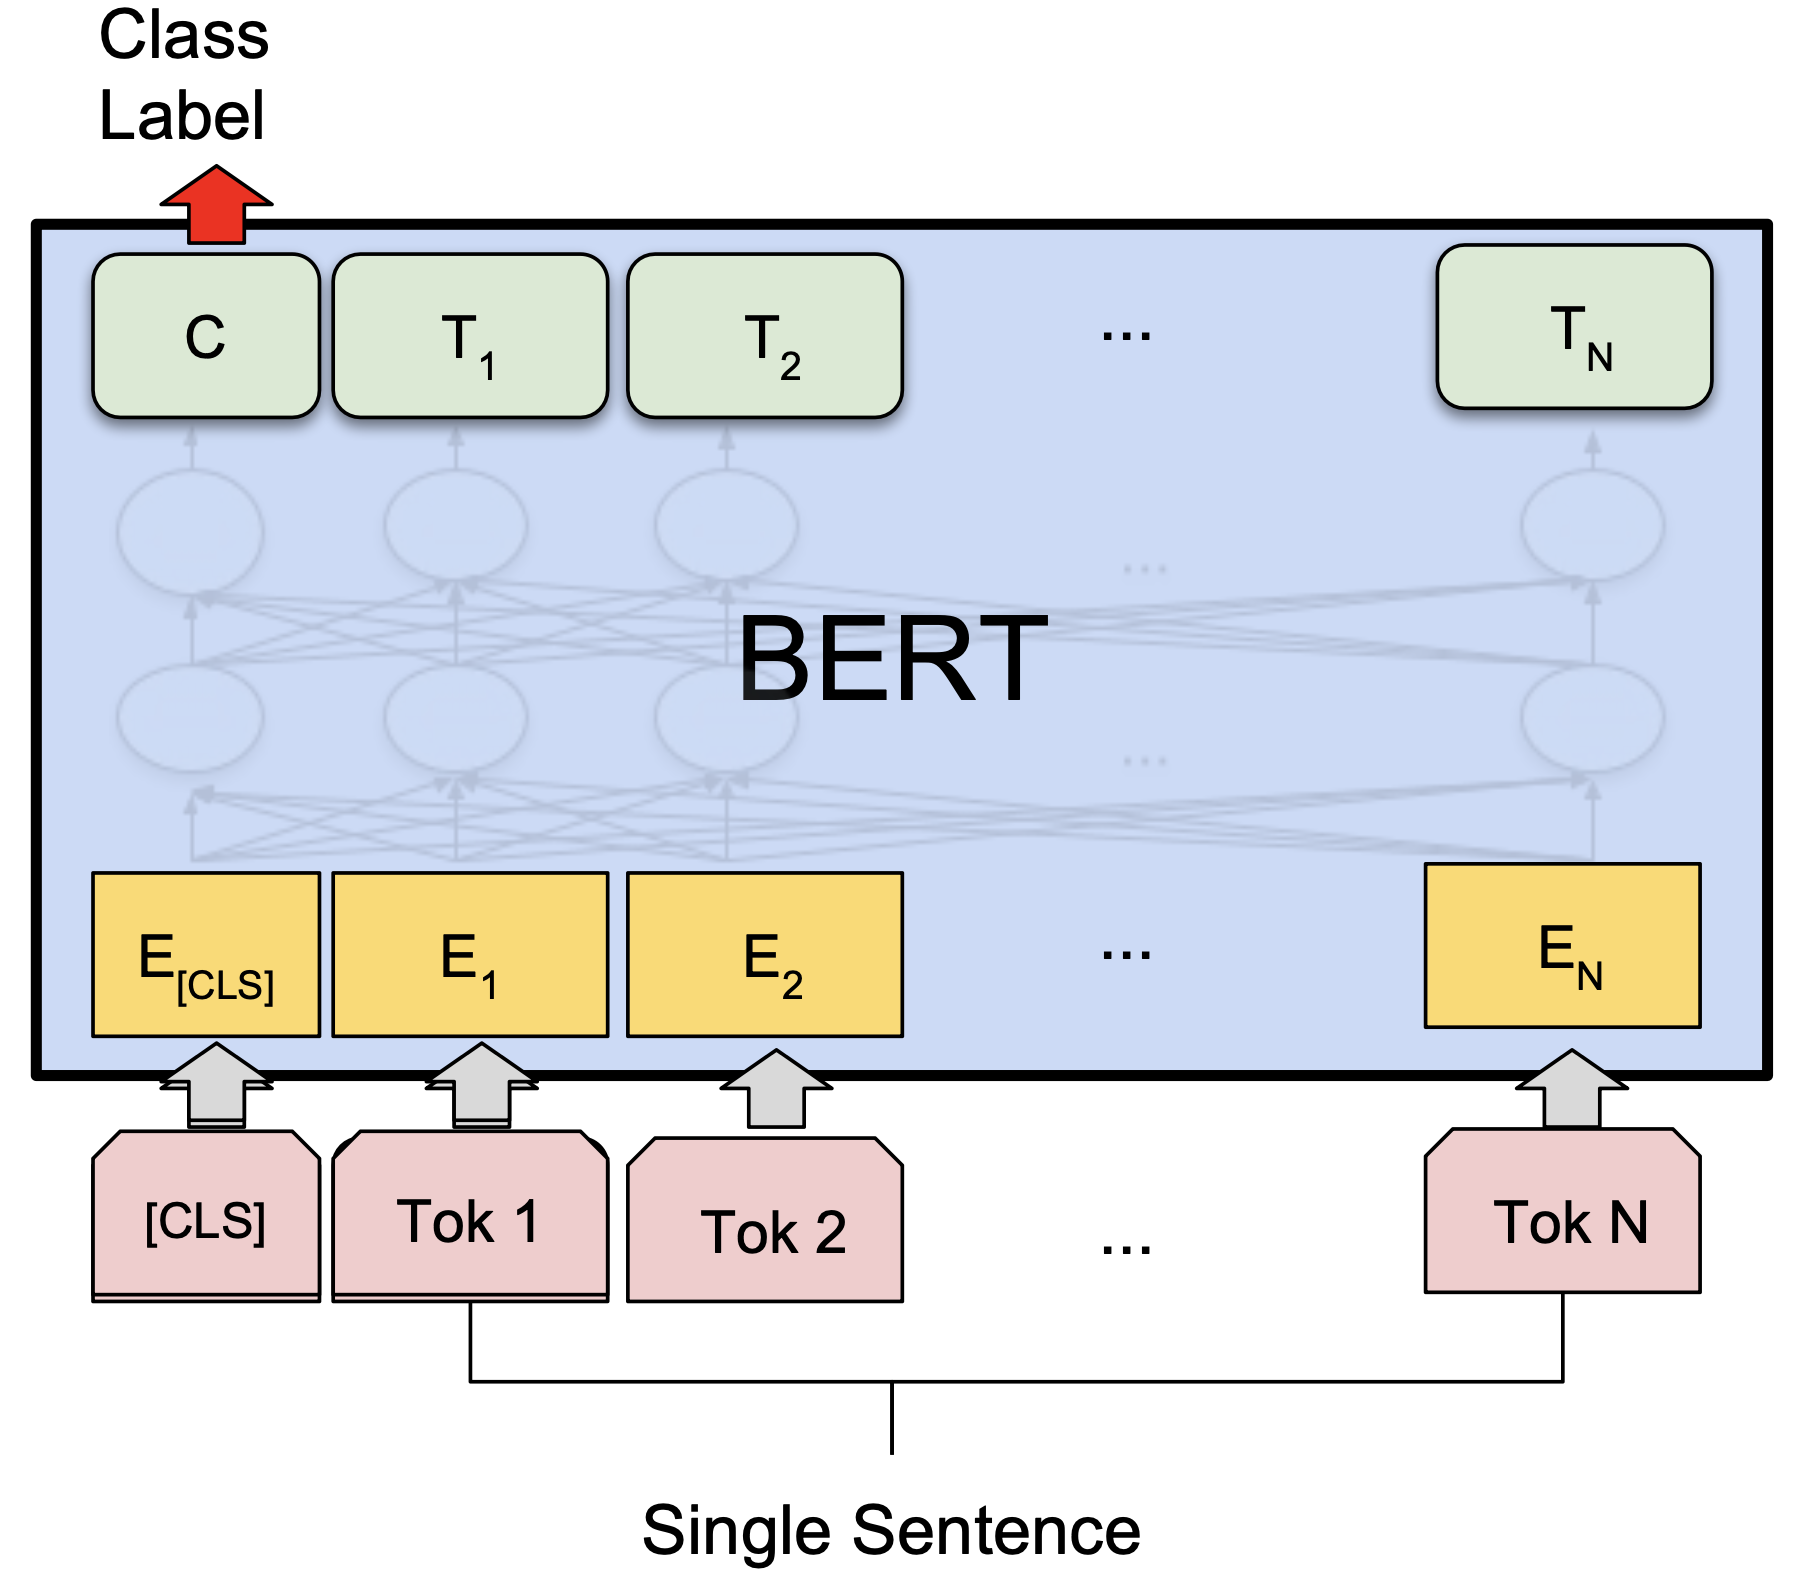
\includegraphics[height = 6cm]{figure/bertfinetune1} 
	\end{figure}

\vfill

\end{frame}

% ------------------------------------------------------------------------------

\begin{frame}{BERT finetuning example 2}

\vfill
	
	\begin{figure}
		\centering
		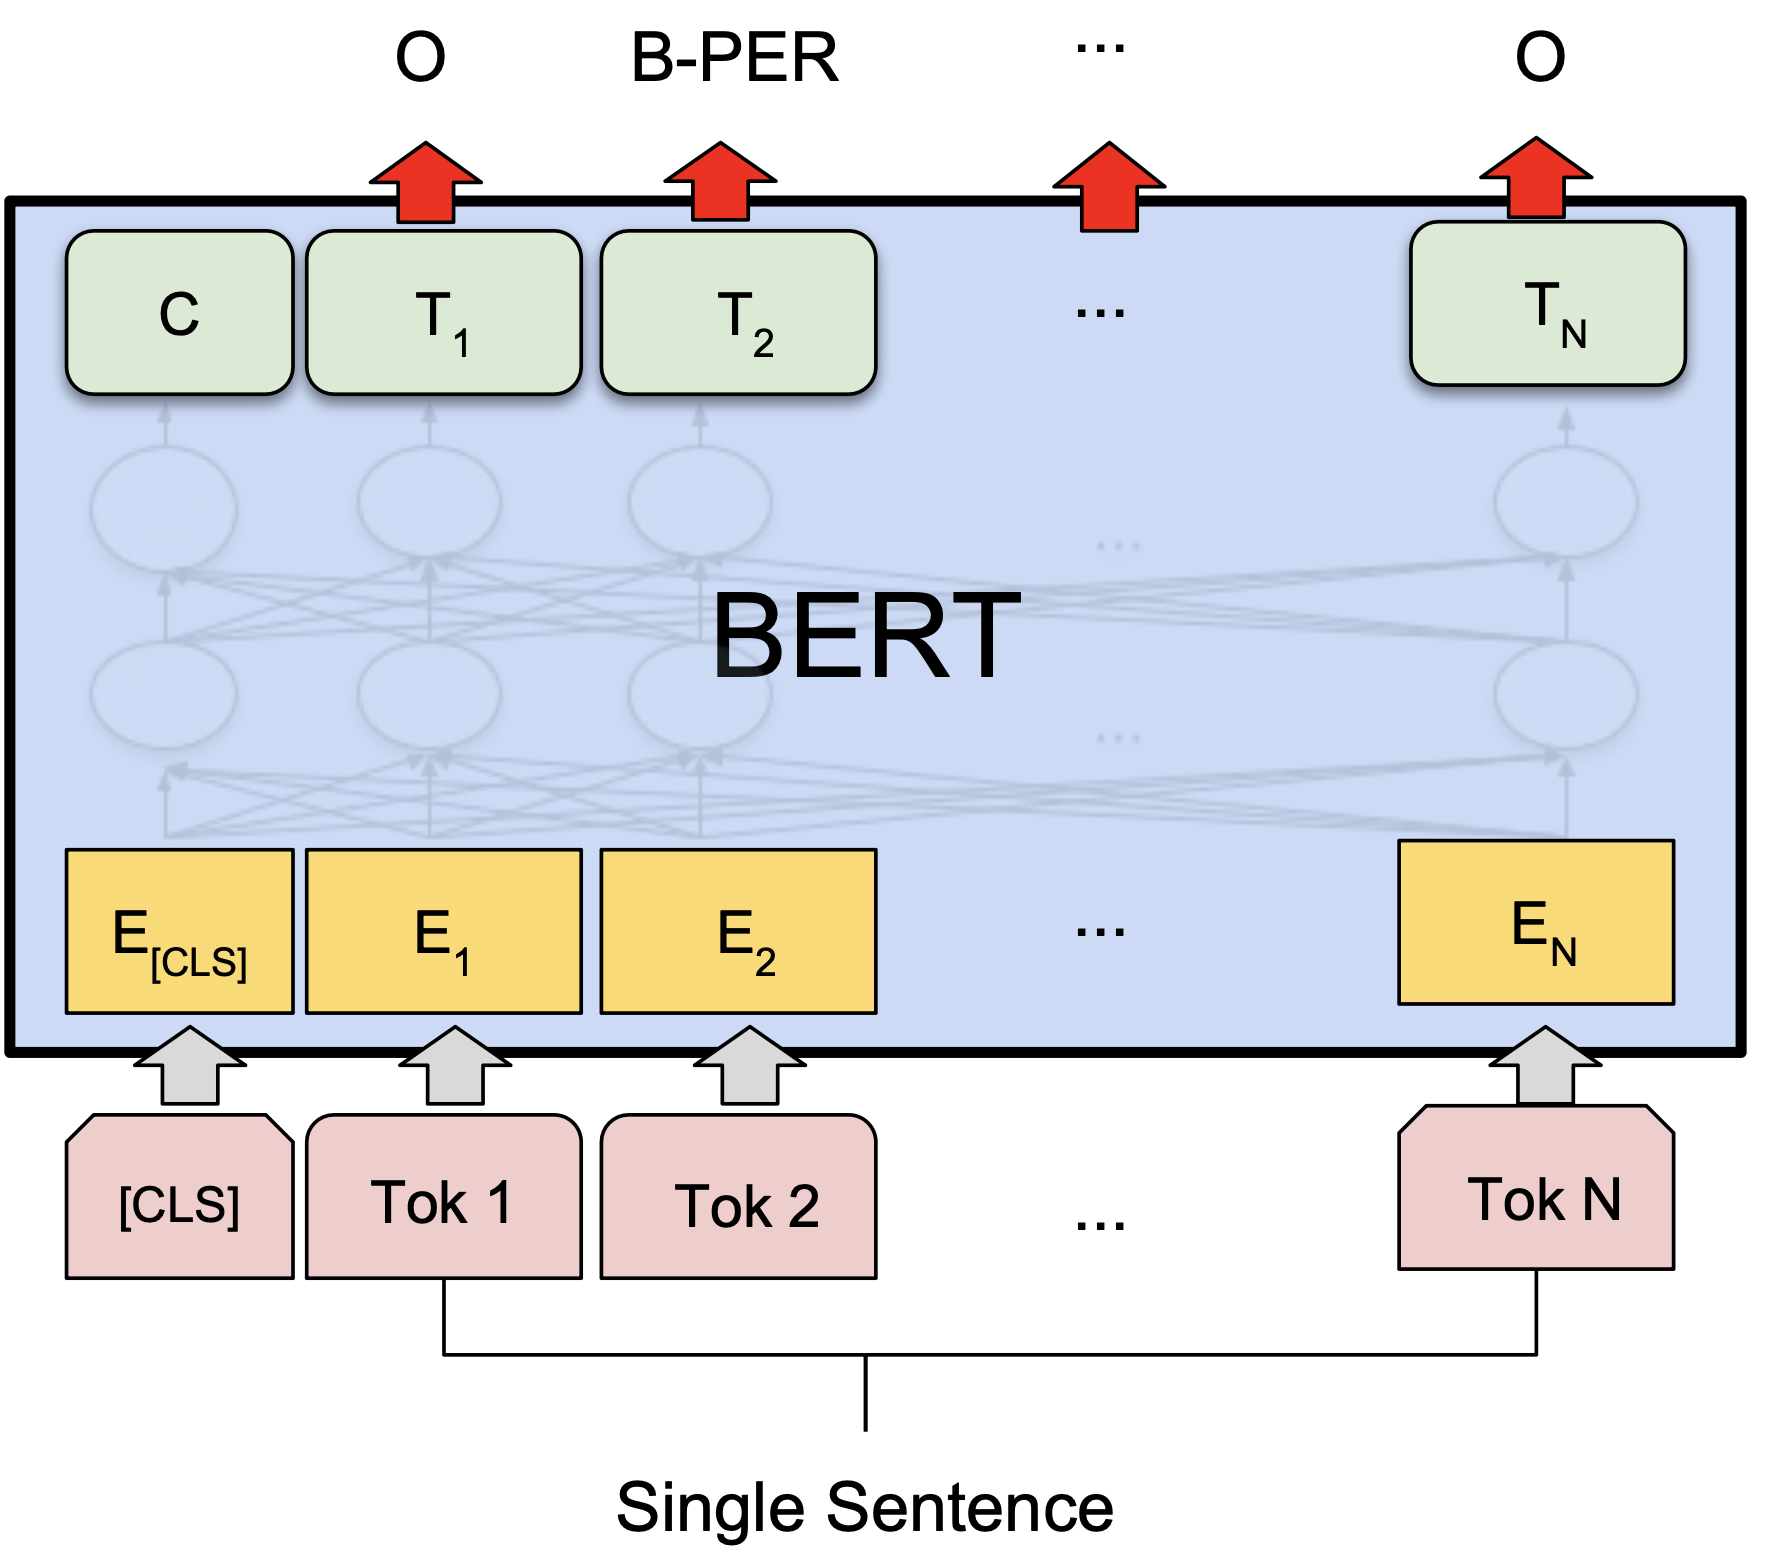
\includegraphics[height = 6cm]{figure/bertfinetune2} 
	\end{figure}

\vfill

\end{frame}

% ------------------------------------------------------------------------------

\begin{frame}{How to solve a task with language models? (1)}

\vfill

\begin{itemize}
    \item ``old-style'' single-task fine-tuning 
        \begin{itemize}
            \item supervised training
of the pretrained model
on a task-specific
        training set of size $k$ (where $k$ is not small,
        e.g., $k=100$)
        \item the output can be an arbitrary category (e.g.,
        ``0'', ``1'' for sentiment analysis)
        \item (this is the typical way encoder models like
        BERT are used)
            \item alternatively, the output can be a
        meaningful ``verbalizer'' (e.g., ``negative'',
        ``positive'' for sentiment analysis)
        		\citebutton{Schick et al.,
        2020}{https://arxiv.org/abs/2009.07118}
        \item still very much relevant if you need to deploy
        a small efficient model for a focused task
        \end{itemize}
\end{itemize}

\vfill

\end{frame}

% ------------------------------------------------------------------------------

\begin{frame}{How to solve a task with language models? (2)}

\vfill

\begin{itemize}
    \item few-shot prompting
        \begin{itemize}
            \item provide, in-context,  $k$ (where $k$ is small, e.g., $k=5$) examples of what the model is
supposed to do
        \item the model will then often complete the task
        just based on analogy to these few shots
        \item this is a typical way of using current
        autoregressive models for tasks
\item no change to the parameters of the model, i.e., no training
\end{itemize}
\end{itemize}

\vfill

\end{frame}

% ------------------------------------------------------------------------------

\begin{frame}{few-shot prompting example}

\vfill
	
	\begin{figure}
		\centering
		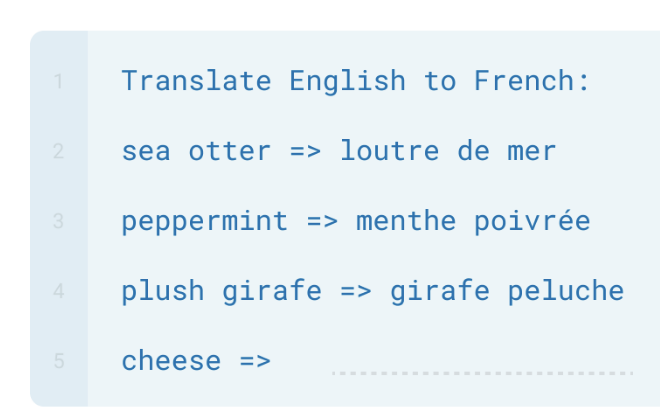
\includegraphics[height = 5.10cm]{figure/fewshotprompting} 
	\end{figure}

(from gpt3 paper -- ``Translate English to French'' should
appear four times to make it a 3-shot example that has 3
identical shots as required by the definition of few-shot prompting)

\vfill

\end{frame}

% ------------------------------------------------------------------------------

\begin{frame}{How to solve a task with language models? (3)}

\vfill

\begin{itemize}
\item multi-task finetuning
        \begin{itemize}
        \item finetuning on a large training set of *many* tasks
        \item the more tasks the better
        \item method 1: consistent task format, e.g., each
        task is reformulated into a question-answering format
        \item method 2: more open task format
\item ideally: task format includes ``instructions'',
similar to verbalizer
            \item Examples: T0, T5 and FLAN, see below
        \end{itemize}
\end{itemize}

\vfill

\end{frame}

% ------------------------------------------------------------------------------



% ------------------------------------------------------------------------------

\begin{frame}{issues with single-task fine-tuning}

\vfill

\begin{itemize}
    \item The result is a single-task model.
%\item Sequential transfer learning instead of true multi-task learning
\begin{itemize}
    \item Generalization of the model 
             is only w.r.t. to one task / data distribution
\end{itemize}
    \item Requires  annotated
        data (e.g., $k=100$)
%    \item Single-task models have poor few-shot capabilities
            \item \ques Could there be other tasks that
        might benefit?
 %           \item \ques What about related domains / languages?
\end{itemize}

\vfill

\end{frame}

% ------------------------------------------------------------------------------

\begin{frame}{issues with few-shot prompting: (1) classification}

\vfill

\begin{itemize}
    \item Assumption: Model has learned about the task during (unsupervised) pre-training 
    \item Write prompt so that  a direct response must be
    given by the language model.
\begin{itemize}
        \item Just a label, just yes/no answer, just a name
    in QA
\end{itemize}
    \item This is not natural dialogic behavior: humans
    typically don't
    just answer with a label, yes/no, a name (although
    sometimes they do)
%\item Again: Prompting works best if the task has occurred during
%unsupervised training.
\item Current use of the word ``prompt'' is more general: basically
anything you type into the LLM context window
 %   \item \ques For which tasks is this expected to work well?
% key: does the task (or as imilar task) occur in preatraing
% machine translation example:  example of what works well
% complex reasoning example: example of what does notw ork well
%    \item \textit{Lack of interpretability}
%    \begin{itemize}
%        \item Just the answer w/o explanation
%        \item Big concern about LLMs in general

%    \item \textit{Misalignment with human needs}
%    \begin{itemize}
%        \item Out of context answers
%        \item Harmful answers
%    \end{itemize}
\end{itemize}

\vfill

\end{frame}

% ------------------------------------------------------------------------------

\begin{frame}{issues with few-shot prompting:\\ (2) text generation}

\vfill

\begin{itemize}
%\item Very similar to (1) classification
    \item Again, assumption: Model has learned about the task during (unsupervised) pre-training 
    \item Again: Write prompt so that  a direct response must be
    given by the language model.
\item Works best if the task has occurred during
unsupervised training.
    \item \ques For which tasks is this expected to work well?
% summarization, translation because they occur in
% pretraining data
\end{itemize}

\vfill

\end{frame}

% ------------------------------------------------------------------------------

\begin{frame}{Multi-task learning: FLAN/T0/T5}

\vfill
	
	\begin{figure}
		\centering
		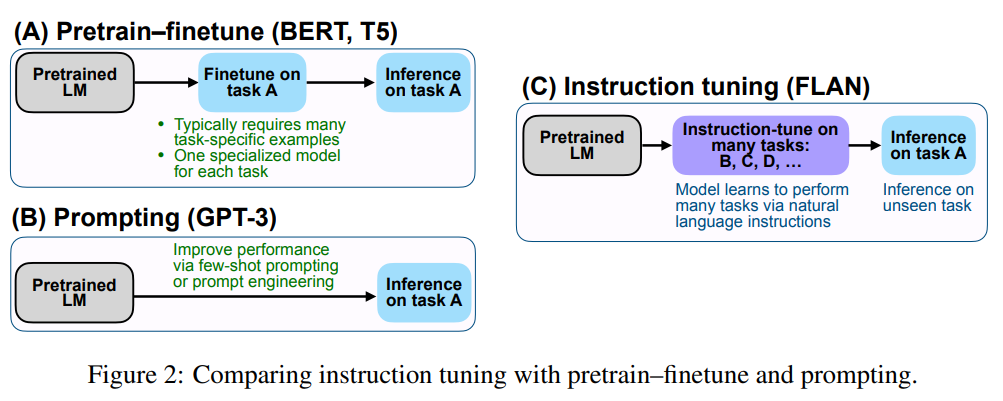
\includegraphics[width = 11cm]{figure/81-flan.png}\\ 
		\citebutton{Source: Wei et al., 2021}{https://arxiv.org/abs/2109.01652}
	\end{figure}

\vfill

\end{frame}

% ------------------------------------------------------------------------------

\begin{frame}{Multitask Prompted Training}

\vfill

\begin{itemize}
    \item Benchmark for Evaluation:
        \begin{itemize}
        \item Instead of using held-out *samples* (as is
        standard in NLP) \ldots
        \item \ldots we now use held-out *tasks*
%            \item Held-out \textit{tasks} instead of just held-out samples as a test set\\
            \item All data sets belonging to a held-out task go to the test set
            \item Generalization across tasks %/ data distributions
        \end{itemize}
    \item The ``prompts'' are key here to
facilitate
        transfer to new tasks:  the model can solve new
        tasks by generalizing from  the train prompts and the ability to generate text outputs.
\end{itemize}

\vfill

\end{frame}

% ------------------------------------------------------------------------------



% ------------------------------------------------------------------------------

\begin{frame}[allowframebreaks]{Multi-task training vs Instruction tuning}
% fit16:9: allowframebreaks instead of shrinking text


\vfill

\begin{itemize}
\item The term ``instruction tuning'' was introduced by FLAN paper,
		\citebutton{Source: Wei et al., 2021}{https://arxiv.org/abs/2109.01652}
\item However, today ``instruction tuning'' refers to a wide
variety of methods that train on instruction-output pairs,
    not just tasks
  \item
    In particular,
open-ended generation and ``alignment'' 
is now included under
    the rubric ``instruction tuning'': brainstorming,
    writing a joke, give me ten analogies for concept X,
    don't use hate language, don't take positions on
    controversial political issues etc
\item These are not classical NLP tasks.
\item Our use of terminology in this class:
\item multi-task finetuning = tasks in the classical NLP
    sense
    \item instruction-tuning: a broad approach to changing
    the behavior of a raw language model (i.e., trained on
    next-word prediction) to be ``helpful, harmless and
    honest''. This includes training on classical NLP tasks,
    but it's just one part.
\end{itemize}

\vfill

\end{frame}

% ------------------------------------------------------------------------------

\begin{frame}{Fine-Tuning Conclusions}

\vfill

\begin{itemize}
\item 
     The more training tasks the better
\item Multi-task finetuning generalizes across models
    \begin{itemize}
    \item It works well on different architectures
    \end{itemize}
\item Greatly improves usability
%and mitigates some harms
\item It is relatively compute-efficient
    \begin{itemize}
    \item Pretraining is hugely expensive, finetuning and
    instruction tuning are usually much cheaper.
    \item For PaLM 540\,B it takes 0.2\,\% of pre-training compute, but improves by 9.4\,\%
    \end{itemize}
\end{itemize}

\vfill

\end{frame}

%%%%%%%%%%%%%%%%%%%%%%%%%%%%%%%%%%%%%%%%%%%%%%%%%%%%%%%%%%%%%%%%%%%%
\section{Chain-of-Thought Prompting}
%%%%%%%%%%%%%%%%%%%%%%%%%%%%%%%%%%%%%%%%%%%%%%%%%%%%%%%%%%%%%%%%%%%%
% Source: DL4NLP chapter09-llm/slides-92-chain-of-thought.tex

\begin{frame}[shrink=8]{\cotpfullcap motivation}
% fit16:9: shrink instead of allowframebreaks (the break left a near-empty second page; the two-line title costs the room)


\vfill

How to boost the reasoning capabilities of LMs? \citebutton{Wei et al., 2021}{https://arxiv.org/abs/2109.01652}

\begin{itemize}
\item Use formal approaches, e.g., logic, symbolic reasoning
    \begin{itemize}
    \item Example: \citebutton{BeliefBank}{https://arxiv.org/abs/2109.14723}
\item Difficult to train and deploy, not widely used
    \end{itemize}
\item Standard few-shot learning via prompting works for many tasks
    \begin{itemize}
    \item Still, it works poorly for many tasks that require reasoning
    \end{itemize}
\item \cotp
    \begin{itemize}
    \item A form of few-shot prompting
    \item Each ``training example'' has the form:\\ <input, \textit{chain of thought}, output>
    \item chain of thought:\\ series of reasoning steps that
    lead to the final answer
  \item application:
    reasoning tasks:
    complex, commonsense, symbolic etc
    \end{itemize}

\end{itemize}

\vfill

\end{frame}

% ------------------------------------------------------------------------------

\begin{frame}{\cotpfullcap paradigm}

\vfill

%\textbf{\cotp enables LLMs to tackle complex arithmetic, commonsense and symbolic reasoning tasks.}

\begin{figure}
    \centering
    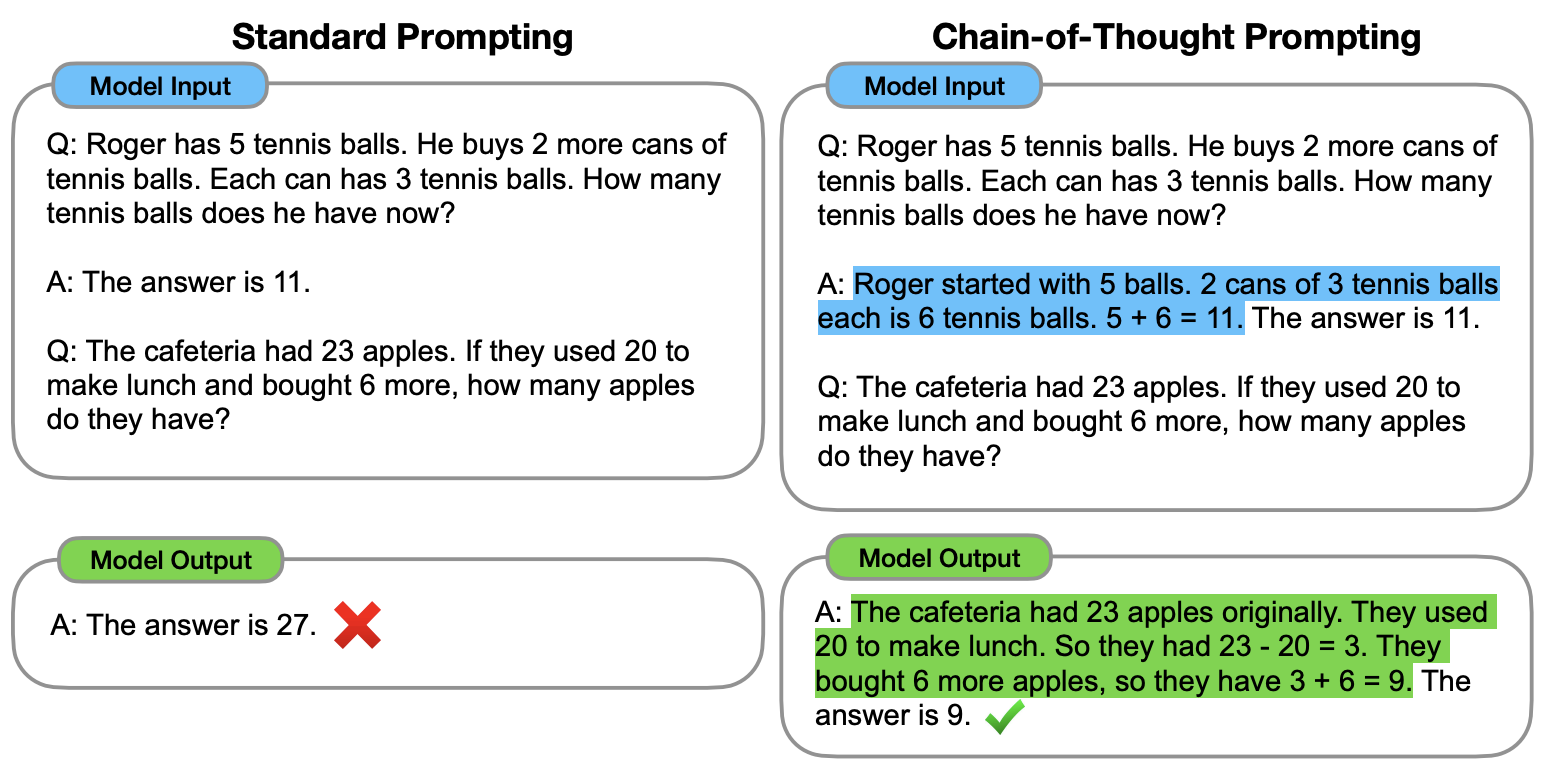
\includegraphics{figure/chain_of_thought.png}\\
    \citebutton{Source: Wei et al., 2022}{https://arxiv.org/pdf/2201.11903.pdf}
\end{figure}

\vfill

\end{frame}

% ------------------------------------------------------------------------------

\begin{frame}{\cotpfull paradigm}

\begin{figure}
    \centering
    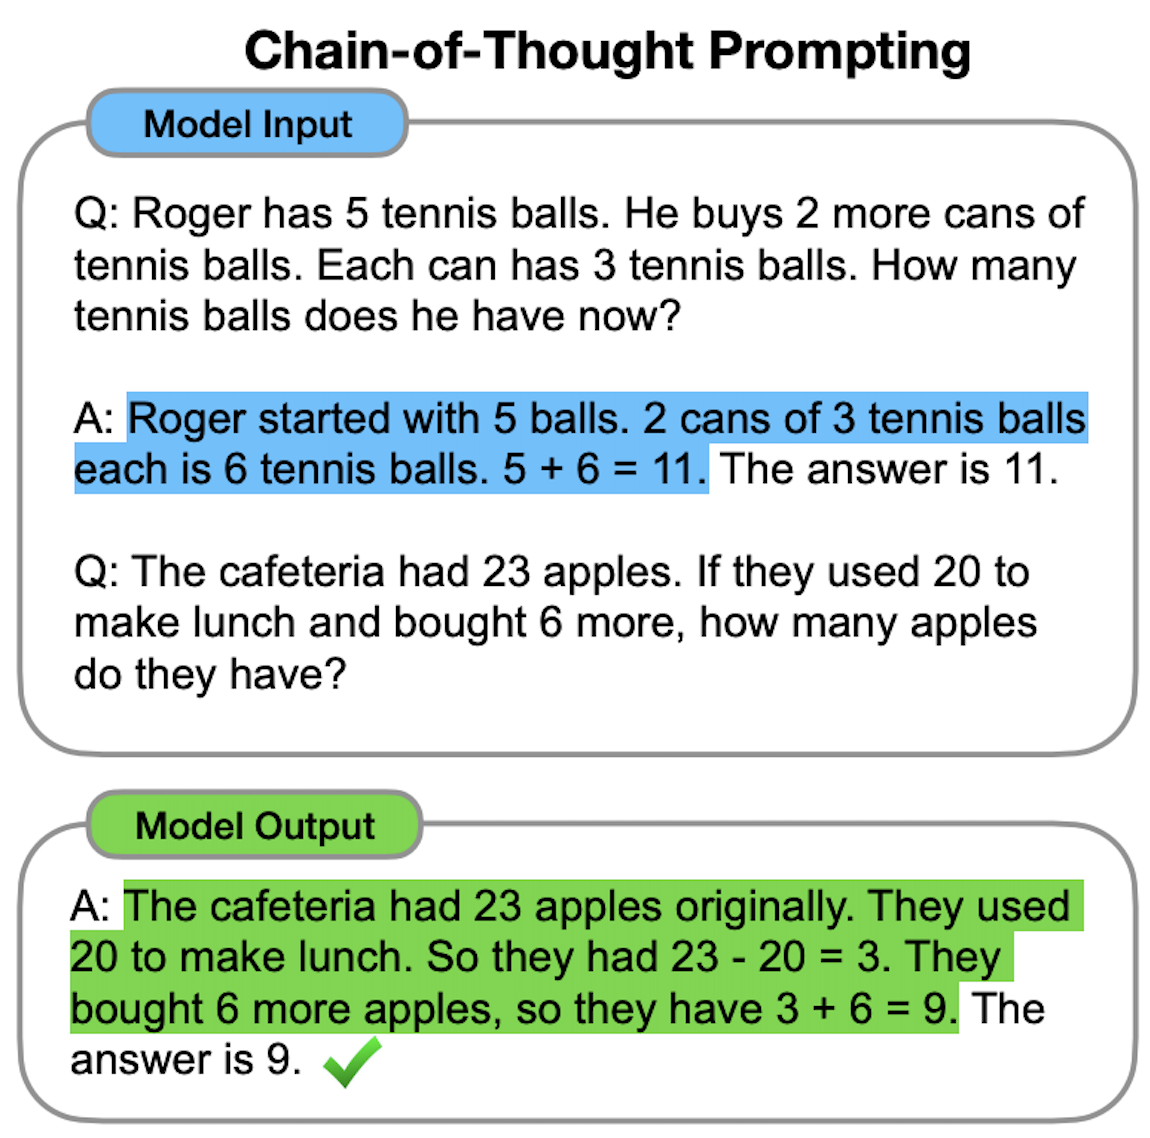
\includegraphics[height=5.95cm]{figure/chain_of_thought2.png}
\end{figure}

\end{frame}

% ------------------------------------------------------------------------------

\begin{frame}{Benefits of \cotpfull}

\vfill

\begin{itemize}
    \item Decompose multi-step problems and thus allocate more compute to problems requiring more reasoning steps.
    \item This helps LMs 
    solve problems they otherwise would not be able to solve.
    \item By describing the reasoning, interpretability is increased. It provides the possibility to observe where reasoning went wrong
    \item \cotp  is closer to how humans solve tasks using language
\end{itemize}

\vfill

\end{frame}

% ------------------------------------------------------------------------------

\begin{frame}{\cotpfull}

\vfill

\textbf{Following slides: Examples of $<$input, chain of thought, output$>$ triples for  commonsense and symbolic reasoning}

    \citebutton{Source: Wei et al., 2022}{https://arxiv.org/pdf/2201.11903.pdf}

The few shots (training examples) are omitted from these
examples to save space, but this is
\cotpfull,
 that is, the model is prompted with examples of
chain of thought reasoning.


\vfill

\end{frame}

% ------------------------------------------------------------------------------

\begin{frame}{Examples}

\vfill

\begin{figure}
    \centering
    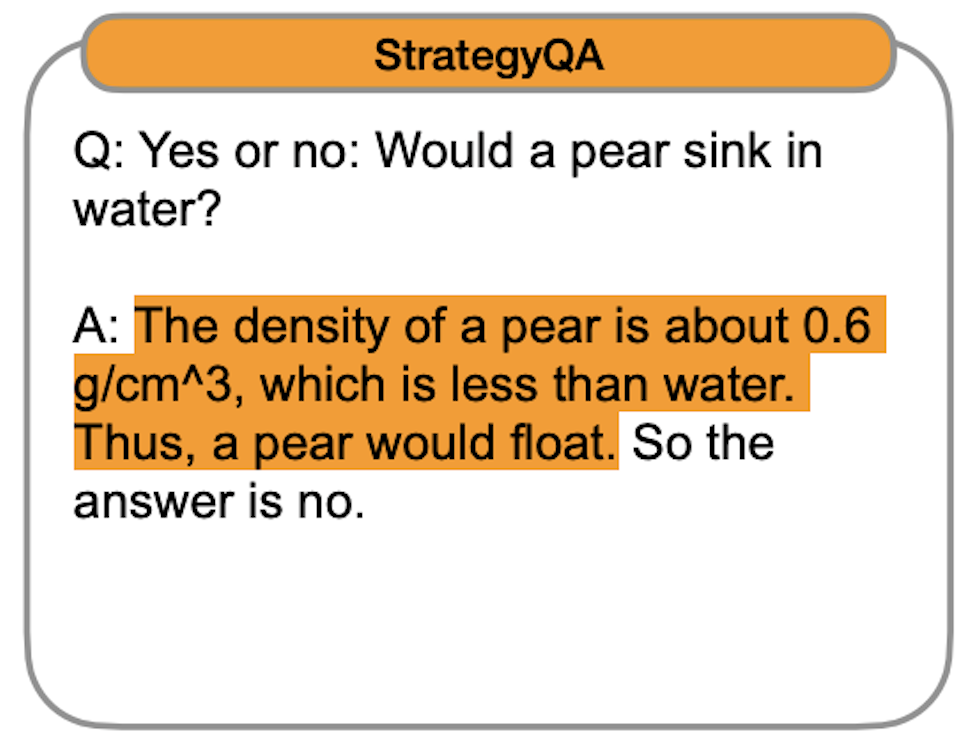
\includegraphics[height=5.95cm]{figure/cotex1.png}
\end{figure}

\vfill

\end{frame}

% ------------------------------------------------------------------------------

\begin{frame}{Examples}

\vfill

\begin{figure}
    \centering
    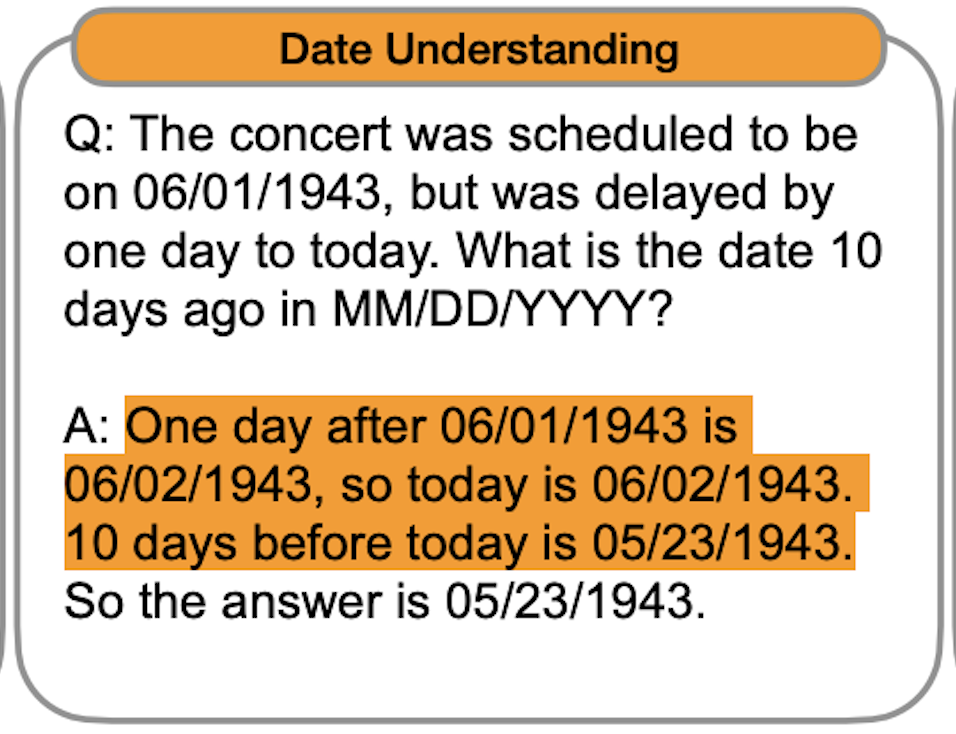
\includegraphics[height=5.95cm]{figure/cotex2.png}
\end{figure}

\vfill

\end{frame}

% ------------------------------------------------------------------------------

\begin{frame}{\cotp improves arithmetic}

\vfill
	
	\begin{figure}
		\centering
		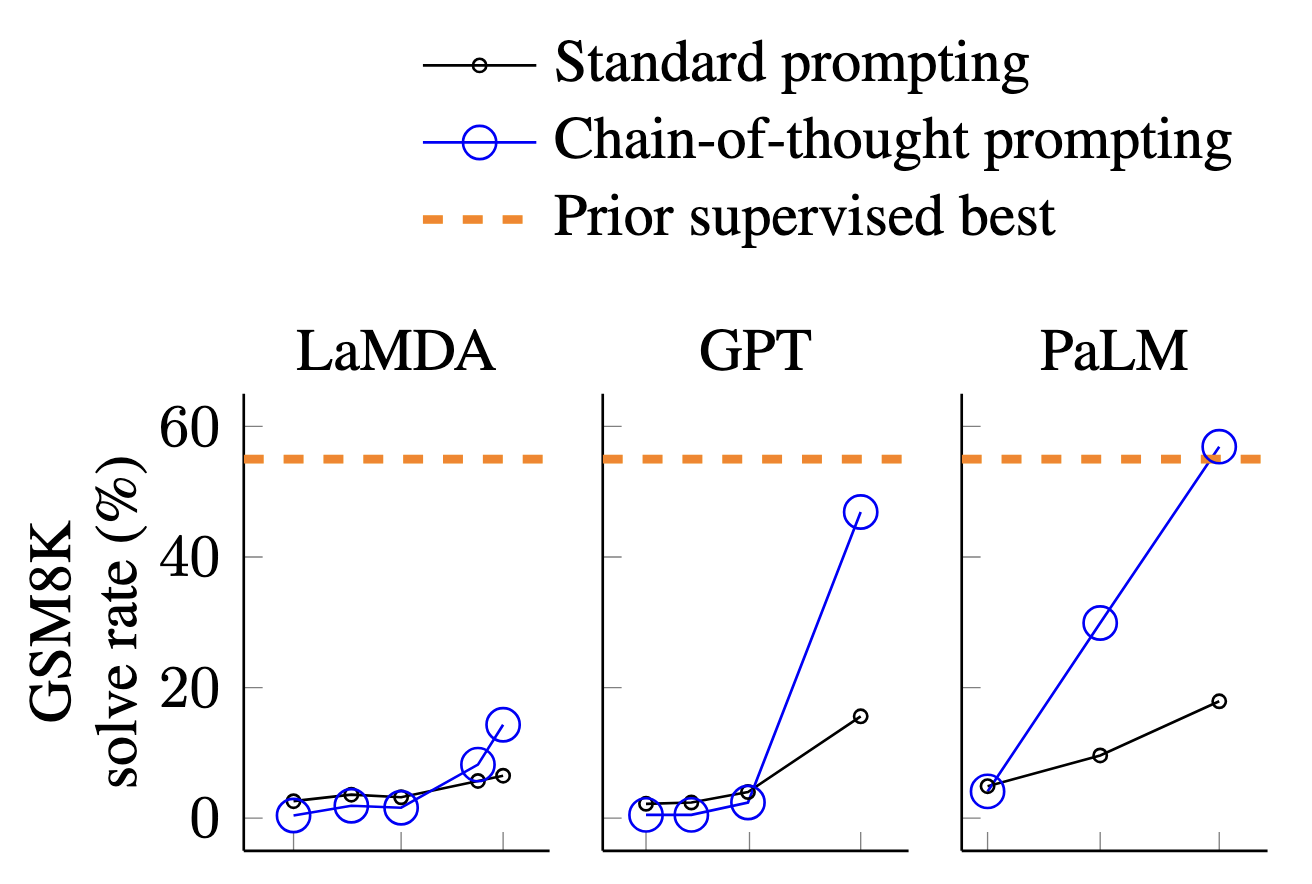
\includegraphics[height = 5.95cm]{figure/cotperformance} 
	\end{figure}

\vfill

\end{frame}

% ------------------------------------------------------------------------------

\begin{frame}{\cotp improves commonsense}

\vfill

\devour{CSQA: Contains around 200K dialogs with a total of 1.6M
turns. Further, unlike existing large scale QA datasets
which contain simple questions that can be answered from a
single tuple, the questions in the dialogs require a larger
subgraph of the KG. }


\begin{figure}
    \centering
    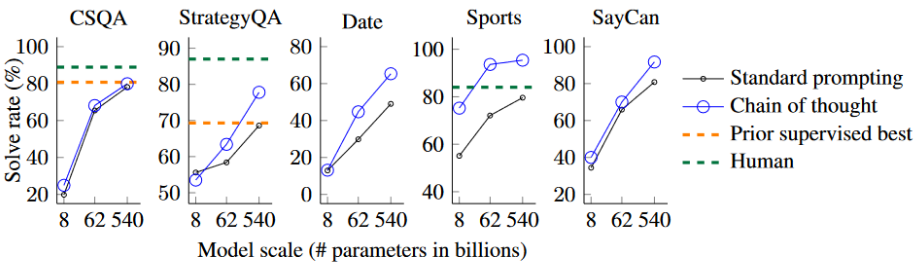
\includegraphics[width=0.9\textwidth]{figure/cot_performance2.png}\\
    \citebutton{Source: Wei et al., 2022}{https://arxiv.org/pdf/2201.11903.pdf}
\end{figure}

\vfill

\end{frame}

%%%%%%%%%%%%%%%%%%%%%%%%%%%%%%%%%%%%%%%%%%%%%%%%%%%%%%%%%%%%%%%%%%%%
\section{Reasoning Models: DeepSeek-R1}
%%%%%%%%%%%%%%%%%%%%%%%%%%%%%%%%%%%%%%%%%%%%%%%%%%%%%%%%%%%%%%%%%%%%
% Source: DL4NLP chapter09-llm/slides-94-deepseek.tex

\begin{frame}{Sources}

\vfill

\begin{itemize}
    \item First major open
    reasoning LM (as opposed to proprietary closed):
    DeepSeek 
\item \citebutton{DeepSeek-AI, 2025}{https://arxiv.org/abs/2501.12948}
\item \citebutton{Nature, 2025}{https://www.nature.com/articles/s41586-025-09422-z}
\end{itemize}

\vfill

\end{frame}

% ------------------------------------------------------------------------------

\begin{vbframe}{Data for SFT: 40B tokens!}

\vfill

\begin{figure}
    \centering
    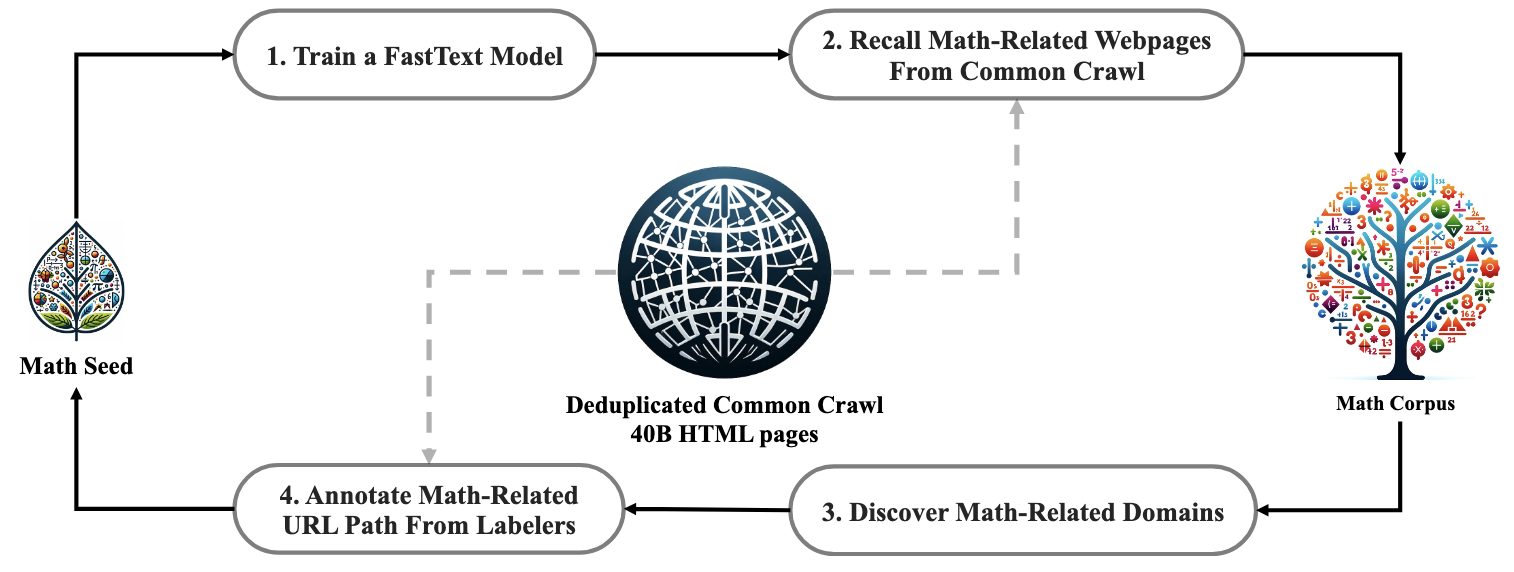
\includegraphics[width=12cm]{figure/deepseekmath.png}
\end{figure}

\citebutton{DeepSeekMath, 2024}{https://arxiv.org/pdf/2402.03300}

\vfill

\end{vbframe}

% ------------------------------------------------------------------------------

\begin{vbframe}{Reinforcement learning}

\vfill

\begin{itemize}
\item In reinforcement learning, an agent takes a sequence
    of actions towards a goal and gets feedback on the
    success of that sequence at the end.
    \item For reasoning trajectories, the feedback is:
    correct or incorrect.
\item (thanks to Emma Brunskill) \begin{tabular}{l@{\hspace{0.2cm}}ll}
& supervised learning & reinforcement learning\\\hline
goal&optimal predictor & optimal policy\\ 
learn from experience? & yes & yes\\
generalization? & yes & yes\\
feedback & rich (each token) & sparse (in/correct)\\
feedback when? & immediately & delayed\\
exploration? & no & yes
\end{tabular}

\end{itemize}

\vfill

\end{vbframe}

% ------------------------------------------------------------------------------

\begin{frame}{Reasoning traces: Format}

\vfill
\begin{itemize}
\item 
The User asks a
question and the Assistant solves it.
\item The Assistant first
thinks about the reasoning process ``in its mind'' and then
provides  the answer to the User.
\item The reasoning process and
answer are enclosed within <think>...</think> and
<answer>...</answer> tags
\item \texttt{<think> reasoning process here </think>}
\item \texttt{<answer> answer here </answer>}
\item ``We intentionally limit our constraints to this
structural format, avoiding any content-specific biases to
ensure that we can accurately observe the natural
progression of the model during the RL process.''
\item So this is not a few-shot approach!
\end{itemize}

\vfill

\end{frame}

% ------------------------------------------------------------------------------

\begin{vbframe}{Example of a reasoning trace}

\vfill

\begin{tabular}{lp{2cm}}
    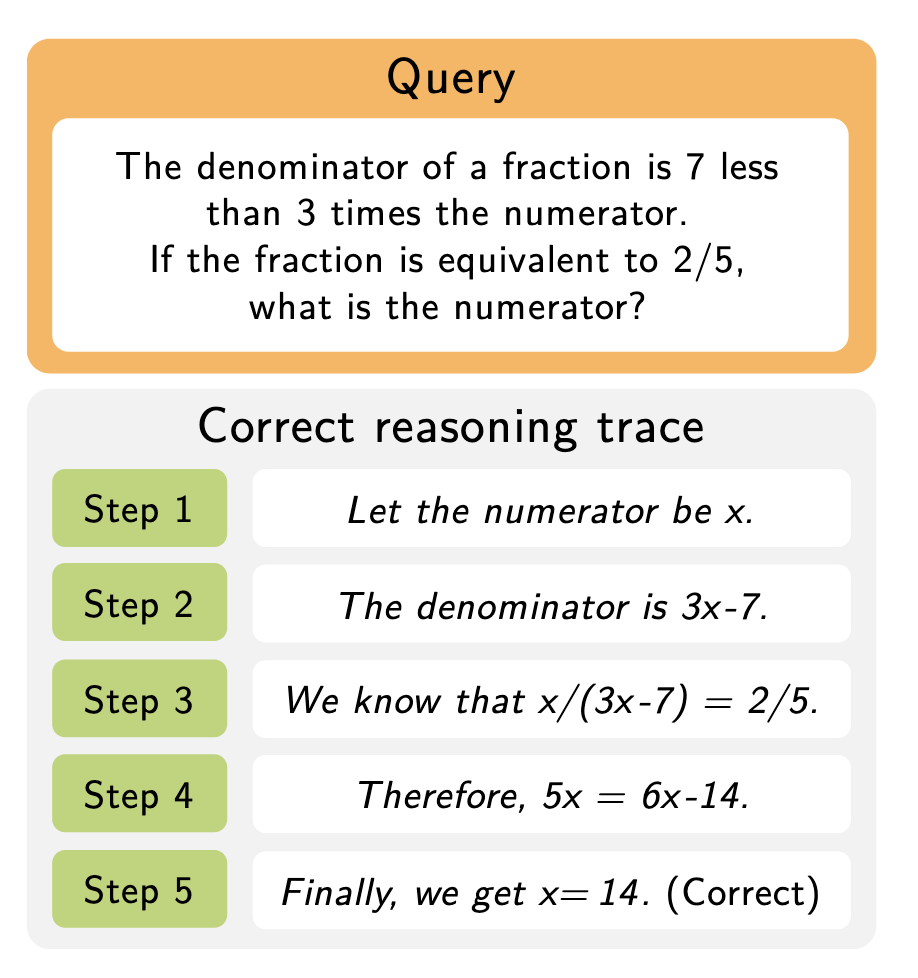
\includegraphics[width=5.78cm]{figure/reasoning,trace}&
\vspace{-5cm} \ques Is this chain of thought few-shot prompting? 
\end{tabular}

\vfill

\end{vbframe}

% ------------------------------------------------------------------------------

\begin{frame}{Automatic, non-human rewards\\ for
    LM-generated reasoning traces}

\vfill

\begin{block}{}
Accuracy rewards evaluate whether the response is
correct. For
example, in the case of maths problems with deterministic
results,
the model is required to provide the final answer in a
specified format
(for example, within a box), enabling reliable rule-based
verification of
correctness. Similarly, for code competition prompts, a
compiler can
be used to evaluate the responses of the model against a
suite of predefined test cases, thereby generating objective feedback on correctness.
\end{block}

\vfill

\end{frame}

% ------------------------------------------------------------------------------

\begin{vbframe}{Automatic verifier/verifiable rewards: AIME example}

\vfill

\begin{figure}
    \centering
    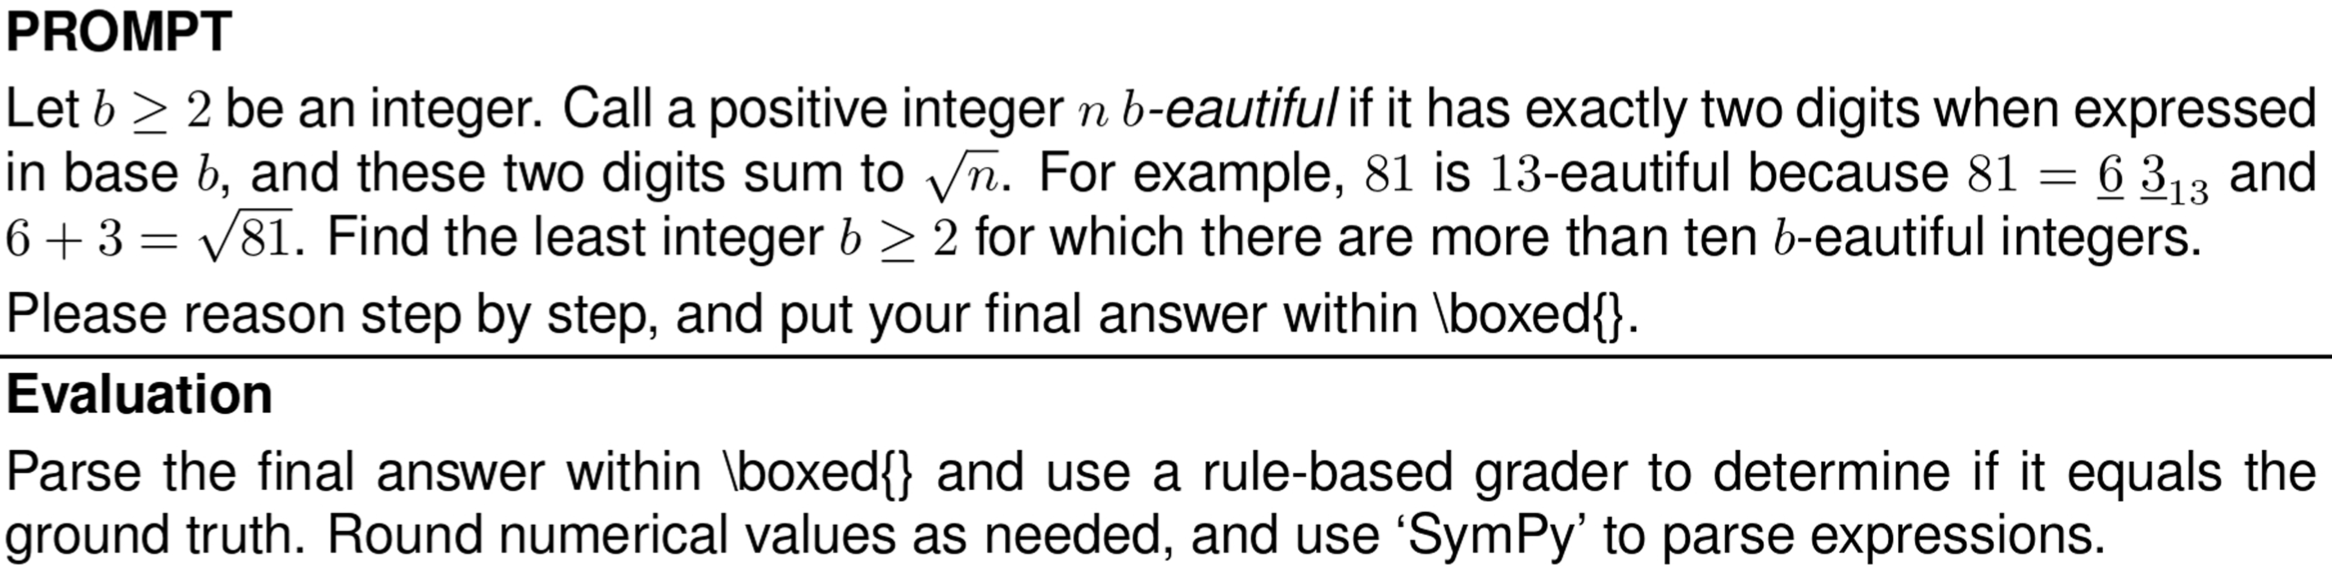
\includegraphics[width=11.5cm]{figure/aime,example}
\end{figure}

\vfill

\end{vbframe}

% ------------------------------------------------------------------------------

\begin{vbframe}{Aha moment}

\vfill

\begin{figure}
    \centering
    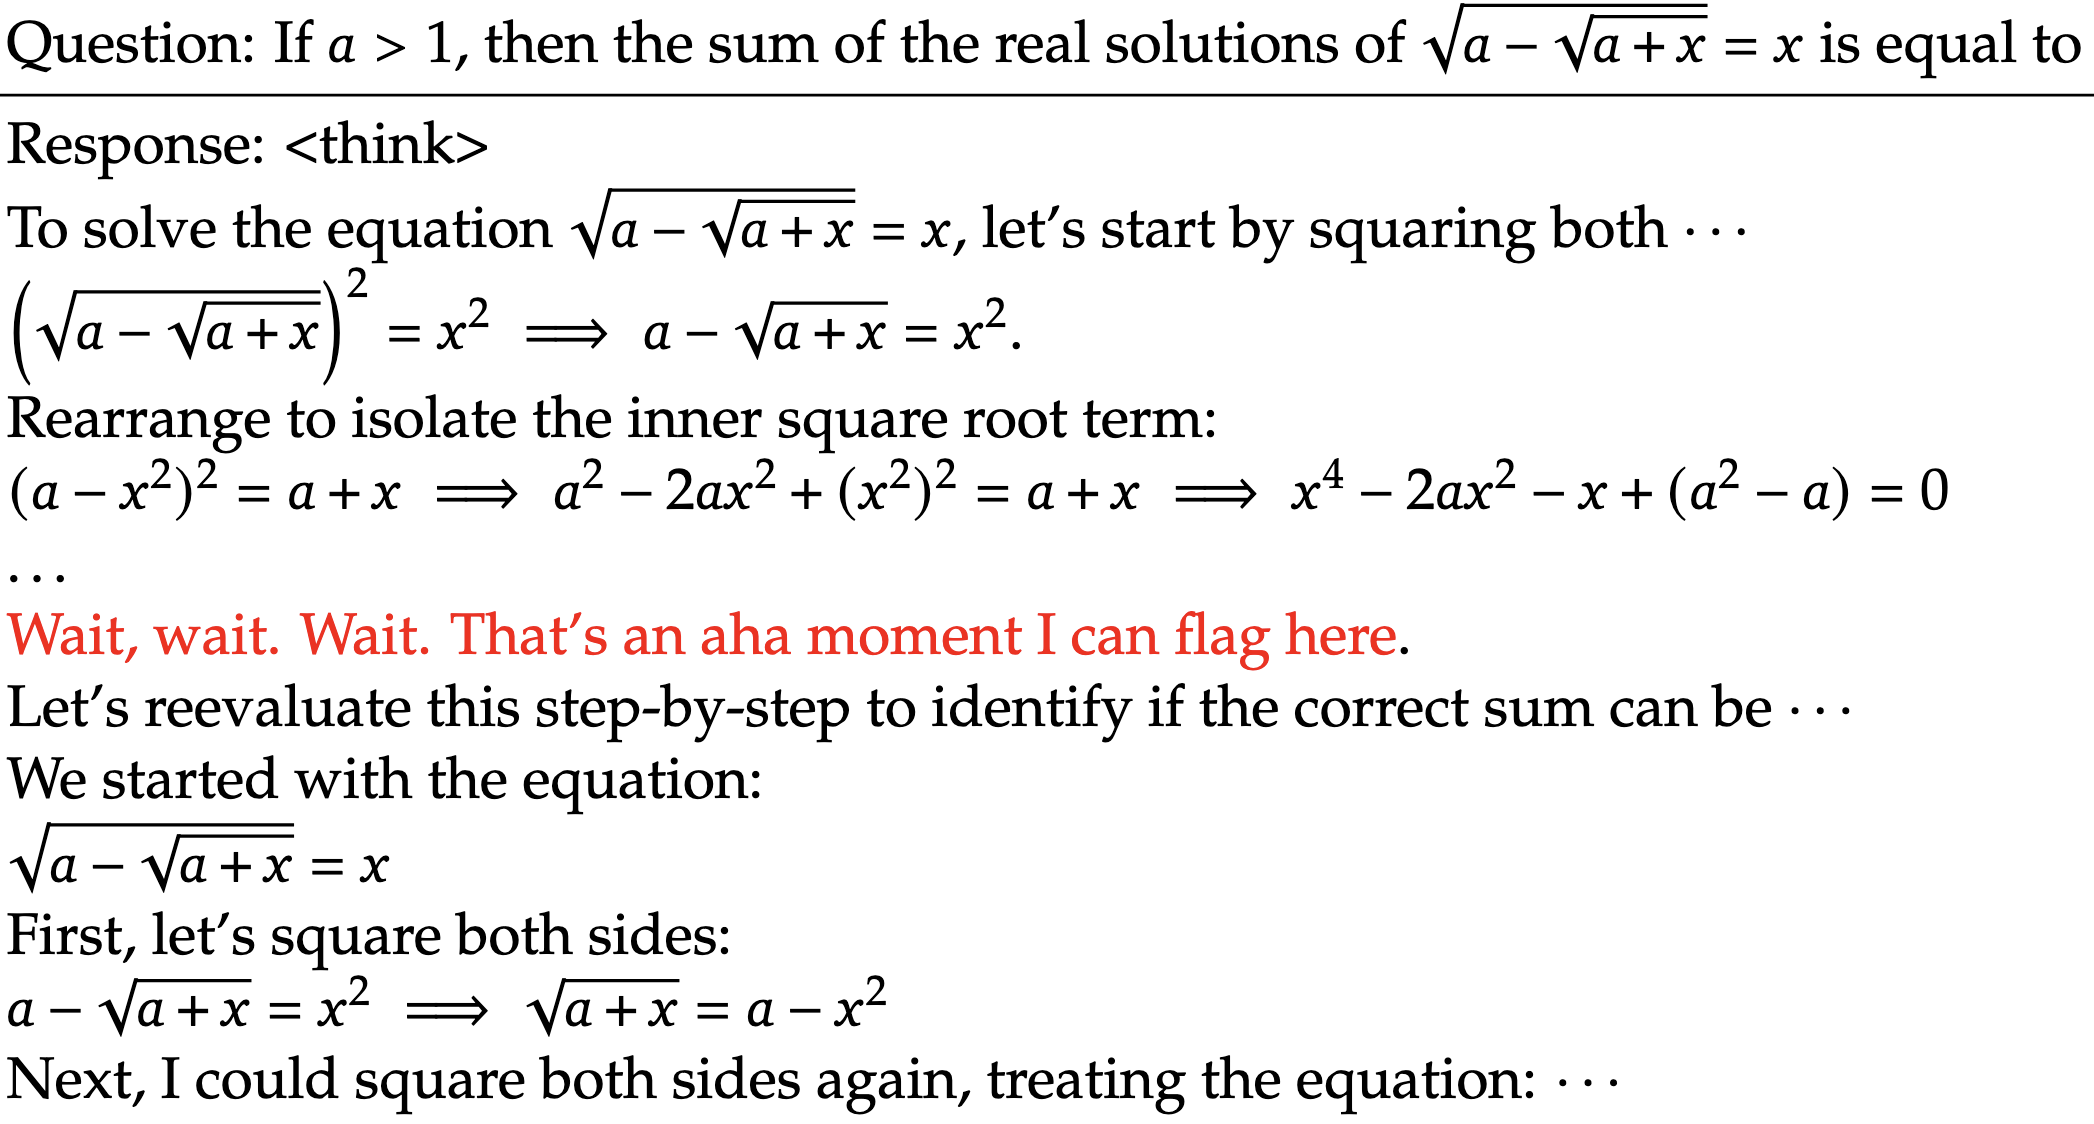
\includegraphics[width=10cm]{figure/ahamoment}
\end{figure}

\vfill

\end{vbframe}

% ------------------------------------------------------------------------------

\begin{frame}{Accuracy AIME: Above human average}
% fit16:9: frame instead of vbframe (vbframe pushed the figure to an otherwise empty second page)

\vfill

\begin{figure}
    \centering
    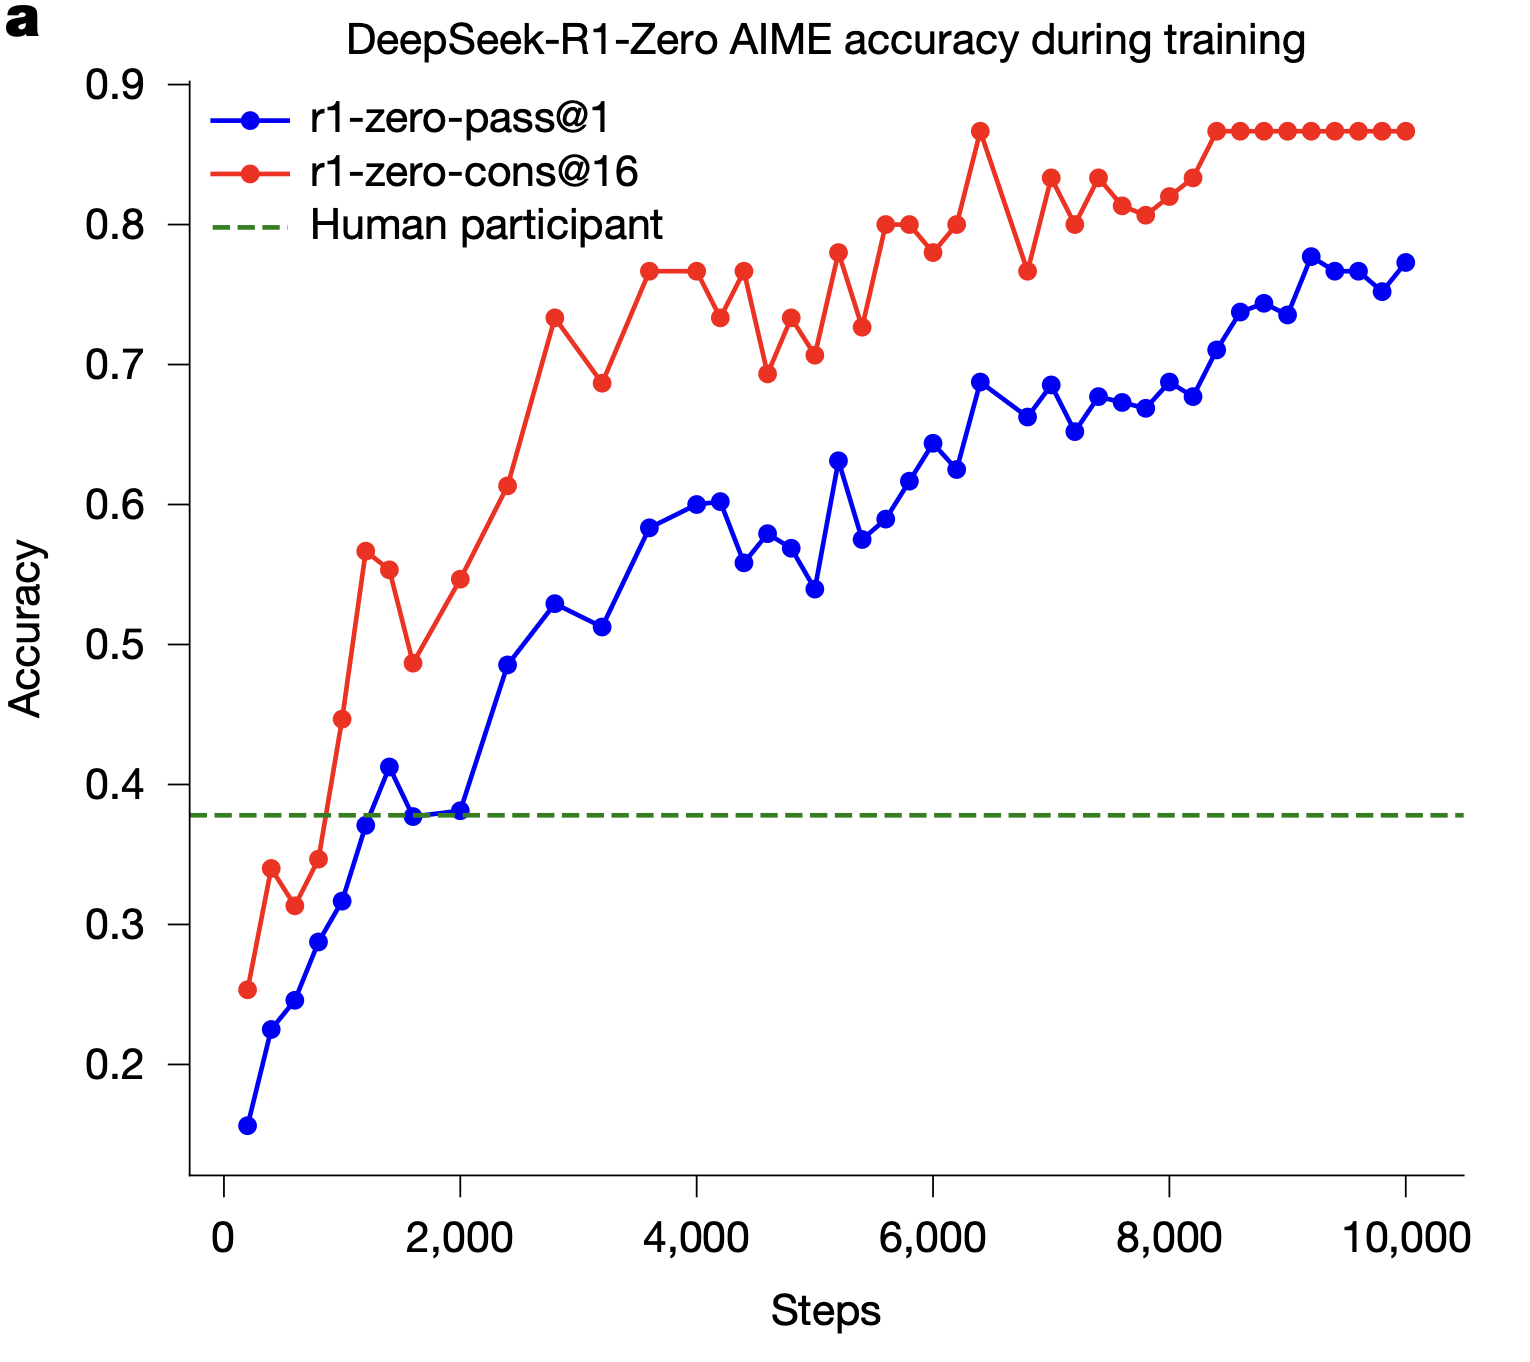
\includegraphics[width=6.80cm]{figure/accuracy,aime.png}
\end{figure}

\vfill

\end{frame}

% ------------------------------------------------------------------------------

\begin{vbframe}{Unfaithfulness of LMs to true reasoning}

\vfill

\begin{figure}
    \centering
    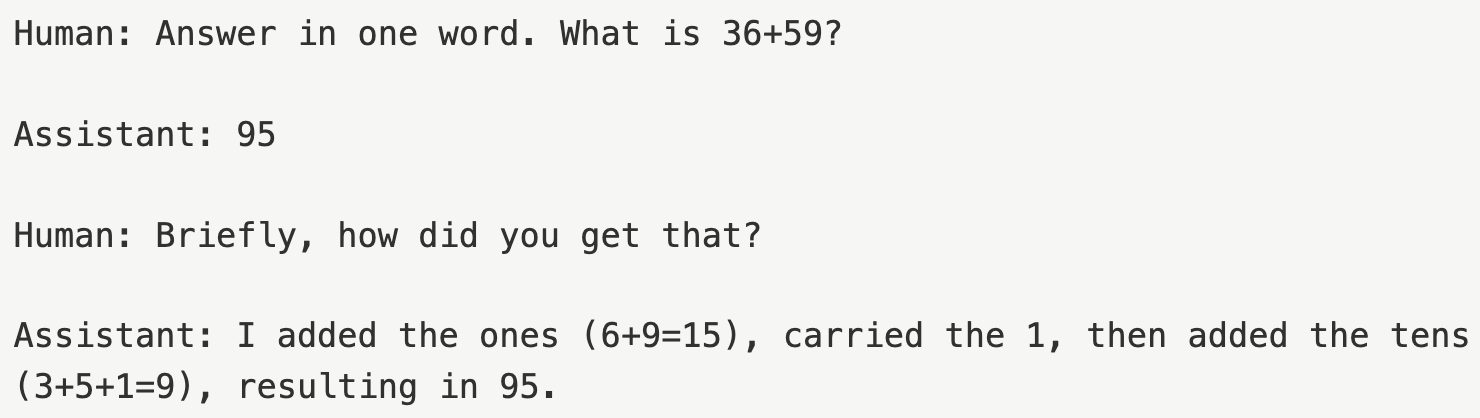
\includegraphics[width=12cm]{figure/sixplusnine,0.png}
\end{figure}

\vfill

\end{vbframe}

% ------------------------------------------------------------------------------

\begin{vbframe}{Unfaithfulness of LMs to true reasoning}

\vfill

\begin{figure}
    \centering
    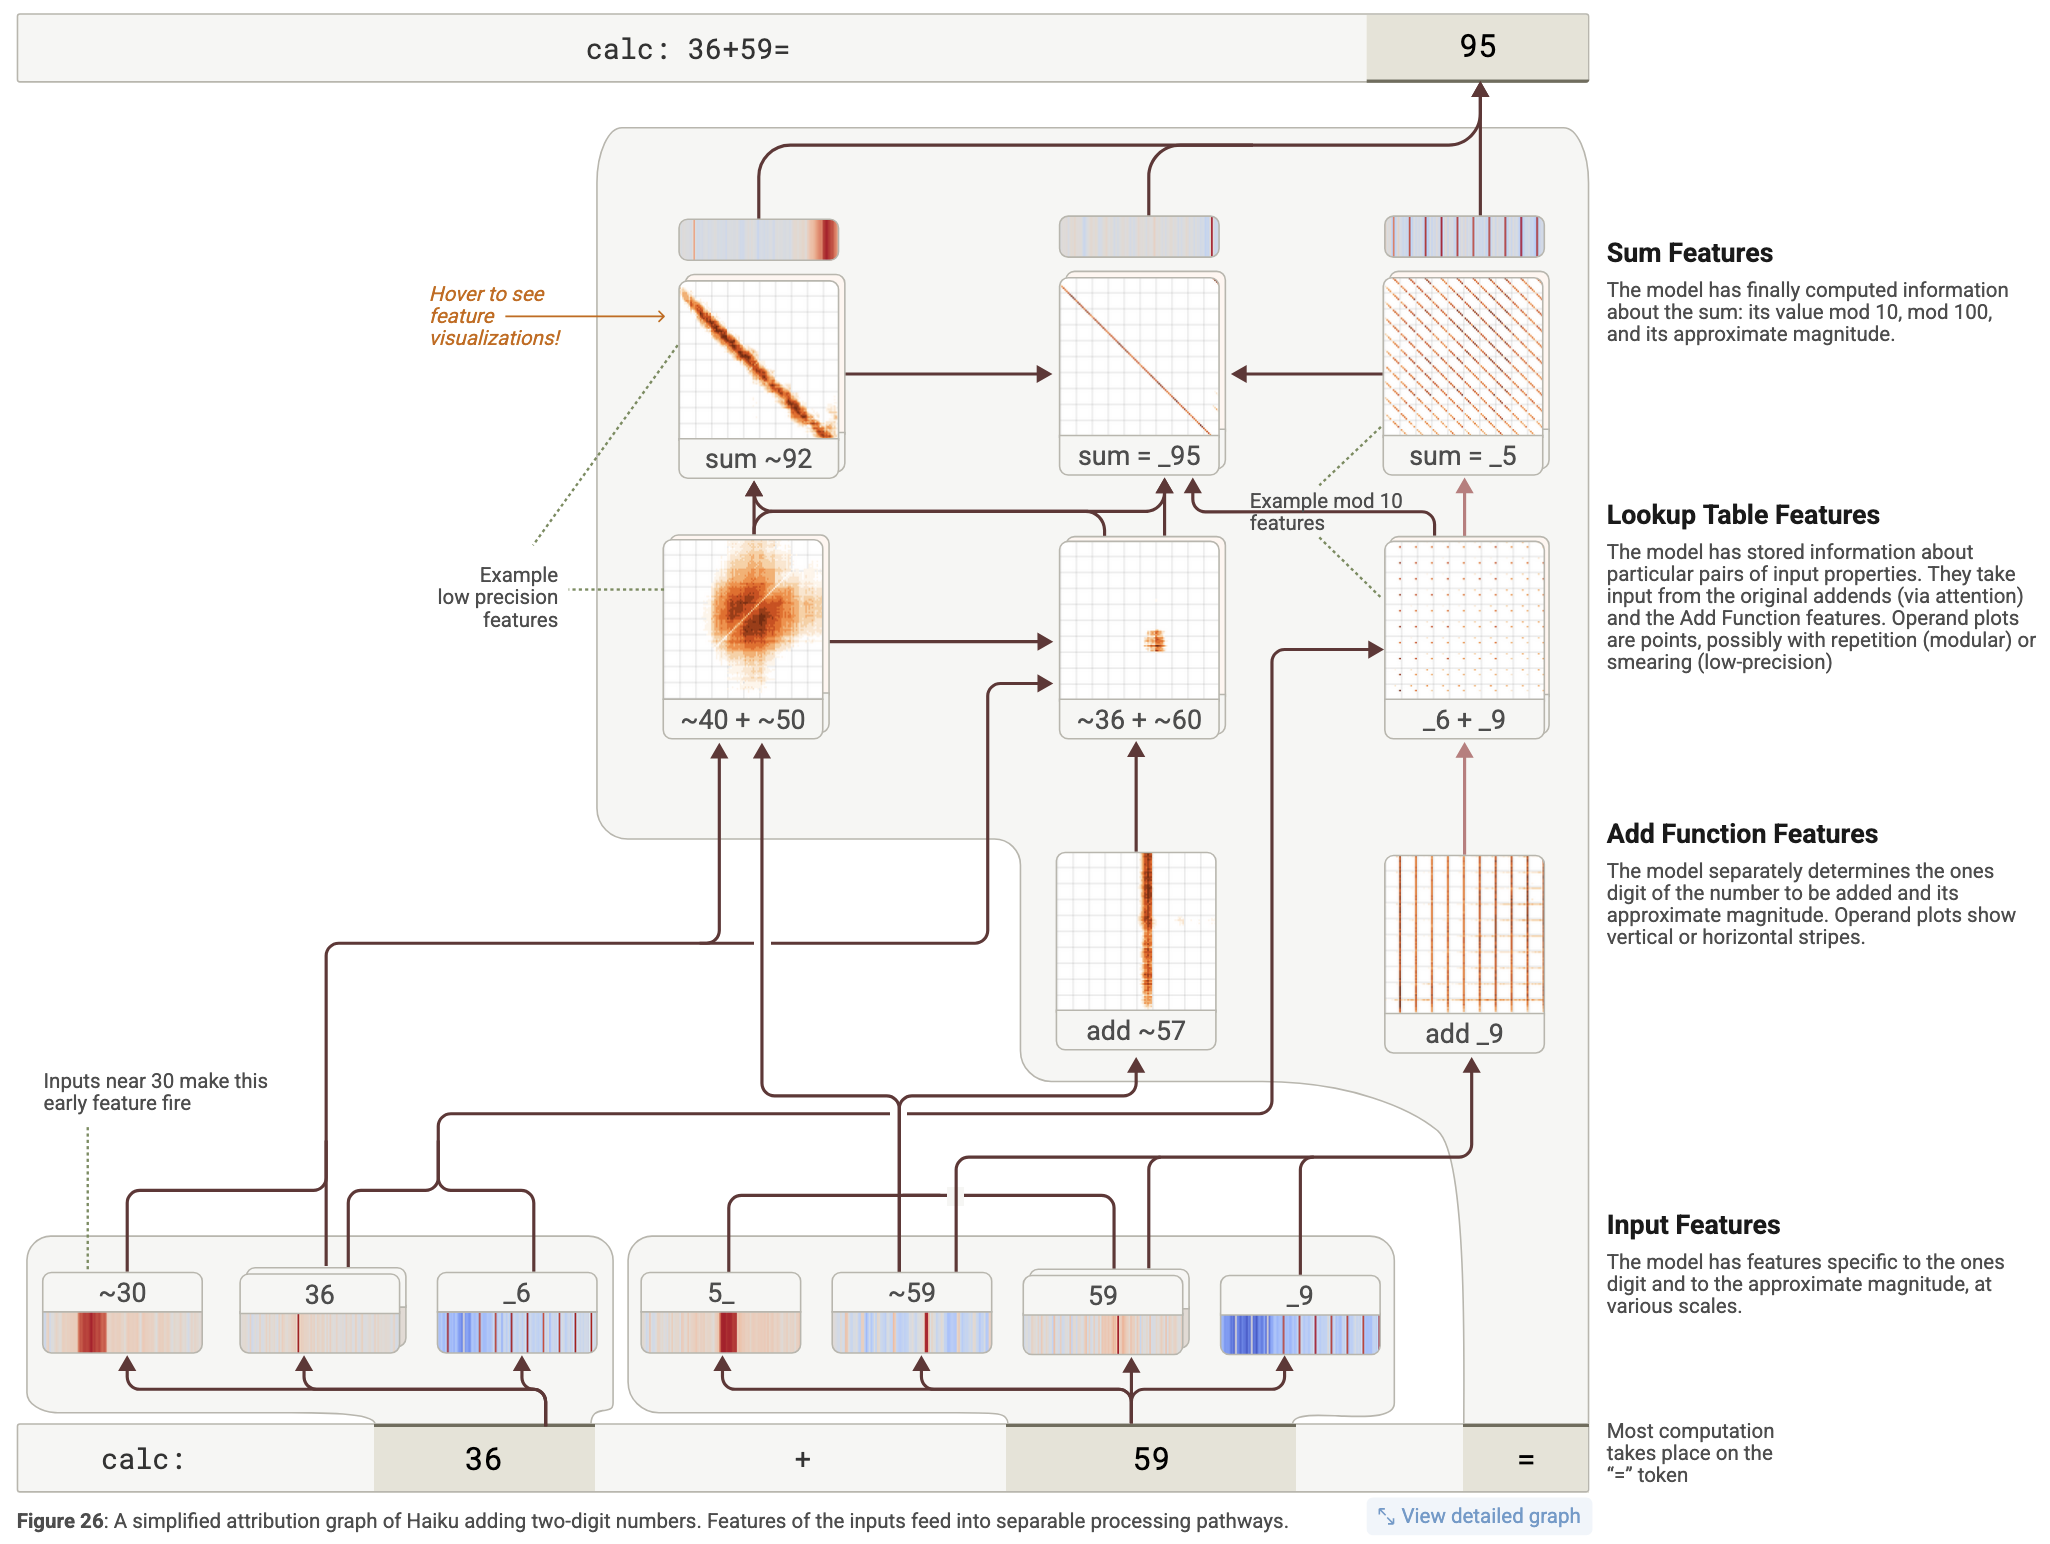
\includegraphics[width=7.65cm]{figure/sixplusnine,1.png}
\end{figure}

\vfill

\end{vbframe}

%%%%%%%%%%%%%%%%%%%%%%%%%%%%%%%%%%%%%%%%%%%%%%%%%%%%%%%%%%%%%%%%%%%%
\section{Where This Is Going}
%%%%%%%%%%%%%%%%%%%%%%%%%%%%%%%%%%%%%%%%%%%%%%%%%%%%%%%%%%%%%%%%%%%%
% [O] original bridge text (draft for the user to review); listed in order.txt
\begin{vbframe}{Where This Is Going}
\begin{itemize}
  \item Session 9 looks inside the Transformer block: what has changed since 2017 (normalization, activations, position embeddings, attention variants) and mixture-of-experts models such as DeepSeek-V3.
  \item Session 10 shows that nothing in this session is specific to text: the same encoder-only, decoder-only, and encoder-decoder patterns, and the same pretrain-then-adapt recipe, drive vision and multimodal models.
  \item DeepSeek-R1's training loop (rewards from automatic verifiers instead of labels) is reinforcement learning --- the subject of session 11.
\end{itemize}
\end{vbframe}


%%%%%%%%%%%%%%%%%%%%%%%%%%%%%%%%%%%%%%%%%%%%%%%%%%%%%%%%%%%%%%%%%%

\section{License \& Attribution}
%%%%%%%%%%%%%%%%%%%%%%%%%%%%%%%%%%%%%%%%%%%%%%%%%%%%%%%%%%%%%%%%%%

\begin{frame}{License \& Attribution}
\footnotesize
\begin{itemize}
\item \textbf{Main source.} All sections except those listed below are adapted from \textbf{Deep Learning for NLP (DL4NLP)}, SLDS, LMU Munich, chapters 4 (\textit{BERT}), 6 (\textit{Post-BERT Era}), 7 (\textit{Generative Pre-Trained Transformers}), 8 (\textit{Decoding Strategies}) and 9 (\textit{Large Language Models}) --- licensed \textbf{CC BY 4.0}: \url{https://creativecommons.org/licenses/by/4.0/}. Frames were reordered (GPT first) and selected; the few edits inside frames are listed in \texttt{order.txt}. The \enquote{Excursus: ELMo} frame takes its bullets from DL4NLP chapter 2 (\textit{Deep Learning Basics}, file \enquote{ELMo}).
\item Figures are reproduced as they appear in DL4NLP, with the attributions DL4NLP itself gives.
\item \textbf{Original to this course.} \enquote{Recap: Three Transformer Families}, \enquote{Today: Pretrain, Then Adapt}, \enquote{From GPT to BERT} and \enquote{Where This Is Going}.
\item The two earlier, longer decks this session was merged from (BERT \& T5; LLMs) remain in \texttt{\_previous/}.
\end{itemize}
\end{frame}

\endlecture
\end{document}
